\documentclass[11pt,letterpaper,titlepage]{article}

%================== Document nomenclature
\newcommand{\DOCSUBJT}{Whitepaper: }   %Put document subject here
\newcommand{\DOCTITLE}{                      %Put document title here
	The Linear Boltzman Solver - a Discrete Ordinates Method solver 
}       
\newcommand{\DOCDATE} {September, 2019}         %Put document date here
\newcommand{\DOCREV}  {Rev 1.00}             %Put revision number here

%================== Misc Settings
\usepackage{fancyhdr}
\usepackage[left=0.75in, right=0.75in, bottom=1.0in]{geometry}
\usepackage{lastpage}
\usepackage{titleref}
\usepackage{booktabs}
\usepackage{appendix}

\appendixtitleon
\appendixtitletocon

\makeatletter

%================== List of figures and tables mods
\usepackage{tocloft}
\usepackage[labelfont=bf]{caption}

\renewcommand{\cftfigpresnum}{Figure\ }
\renewcommand{\cfttabpresnum}{Table\ }

\newlength{\mylenf}
\settowidth{\mylenf}{\cftfigpresnum}
\setlength{\cftfignumwidth}{\dimexpr\mylenf+3.5em}
\setlength{\cfttabnumwidth}{\dimexpr\mylenf+1.5em}



%=================== Misc packages
\usepackage{graphicx}
\usepackage[breakwords]{truncate}
\usepackage{float}
\usepackage{array}
\usepackage{amsmath}
\usepackage{mdframed}
\usepackage{fancyvrb}
\usepackage{float}
\usepackage{cancel}
\usepackage{amssymb}
\graphicspath{ {images/} }
\usepackage[usenames,dvipsnames,svgnames,table]{xcolor}
%\usepackage[defaultlines=2,all]{nowidow}
\usepackage{listings}
\usepackage{color}
\definecolor{Brown}{cmyk}{0,0.81,1,0.60}
\definecolor{OliveGreen}{cmyk}{0.64,0,0.95,0.40}
\definecolor{CadetBlue}{cmyk}{0.62,0.57,0.23,0}
\usepackage{pdflscape}
\usepackage{relsize}
\usepackage{verbatim}
\usepackage{tabto}
%\usepackage{upgreek}
\usepackage{enumitem}
%\usepackage{MnSymbol}% http://ctan.org/pkg/mnsymbol
\usepackage[pdf]{graphviz}
\usepackage[linesnumbered,lined,boxruled,algosection,commentsnumbered]{algorithm2e}
\usepackage{enumitem}
%\usepackage[displaymath, mathlines,running]{lineno}

\definecolor{gray}{rgb}{0.4,0.4,0.4}
\definecolor{darkblue}{rgb}{0.0,0.0,0.6}
\definecolor{cyan}{rgb}{0.0,0.6,0.6}

\definecolor{ao(english)}{rgb}{0.0, 0.5, 0.0}

\newcommand{\xmltag}[1]{\textcolor{blue}{ \texttt{#1}} }
\newcommand{\xmloption}[1]{\textcolor{ao(english)}{ \texttt{#1}} }


\counterwithin{figure}{section}
\renewcommand{\thefigure}{\arabic{section}.\arabic{figure}}
%=================== Big cdot
\newcommand*\bigcdot{\mathpalette\bigcdot@{.5}}
\newcommand*\bigcdot@[2]{\mathbin{\vcenter{\hbox{\scalebox{#2}{$\m@th#1\bullet$}}}}}

\newcommand{\beq}{\begin{equation*}
\begin{aligned}}
\newcommand{\eeq}{\end{aligned}
\end{equation*}}

\newcommand{\beqn}{\begin{equation}
	\begin{aligned}}
\newcommand{\eeqn}{\end{aligned}
	\end{equation}}

%=================== Settings
\renewcommand{\baselinestretch}{1.2}
\definecolor{gray}{rgb}{0.4 0.4 0.4}
\newcommand{\stimes}{{\times}}

%================== Code syntax highlighting
\lstset{language=C++,frame=ltrb,framesep=2pt,basicstyle=\linespread{0.8} \small,
	keywordstyle=\ttfamily\color{OliveGreen},
	identifierstyle=\ttfamily\color{CadetBlue}\bfseries,
	commentstyle=\color{Brown},
	stringstyle=\ttfamily,
	showstringspaces=true,
	tabsize=2,}
	
%================== Section numbers with equation numbers
\numberwithin{equation}{section}


%================== Short \to arrow
\setlength{\medmuskip}{0mu}
%\newcommand{\tos}[1][3pt]{\mathrel{%
%   \hbox{\rule[\dimexpr\fontdimen22\textfont2-.2pt\relax]{#1}{.4pt}}%
%   \mkern-4mu\hbox{\usefont{U}{lasy}{m}{n}\symbol{41}}}}



\setlength\parindent{0pt}


\begin{document}

\begin{titlepage}
\pagestyle{fancy}
\vspace*{1.0cm}
\centering
\vspace{1cm}
\vspace{.25cm}
{\Large\bfseries  \DOCSUBJT \par} 
{\Large\bfseries \DOCTITLE  \par}
\vspace{1cm}
{\Large \DOCDATE \par}
\vspace{1.0cm}
{\Large Jan Vermaak \par}
{\Large \DOCREV \par}

\begin{center}
	\begin{minipage}[c]{0.45\textwidth}
		\begin{figure}[H]
			
			
\includegraphics[width=3in]{Figures/Logo2_Medium.png}
		\end{figure}
	\end{minipage}
\end{center}

\end{titlepage}	


\pagestyle{fancy}
\rfoot{Page \thepage \ of \pageref{LastPage}}
\cfoot{}
\lfoot{\truncate{14cm}{\DOCTITLE}}
\rhead{}
\chead{\currentname}
\lhead{}
\renewcommand{\footrulewidth}{0.4pt}

\newpage
\chead{Table of contents}
%\begin{comment}
\tableofcontents
\addtocontents{toc}{~\hfill\textbf{Page}\par}

\listoffigures
\listoftables

%\end{comment}
\chead{Contents}	

%#########################################################################
%\linenumbers
\newpage
\chead{Basics - The Linear Boltzman Transport Equation}
\section{Basics - The Linear Boltzman Transport Equation}
Let us denote the position of a particle in space by $\mathbf{r}=[x \ y \ z]$ and the direction along which it is traveling by the normal vector $\hat{\Omega}$ such that

$$\hat{\Omega} = [\sin \theta . \cos \varphi \quad \sin \theta . \sin \varphi \quad \cos \theta]$$

\begin{figure}[h]
\centering
\includegraphics[width=0.5\linewidth]{Figures/PositionOmega}
\caption{Orientation of direction in cartesian space.}
\label{fig:positionomega}
\end{figure}

Now we want to observe a control volume and the balance of particles within it. But first we have to define a few terms. First is the particle density $n$, with units $[\frac{particles}{cm^3}]$, dependent on position, direction and energy, written as
$$n(r,\hat{\Omega},E,t).$$
\noindent For this scope we will drop the notion of time dependence. Particle density can be multiplied by the velocity associated with its energy to determine the angular flux $\Psi$, written as
$$
\Psi (r,E,\hat{\Omega}) = v(E) n(r,E,\hat{\Omega}).
$$
\noindent This has units of $[\frac{particles}{cm^2 s}]$ and is essential to couple reactions to known cross-sections in the form of
$$\text{Reaction rate}=\Sigma_t \Psi$$

\noindent Let us now turn our attention to the balance of particles in a control volume.
\newpage


\begin{figure}[h]
    \centering
    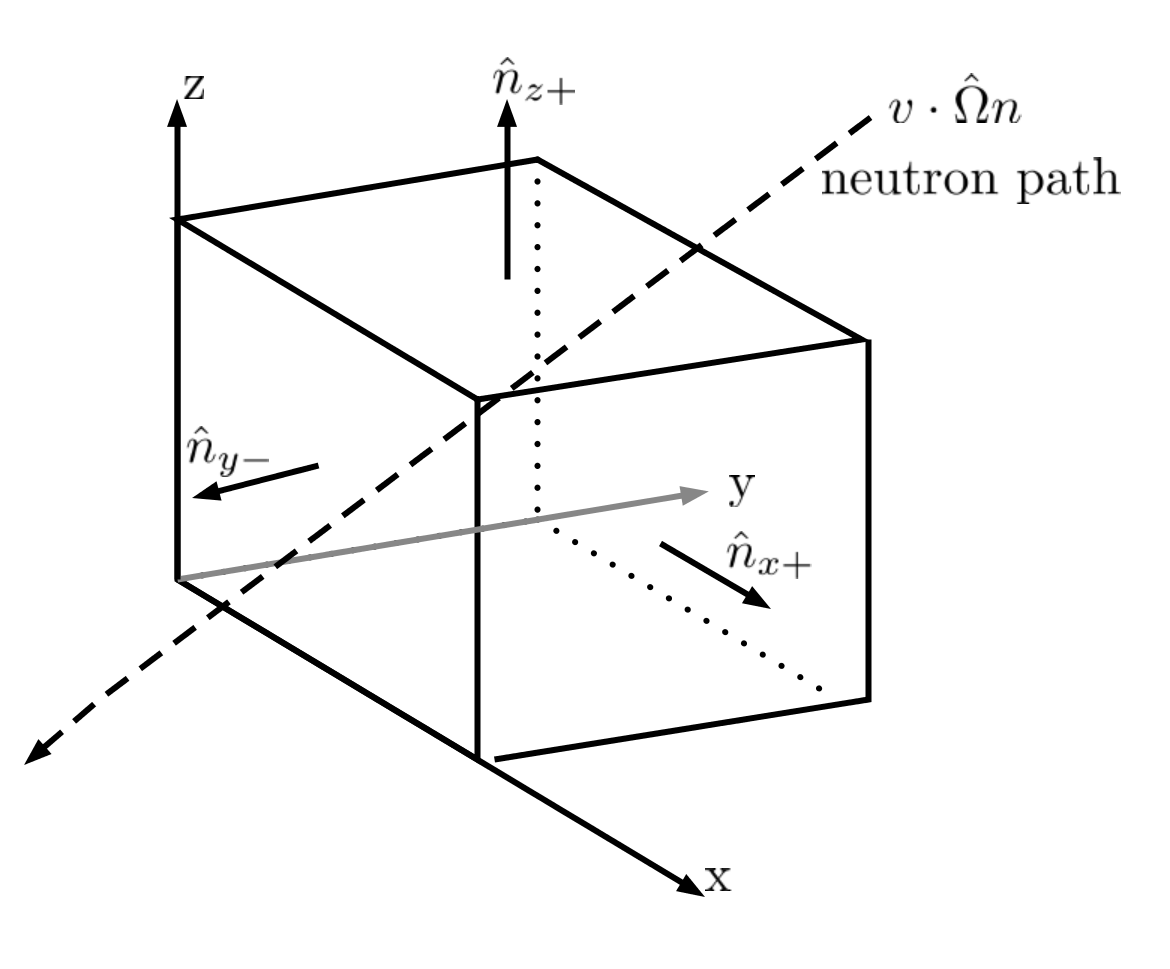
\includegraphics[width=0.4\linewidth]{Figures/ControlVolume}
    \caption{Control volume for neutron balance.}
    \label{fig:controlvolume}
\end{figure}
\noindent
Consider the control volume as shown in figure \ref{fig:controlvolume}. The time rate of change of neutrons over the volume $\frac{dn}{dt}$ is given by

\begin{equation}
\begin{aligned}
\int_{dV}\frac{dn}{dt}.dr = 0
&= -\int_{S} \biggr[ \hat{n} \bigcdot \hat{\Omega} \Psi (r,E,\hat{\Omega})   \biggr]. dA
 -\int_{dV} \Sigma_a (r,E)\Psi(r,E,\hat{\Omega}).dr\\
&-\int_{dV}  \int_E \int_{4\pi} 
\Sigma_s (r,E{\to}E',\hat{\Omega} {\to} \hat{\Omega}') \Psi (r,E,\hat{\Omega}) 
.d\hat{\Omega}'.dE'.dr\\
&+\int_{dV}  \int_E \int_{4\pi}
\Sigma_s (r,E'{\to} E,\hat{\Omega}' {\to} \hat{\Omega}) \Psi (r,E',\hat{\Omega}') 
.d\hat{\Omega}'.dE'.dr\\
&+\frac{\chi (E)}{4\pi} 
\int_{dV}  \int_E \int_{4\pi} 
\Sigma_f (r,E',\hat{\Omega}') \Psi (r,E',\hat{\Omega}') 
.d\hat{\Omega}'.dE'.dr\\
&+\int_{dV} Q_{fixed}(r,E,\hat{\Omega}).dr
\end{aligned}
\end{equation}
\newline
Gauss's divergence theorem on the streaming term:

\begin{equation*}
\int_{S} \biggr[ \hat{n} \bigcdot  \hat{\Omega}\Psi (r,E,\hat{\Omega})   \biggr]. dA = 
\int_{dV} \biggr[ \hat{\Omega}\nabla \Psi (r,E,\hat{\Omega})   \biggr]. dr
\end{equation*}
\newline
Now:
\begin{equation}
\begin{aligned}
\int_{dV}\frac{dN}{dt}.dr = 0
&= -\int_{dV} \biggr[ \hat{\Omega}\nabla \Psi (r,E,\hat{\Omega})   \biggr]. dr
-\int_{dV} \Sigma_a (r,E)\Psi(r,E,\hat{\Omega}).dr\\
&-\int_{dV}  \int_E \int_{4\pi} 
\Sigma_s (r,E{\to} E',\hat{\Omega} {\to} \hat{\Omega}') \Psi (r,E,\hat{\Omega}) 
.d\hat{\Omega}'.dE'.dr\\
&+\int_{dV}  \int_E \int_{4\pi}
\Sigma_s (r,E'{\to} E,\hat{\Omega}' {\to} \hat{\Omega}) \Psi (r,E',\hat{\Omega}') 
.d\hat{\Omega}'.dE'.dr\\
&+\frac{\chi (E)}{4\pi} 
\int_{dV}  \int_E \int_{4\pi} 
\Sigma_f (r,E',\hat{\Omega}') \Psi (r,E',\hat{\Omega}') 
.d\hat{\Omega}'.dE'.dr\\
&+\int_{dV} Q_{fixed}(r,E,\hat{\Omega}).dr
\end{aligned}
\end{equation}

\noindent Dropping all the $\int_{dV}.dr$ gives:
\begin{equation}
\begin{aligned}
 0
&= -\hat{\Omega} \nabla \Psi (r,E,\hat{\Omega})
- \Sigma_a (r,E)\Psi(r,E,\hat{\Omega})\\
&-  \int_E \int_{4\pi} 
\Sigma_s (r,E{\to} E',\hat{\Omega} {\to} \hat{\Omega}') \Psi (r,E,\hat{\Omega}) 
.d\hat{\Omega}'.dE'\\
&+  \int_E \int_{4\pi}
\Sigma_s (r,E'{\to} E,\hat{\Omega}' {\to} \hat{\Omega}) \Psi (r,E',\hat{\Omega}') 
.d\hat{\Omega}'.dE'\\
&+\frac{\chi (E)}{4\pi} 
  \int_E \int_{4\pi} 
\Sigma_f (r,E',\hat{\Omega}') \Psi (r,E',\hat{\Omega}') 
.d\hat{\Omega}'.dE'\\
&+ Q_{fixed}(r,E,\hat{\Omega})
\end{aligned}
\end{equation}
\newline
If we leave the NTE in this form we will do the scattering integral over all energy groups where neutrons are scattering to this group, and another integral over all energy groups where neutrons are scattering from this group to another. To reduce the complexity/difficulty of this we combine the scattering from group $E$ to $E'$ into the total removal cross-section:

\begin{equation*}
\begin{aligned}
\Sigma_t (r,E,\hat{\Omega})\Psi(r,E,\hat{\Omega}) &=  \Sigma_a (r,E)\Psi(r,E,\hat{\Omega})\\
&+  \int_E \int_{4\pi} 
\Sigma_s (r,E{\to} E',\hat{\Omega} {\to} \hat{\Omega}') \Psi (r,E,\hat{\Omega}) 
.d\hat{\Omega}'.dE'\\
\end{aligned}
\end{equation*}
\newline
Which gives us the base NTE:

\begin{equation}
\begin{aligned}
\hat{\Omega}\nabla \Psi (r,E,\hat{\Omega}) 
+\Sigma_t (r,E)\Psi(r,E,\hat{\Omega})
&=  \int_E \int_{4\pi}
\Sigma_s (r,E'{\to} E,\hat{\Omega}' {\to} \hat{\Omega}) \Psi (r,E',\hat{\Omega}') 
.d\hat{\Omega}'.dE'\\
&+\frac{\chi (E)}{4\pi} 
  \int_E \int_{4\pi} 
\Sigma_f (r,E',\hat{\Omega}') \Psi (r,E',\hat{\Omega}') 
.d\hat{\Omega}'.dE'\\
&+ Q_{fixed}(r,E,\hat{\Omega})
\end{aligned}
\end{equation}
\newline
\newline
If we want to remove more complexity we can combine the fission source term into the source to get the Neutron Transport Equation in its most basic form:

\begin{equation} \label{eq:baseNTE}
\begin{aligned}
\biggr(\hat{\Omega}\nabla +\Sigma_t (r,E)\biggr) \Psi(r,E,\hat{\Omega})
&=  \int_E \int_{4\pi}
\Sigma_s (r,E'{\to} E,\hat{\Omega}' {\to} \hat{\Omega}) \Psi (r,E',\hat{\Omega}') 
.d\hat{\Omega}'.dE'\\
&+ Q_{fixed}(r,E,\hat{\Omega})
\end{aligned}
\end{equation}

\newpage
\chead{Expansion of angular functions}
\section{Expansion of angular functions}
\subsection{The scattering Kernel and Legendre expansion}
The scattering cross-section of materials are normally available as a function of energy only. It is up to the user of the data to add the appropriate scattering kernels for which the scattering angles are a function of the masses of the neutron and its colliding nucleus as well as the energy. But first let us express the scattering terms in a Kernel fashion. We start with the scattering source term as is appears in equation \ref{eq:baseNTE}:

\begin{align*}
\int_E \int_{4\pi}
\Sigma_s (r,E'{\to} E,\hat{\Omega}' {\to} \hat{\Omega}) \Psi (r,E',\hat{\Omega}') 
.d\hat{\Omega}'.dE'.\\
\end{align*}

We then split the macroscopic scattering cross-section into an energy dependent but not angularly dependent term, $\Sigma_s (r,E')$, and a separate kernel $K(E'{\to}E,\hat{\Omega}'{\to}\hat{\Omega})$ as 

\begin{align*}
\int_E \int_{4\pi}
\Sigma_s (r,E').K(E'{\to}E,\hat{\Omega}'{\to}\hat{\Omega}).\Psi (r,E',\hat{\Omega}') 
.d\hat{\Omega}'.dE'.\\
\end{align*}
\newline
Naturally, we require 
\begin{align} \label{eq:kernelIntegralUnity}
\int_E\int_{4\pi}
K(E'{\to}E,\hat{\Omega}'{\to}\hat{\Omega}) 
.d\hat{\Omega}.dE=1.
\end{align}
\newline
Now we expand this Kernel using Legendre polynomials but before we do this we have to handle the notion of $\hat{\Omega}'{\to}\hat{\Omega}$. We redefine the kernel as being dependent on the scattering angle $\theta_s$ where

\begin{align*}
cos\theta_s = \hat{\Omega}'\bullet\hat{\Omega} = \mu
\end{align*}

\begin{align*}
K(cos\theta_s,E'{\to}E) &= \sum_{\ell=0}^\infty \frac{2\ell+1}{2} P_\ell (cos\theta_s) K_\ell (E'{\to}E) \text{ or } \\
K(\mu,E'{\to}E) &= \sum_{\ell=0}^\infty \frac{2\ell+1}{2} P_\ell (\mu) K_\ell (E'{\to}E)
\end{align*}

\noindent This expansion is over the entire radial cone $2\pi$ and therefore we include a normalization factor of $\frac{1}{2\pi}$. The scattering term therefore becomes

\begin{align} \label{eq:scatterKernelLegendre}
\Sigma_s (r,E')K(E'{\to}E,\hat{\Omega}'{\to}\hat{\Omega}) = \Sigma_s (r,E')
\sum_{\ell=0}^\infty \frac{2\ell+1}{4\pi} P_\ell (cos\theta_s) K_\ell (E'{\to}E).
\end{align} 

\subsection{Spherical harmonics and Associated Legendre Polynomials}
The entry point for a person researching spherical harmonics is inevitably the wikipedia and wolfram-alpha websites describing the complex valued spherical harmonics. However, from various sources it is evident that we can compute the same expansion by using the real forms of the sperical harmonics, called the \textbf{tesseral spherical harmonics}. This expansion is done in the form

\beqn 
f(\varphi,\theta) = \sum_{\ell = 0}^\infty \sum_{m=-\ell}^{\ell} \frac{2\ell+1}{4\pi} f_{\ell m} Y_{\ell m}(\varphi,\theta)
\eeqn 

where
$$
f_{\ell m} = \int_{0}^{2\pi} \int_0^\pi f(\varphi,\theta)Y_{\ell m}(\varphi,\theta).sin\theta.d\theta.d\varphi
$$
and

\beqn
Y_{\ell m} (\theta, \varphi )=
\begin{cases}
 \sqrt(2)\sqrt{  \frac{(\ell-|m|)!}{(\ell+|m|)!}}P_{\ell}^{|m|}(\cos\theta)sin\ {|m|\varphi}
& \text{if } m < 0 \\
 P_{\ell}^{m}(cos\theta) & \text{if } m = 0 \\
 \sqrt(2)\sqrt{    \frac{(\ell-m)!}{(\ell+m)!}}P_{\ell}^{m}(\cos\theta)cos\ {m\varphi}
& \text{if } m \ge 0 \\
\end{cases}
\eeqn
\newline
And finally the polynomials called the \textbf{Associated Legendre Polynomials} are determined from

\beqn \label{eq:AssLegendre}
P_0^0 &= 1, \quad \quad \quad
P_1^{0} = x, \\
P_\ell^\ell &= - (2\ell-1) \sqrt{1-x^2} \ P_{\ell-1}^{\ell-1}(x) \quad \text{ and}\\
(\ell - m)
P_\ell^m &= (2\ell-1)x \ P_{\ell-1}^m(x) - (\ell+m -1)P_{\ell-2}^m (x).
\eeqn
\newline
It is important to note that from the basic definition of the associated Legendre Polynomials

\beq 
P_\ell^m(x) = (-1)^m (1-x^2)^{m/2} \frac{d^m}{dx^m} (P_\ell (x))
\eeq 
\newline
we can see that the associated Legendre Polynomials equates to the ordinary Legendre Polynomials when $m=0$.


\newpage
\subsection{Expansion of angular variables in Spherical Harmonics}
We can expand the angular flux that appears in the scattering source into spherical harmonics as
\begin{align} \label{eq:angularFlux}
\Psi(r,E',\hat{\Omega}') = \sum_{\ell=0}^{\infty}\sum_{m=-\ell}^{\ell} 
\frac{2\ell+1}{4\pi}
  \phi_{\ell m}(r,E') Y_{\ell m}(\hat{\Omega}' ),
\end{align}
where
\begin{align*} 
\phi_{\ell m}(r,E')
&=\int _{\hat{\Omega} }\Psi(r,E',\hat{\Omega} )\,Y_{\ell m}(\hat{\Omega})\,d\hat{\Omega}, 
\end{align*}
however, we never calculate $\phi_{\ell m}$ with this integral since $\Psi$ is still an unknown. Instead we calculate it from a set of linear equations as we will observe later. Now, if we plug equation \ref{eq:scatterKernelLegendre} and \ref{eq:angularFlux} into equation \ref{eq:baseNTE} we get

\begin{equation} \label{eq:baseNTEwithSPH_andLegendre}
\begin{aligned}
&\biggr(\hat{\Omega}\nabla +\Sigma_t (r,E)\biggr) \Psi (r,E,\hat{\Omega})\\
&=  \int_E \int_{4\pi} \biggr[
\Sigma_s (r,E')
\sum_{\ell=0}^\infty \frac{2\ell+1}{4\pi} P_{\ell} (cos\theta_s) K_{\ell} (E'{\to}E) \sum_{\ell'=0}^{\infty}\sum_{m'=-\ell'}^{\ell'} \frac{2\ell'+1}{4\pi}\phi_{\ell' m'} (r,E') Y_{\ell' m'} (\hat{\Omega}' ) \biggr]
.d\hat{\Omega}'.dE'\\
&+ Q_{fixed} (r,E,\hat{\Omega}) .
\end{aligned}
\end{equation}
\newline
Now, the addition theorem of spherical harmonics states
\begin{align} \label{eq:additionTheoremSPH}
P_{\ell} (cos\theta_s)=
P_{\ell} (\hat{\Omega}'\cdot\hat{\Omega}) = \sum_{m=-\ell}^{\ell} Y_{\ell m}(\hat{\Omega}) Y_{\ell m}(\hat{\Omega}'),
\end{align}
\noindent which if added into equation \ref{eq:baseNTEwithSPH_andLegendre} gives

\begin{equation} \label{eq:baseNTEwithSPH_andLegendre_andaddTheorem}
\begin{aligned}
&\biggr(\hat{\Omega}\nabla +\Sigma_t (r,E)\biggr) \Psi (r,E,\hat{\Omega})\\
&=  \int_E \int_{4\pi} \biggr[
\Sigma_s (r,E')
\sum_{\ell=0}^\infty \frac{2\ell+1}{4\pi} \sum_{m=-\ell}^{\ell} Y_{\ell m}(\hat{\Omega}) Y_{\ell m}(\hat{\Omega}') K_{\ell} (E'{\to}E) \sum_{\ell'=0}^{\infty}\sum_{m'=-\ell'}^{\ell'} \frac{2\ell'+1}{4\pi}\phi_{\ell' m'} (r,E') Y_{\ell' m'} (\hat{\Omega}' ) \biggr]
.d\hat{\Omega}'.dE'\\
&+ Q_{fixed} (r,E,\hat{\Omega}).
\end{aligned}
\end{equation}
\newline
Now using the orthogonality of spherical harmonics

\begin{align} \label{eq:orthogonalitySPH}
\int_{4\pi} Y_{l'm'}(\hat{\Omega}')Y_{\ell m} (\hat{\Omega}').d\hat{\Omega} =
\frac{4\pi}{2\ell' +1} \delta_{ll'} \delta_{mm'},
\end{align}

\noindent equation \ref{eq:baseNTEwithSPH_andLegendre_andaddTheorem} becomes

\begin{equation} 
\begin{aligned}
&\biggr(\hat{\Omega}\nabla +\Sigma_t (r,E)\biggr)  \Psi (r,E,\hat{\Omega})\\
&= \sum_{\ell=0}^{\infty}\sum_{m=-\ell}^{\ell} \frac{2\ell+1}{4\pi}Y_{\ell m}(\hat{\Omega})
\biggr[ \int_E 
\Sigma_s (r,E')
  K_\ell (E'{\to}E)  \phi_{\ell m} (r,E').dE' 
 \biggr] \\
&+  Q_{fixed} (r,E,\hat{\Omega}).
\end{aligned}
\end{equation}
\newline
In practise the seperation of the scattering cross-section from the scattering kernel is unnecessary and thus we can simply the above equation by definining 

\beq 
\Sigma_{s\ell} (E') = \Sigma_s (r,E')
  K_\ell (E'{\to}E)
\eeq 
\newline
This leaves us with the convenient form
\begin{equation} 
\begin{aligned}
&\biggr(\hat{\Omega}\nabla +\Sigma_t (r,E)\biggr)  \Psi (r,E,\hat{\Omega})\\
&= \sum_{\ell=0}^{\infty}\sum_{m=-\ell}^{\ell} \frac{2\ell+1}{4\pi}Y_{\ell m}(\hat{\Omega})
\biggr[ \int_E 
\Sigma_{s\ell} (E')  \phi_{\ell m} (r,E').dE' 
 \biggr] \\
&+  Q_{fixed} (r,E,\hat{\Omega}).
\end{aligned}
\end{equation}


\vspace{1cm}
\chead{Multi-group approximation of the energy}
\section{Multi-group approximation of the energy}
Pretty easy to see:


\begin{equation} \label{eq:multiGroupNTE}
\begin{aligned}
&\biggr(\hat{\Omega}\nabla +\Sigma_{tg} (r)\biggr)  \Psi_g (r,\hat{\Omega})\\
&= \sum_{\ell=0}^{\infty}\sum_{m=-\ell}^{\ell}\frac{2\ell+1}{4\pi} Y_{\ell m}(\hat{\Omega})
\biggr[ \sum_{g'=0}^{G}
\Sigma_{s\ell,g'{\to}g} (r)
  \phi_{g'\ell m} (r)
\biggr]\\
&+  Q_{fixed,g} (r,\hat{\Omega}).
\end{aligned}
\end{equation}







\newpage
\chead{The Discrete Ordinates Method ($S_N$ Method)}
\section{The Discrete Ordinates Method ($S_N$ Method)}
For a particular direction $\hat{\Omega}_n$ we write

$$\Psi_g (r,\hat{\Omega}_n) = \Psi_{gn}(r)$$

The multi-group neutron transport equation (i.e. equation \ref{eq:multiGroupNTE}) now becomes the angular neutron transport equation


\begin{equation} \label{eq:angularNTE}
\begin{aligned}
&\biggr(\hat{\Omega}_n\nabla +\Sigma_{tg} (r)\biggr)  \Psi_{gn} (r).dr\\
&= \sum_{\ell=0}^{\infty}\sum_{m=-\ell}^{\ell} \frac{2\ell+1}{4\pi}Y_{\ell m}(\hat{\Omega}_n)
\biggr[ \sum_{g'=0}^{G}
\Sigma_{s\ell,g'{\to}g} (r)
\phi_{g'\ell m} (r)
\biggr] .dr\\
&+  Q_{fixed,g,n} (r).dr.
\end{aligned}
\end{equation}
\newline
Recall that an angular function expanded using real spherical harmonics is denoted as

$$f(\theta,\varphi) = \sum_{\ell=0}^\infty \sum_{m=-\ell}^\ell  \frac{2\ell+1}{4\pi} f_{\ell m}Y_{\ell m} (\theta,\varphi),$$

\noindent where

$$f_{\ell m} = \int_0^\pi \int_0^{2\pi} f(\theta,\varphi) Y_{\ell m}(\theta,\varphi)    .d\varphi.d\theta$$

\noindent Similarly,

\begin{equation*}
\phi_{g\ell m}(r) = \int_{4\pi} \Psi_g(r,\hat{\Omega}) Y_{\ell m}(\hat{\Omega}).d\hat{\Omega}.
\end{equation*}
\newline
\noindent Now the fundamental trick is to approximate this integral with a \textbf{quadrature rule} or a set of quadrature rules such that

\begin{equation*}
\int_{4\pi} \Psi_g(r,\hat{\Omega}) Y_{\ell m}(\hat{\Omega}).d\hat{\Omega} \approx \sum_{n=0}^{N} w_n . \Psi_g(r,\hat{\Omega}_n) Y_{\ell m}(\hat{\Omega}_n)
\end{equation*}
\begin{equation}
\therefore 
\int_{4\pi} \Psi_g(r,\hat{\Omega}) Y_{\ell m}(\hat{\Omega}).d\hat{\Omega} \approx \sum_{n=0}^{N} w_n . \Psi_{gn}(r) Y_{\ell m}(\hat{\Omega}_n),
\end{equation}
\newline
Where the weights $w_n$ and associated directions $\hat{\Omega}_n$ are particular to the quadrature rule (or rule set) used.
Plugging this into equation \ref{eq:angularNTE} we get the Discrete Ordinates ($S_n$) equations

\begin{equation} \label{eq:SNequations}
\begin{aligned}
&\biggr(\hat{\Omega}_n\nabla +\Sigma_{tg} (r)\biggr)  \Psi_{gn} (r)\\
&= \sum_{\ell=0}^{\infty}\sum_{m=-\ell}^{\ell} \frac{2\ell+1}{4\pi}Y_{\ell m}(\hat{\Omega}_n)
\biggr[ \sum_{g'=0}^{G}
\Sigma_{s\ell,g'{\to}g} (r)
\biggr(
\sum_{n'=0}^{N} w_{n'} . Y_{\ell m}(\hat{\Omega}_{n'}).\Psi_{g'n'}(r) 
\biggr)
\biggr]\\
&+  Q_{fixed,g,n} (r).
\end{aligned}
\end{equation}



\vspace{1cm}
\subsection{Recasting the moment indices}
At this moment it is necessary to think about how to solve this problem. The indices of the spherical harmonics ($Y_{\ell m}$) is bothersome since it is not linear and therefore we can recast them. Let us suppose we have the regular spherical harmonics $Y_{lm_{true}}$, we propose $Y_{m}$ with only one index such that:

\begin{equation*}
\begin{matrix}
\text{when }\ell=0,  &Y_0 = Y_{0,0} \\
\text{when }\ell=1,  &Y_1 = Y_{1,-1} &Y_2 = Y_{1,0} &Y_3 = Y_{1,1} \\
\text{when }\ell=2,  &Y_4 = Y_{2,-2} &Y_5 = Y_{2,-1} &Y_6 = Y_{2,0} &Y_7 = Y_{2,1} & Y_8 = Y_{2,2}\\
        &               &\vdots \\
        &               &\text{ and so forth}.
\end{matrix}
\end{equation*}

\noindent The maximum index per $\ell$ follows the sequence

\begin{align}
\begin{matrix}
\ell=0       &\ell=1      &\ell=2                      &\hdots     &\ell=L \\
0            &0+(2+1) & 0+(2 +1)+(4+1)     &\hdots     &0+(2 +1)+(4+1) +...+(2L+1)
\end{matrix}
\end{align}
\newline
\noindent which can be expressed as a series that has the form 
\begin{align}
m_{max}=\sum_{\ell=1}^L (2\ell+1),
\end{align}
but when expanded in a forward and backward sense such that 
\begin{align*}
\sum_{\ell=1}^L (2\ell+1)  &= (2+1)+(4+1)+(6+1)+...+(2(L-1)+1)+(2L+1) \\
\text{and   }
\sum_{\ell=1}^L (2\ell+1)  &= (2L+1)+(2(L-1)+1))+...+(6+1)+(4+1)+(2+1), 
\end{align*}
\noindent we can observe a pattern when adding these sequences together:
\begin{align*}
2\sum_{\ell=1}^L (2\ell+1) &= (2L+4)+(2L+4)+...+(2L+4)+(2L+4)+(2L+4) \\
&= L(2L+4) 
\end{align*}
\noindent
Therefore this series reduces to
\begin{align}
m_{max} = L(L+2)
\end{align}
\newline
\noindent Therefore the maximum $m$ for a given $\ell$ is $\ell(\ell+2)$ and corresponds to $m_{true}=+\ell$. This leads us to the index of any $m=\ell(\ell+2)+m_{true}-\ell$ with the test shown in figure \ref{fig:indices} below.


\begin{figure}[h]
    \centering
    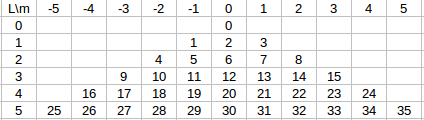
\includegraphics[width=0.5\linewidth]{Figures/jindex.png}
    \caption{Indices of $Y_j$ as a subset of $Y_{\ell m}$.}
    \label{fig:indices}
\end{figure}

\noindent With this convention we can recast equation \ref{eq:SNequations} using 

\begin{align*}
\phi_{mg'} = \sum_{n'=0}^{N}
w_{n'}
Y_{m}(\hat{\Omega}_n')
. \Psi_{g'n'}(r),
\end{align*}
and the notion that $\phi_{mg'} = \phi_{\ell m_{true}g'}$ for $m=\ell(\ell+2)+m_{true}-\ell$, as well as $\Sigma_{sm,g'{\to}g} = \Sigma_{sm_{true},g'{\to}g}$, to

\begin{equation} \label{eq:SNequationsSingleMOm}
\begin{aligned}
&\biggr(\hat{\Omega}_n\nabla +\Sigma_{tg} (r)\biggr)  \Psi_{gn} (r)\\
&=       
\sum_{m=0}^{m_{max}}
M_{m}(\hat{\Omega}_n)
\sum_{g'=0}^{G} \biggr[  
\Sigma_{sm,g'{\to}g} (r)
. \phi_{mg'}
\biggr]
+  Q_{fixed,g,n} (r).
\end{aligned}
\end{equation}
\newline
Where $M_m$ is developed from each $\ell,m_{true}$ pair to get
\begin{equation} \label{eq:rough_m2d}
\begin{aligned}
m=\ell(\ell+1)+ m_{true}\\
M_m(\hat{\Omega}_n) = M_{mn}= \frac{2\ell+1}{4\pi}Y_{\ell m}
\end{aligned}
\end{equation}

We now defined the notation $M_m(\hat{\Omega}_n)=M_{mn}$ and $Y_m (\hat{\Omega}_n) = Y_{mn}$, drop the notation $(r)$ for simplicity and rearrange the terms in equation \ref{eq:SNequationsSingleMOm} to get

\begin{equation} \label{eq:SNequationsSingleMOmReArr}
\begin{aligned}
\biggr(\hat{\Omega}_n\nabla +\Sigma_{tg} \biggr)  \Psi_{gn} 
=    \sum_{m=0}^{m_{max}}     
M_{mn}
.
\sum_{g'=0}^{G}
\biggr[
\Sigma_{sm,g'{\to}g} 
. \phi_{mg'}
\biggr]
+  Q_{fixed,g,n} (r).
\end{aligned}
\end{equation}
\newline
The summation over groups for a specific moment is known as a \textbf{source moment}, $q_{m,g}$, such that
\begin{equation} \label{eq:sourcemoment}
q_{m,g}=
\sum_{g'=0}^{G}
\biggr[
\Sigma_{sm,g'{\to}g} 
. \phi_{mg'}
\biggr]
\end{equation} 


\vspace{1.5cm}
\subsection{Operator form}
The streaming and removal terms can be denoted as $L$ such that

\begin{align*}
\biggr(\hat{\Omega}_n\nabla +\Sigma_{tg} \biggr)  \Psi_{gn}  = \mathbf{L}_{gn}\Psi_{gn} 
\end{align*}
\newline
We will now additionally cast the source terms into the form

\begin{align}
\sum_{m=0}^{m_{max}}     
M_{mn}
.
\sum_{g'=0}^{G}
\biggr[
\Sigma_{sm,g'{\to}g} 
. \phi_{mg'}
\biggr] \ 
+ \ S_{gn} (r) = \mathbf{M}_n \mathbf{S}_g \mathbf{D} \mathbf{\Psi} \ + \ Q_{fixed,g,n}
\end{align}

\noindent For the scattering source term we see that we have a Discrete-to-moment operator $\mathbf{D}^*$, resulting from the quadrature rule of integration over angle (with the $^*$ denoting a group independent non-block matrix), such that for a given moment $m$ we have
\begin{align*}
\phi_{mg'} &= 
\sum_{n'=0}^{N} w_{n'} . Y_{m n'}.\Psi_{g'n'} \\
&= \sum_{n'=0}^N D_{mn'}.\Psi_{g'n'} \\
&= 
\begin{bmatrix}
D_{m0} &\hdots  &D_{mN}\\
\end{bmatrix}
\begin{bmatrix}
\Psi_{g'0} \\
\vdots    \\
\Psi_{g'N}
\end{bmatrix}
\end{align*}

where $D_{mn'}=w_{n'}Y_{mn'}$.
When the components of all moments and angles are arranged in a matrix the flux moments for a particular group $g'$ are given by 
\begin{equation}
\begin{aligned}
\therefore
\boldsymbol{\phi}_{g'} &=  
\begin{bmatrix}
\phi_{0,g'} \\
\vdots \\
\phi_{m_{max},g'}
\end{bmatrix}=
\begin{bmatrix}
D_{00} &\hdots &D_{0N} \\
\vdots &\ddots &\vdots  \\
D_{m_{max}0} &\hdots &D_{mN}
\end{bmatrix}
\begin{bmatrix}
\Psi_{g'0} \\
\vdots    \\
\Psi_{g'N}
\end{bmatrix}\\
\therefore
\boldsymbol{\phi}_{g'}
&=\mathbf{D}^*\mathbf{\Psi}_{g'} 
\end{aligned}
\end{equation}

This form of the Discrete-to-moment operator is not conducive to computing the source moments as depicted in equation \ref{eq:sourcemoment}. To this end we duplicate each row of $\mathbf{D}^*$ a total $G$ times (the number of groups) as

\begin{equation} \label{eq:phivector}
\begin{aligned}
\boldsymbol{\phi}&=
\begin{bmatrix}
\phi_{0,0'} \\ \vdots \\ \phi_{0,G'} \\
\phi_{1,0'} \\ \vdots \\ \phi_{1,G'} \\
\vdots \\ \vdots \\
\phi_{m_{max},0'} \\ \vdots \\ \phi_{m_{max},G'} \\
\end{bmatrix}
=
\begin{bmatrix}
D_{00} &\hdots &D_{0N} \\
\vdots \\
D_{00} &\hdots &D_{0N} \\
D_{10} &\hdots &D_{1N} \\
\vdots \\
D_{10} &\hdots &D_{1N} \\
& \vdots & \\ & \vdots & \\
D_{m_{max}0} &\hdots &D_{m_{max}N} \\
\vdots \\
D_{m_{max}0} &\hdots &D_{m_{max}N} \\
\end{bmatrix}
\begin{bmatrix}
\Psi_{0'0} \\
\vdots    \\
\Psi_{G'N} \\
\Psi_{0'0} \\
\vdots    \\
\Psi_{G'N} \\
\vdots \\ \vdots \\
\Psi_{0'0} \\
\vdots    \\
\Psi_{G'N} \\
\end{bmatrix} \\
\boldsymbol{\phi}&=\mathbf{D}\mathbf{\Psi}
\end{aligned}
\end{equation}

We now also add the scattering operator elements $S_{m,g'{\to}g}=\Sigma_{sm,g'{\to}g}$, a diagonal matrix used to construct the source moments such that
\begin{align}
q_{m,g}&=
\sum_{g'=0}^{G}
\biggr[
\Sigma_{sm,g'{\to}g} 
. \phi_{mg'}
\biggr] 
= 
\begin{bmatrix}
S_{m,0'{\to}g} &\hdots &S_{m,G'{\to}g}
\end{bmatrix} \boldsymbol{\phi}_{g'} 
\end{align}
and when arranged in the same moment-then-group indexes used for the flux moments we obtain, for a group $g$ the form of the source moments $\mathbf{Q}_{mom,g}$ and the scattering operator $\mathbf{S}_g$ from

\begin{equation}
\begin{aligned}
\mathbf{Q}_{mom,g}&=
\begin{bmatrix}
q_{0,g} \\ 
\vdots \\
q_{m_{max},g} \\
\end{bmatrix}
=
\begin{bmatrix}
&S_{0,0'{\to}g} \hdots S_{0,G'{\to}g} 
&0\hdots 0 
&0\hdots 0 
&0\hdots 0\\
&0 \hdots 0  
&S_{1,0'{\to}g} \hdots S_{1,G'{\to}g}
&\hdots 
&\vdots \\
&\vdots 
&\hdots 
&\ddots 
&\vdots \\
&0 
&\hdots 
&\hdots
&S_{m_{max},0'{\to}g} \hdots S_{m_{max},G'{\to}g}
\end{bmatrix}
\mathbf{D}\mathbf{\Psi} \\
\therefore
\mathbf{Q}_{mom,g}
&=
\mathbf{S}_g\mathbf{D}\mathbf{\Psi}.
\end{aligned}
\end{equation}
\newline
This portion of the computation is an import part of the simulation sequence since it forms the basic building block of source iteration. It is also part of the last step before the source to a single angular direction is computed. A separate routine is normally employed to compute the group aggregated source moments $\mathbf{Q}_{mom}$ as

\begin{align}
\mathbf{Q}_{mom} = 
\begin{bmatrix}
\mathbf{Q}_{mom,0} \\
\vdots \\
\mathbf{Q}_{mom,G}
\end{bmatrix}
\end{align}
\newline
Upon solving for a particular direction $n$ and group $g$ the source moment contribution to a particular direction is performed using the per-angle Moment-to-discrete operator, $\mathbf{M}_n$, with elements $M_{mn}$ defined in equation \ref{eq:rough_m2d} and takes the form 

\begin{align*}
\sum_{m=0}^{m_{max}}M_{mn} \mathbf{Q}_{mom,g}
&= 
\begin{bmatrix}
M_{0,n} &\hdots &M_{m_{max},n}
\end{bmatrix}
\mathbf{Q}_{mom,g} \\
&= \mathbf{M}_n \mathbf{S}_g \mathbf{D} \mathbf{\Psi}
\end{align*}
\newline
This now completes our casting to operator form for a specific angle
\begin{align}
\mathbf{L}_{gn}\Psi_{gn} = \mathbf{M}_n \mathbf{S}_g \mathbf{D} \mathbf{\Psi} \ + \ Q_{fixed,g,n}
\end{align}
\newline
The final level of operator-form is the angle and group aggregated form. The streaming operator $\mathbf{L}$ is a block diagonal matrix arranged by groups then angles. The $\mathbf{\Psi}$ vector is the same as the one defined in equation \ref{eq:phivector}. Since the in-scattering sources and fixed sources are already scalar values for a given group and angle, they too become just vectors. 

\begin{equation}
\begin{aligned}
\mathbf{L} = 
\begin{bmatrix}
&\mathbf{L}_{00} 
&\hdots  
&\hdots 
&[0] \\
&\vdots
&\mathbf{L}_{10}
&\hdots
&\vdots \\
&\vdots 
&\hdots 
&\ddots 
&\vdots \\
&[0]
&\hdots 
&\hdots 
&\mathbf{L}_{GN} 
\end{bmatrix}
\end{aligned}
\end{equation}
\begin{equation}
\begin{aligned}
\mathbf{MSD} = 
\begin{bmatrix}
&\mathbf{M}_0\mathbf{S}_0\mathbf{D} \\
&\mathbf{M}_0\mathbf{S}_1\mathbf{D} \\
&\vdots \\
&\mathbf{M}_N\mathbf{S}_G\mathbf{D} \\
\end{bmatrix}
\end{aligned}
\end{equation}
\begin{equation}
\begin{aligned}
\mathbf{Q}_{fixed} = 
\begin{bmatrix}
&Q_{fixed,0,0} \\
&Q_{fixed,1,0} \\
&\vdots \\
&Q_{fixed,G,N} \\
\end{bmatrix}
\end{aligned}
\end{equation}
\newline
Finally we have the operator form

\begin{align} \label{eq:NTEoperatorform}
\mathbf{L}\Psi 
= \mathbf{M} \mathbf{S} \mathbf{D} \Psi \
+ \ \mathbf{Q}_{fixed}
\end{align}




\subsection{No scattering - Computing the fixed source}
With no scattering the discrete problem to solve per cell is 
\begin{align*}
\mathbf{L}_{gn}\Psi_{gn} 
= 
s_{gn} \\
\Psi_{gn} 
= 
\mathbf{L}_{gn}^{-1} s_{gn} 
\end{align*}
and can be solved by sweeping along the direction of each angle. Suppose we store the angular flux then per cell and sweep through all angles. We can then obtain the scalar flux from
\begin{align*}
\phi = \mathbf{D}\Psi
= 
\mathbf{D}\mathbf{L}^{-1} s.
\end{align*}
However, the storage of the angular flux is prohibitively expensive, and therefore we have to look at the moment-by-moment accumulation of the scalar flux moments. First we can look again at 
\begin{align*}
\sum_{n=0}^{N} w_{n} . Y_{mn}.\Psi_{gn}
= 
\begin{bmatrix}
w_0 Y_{m0} &\hdots  &w_{N} Y_{mN}\\
\end{bmatrix}
\begin{bmatrix}
\Psi_{g0} \\
\vdots    \\
\Psi_{gN}
\end{bmatrix}
=\mathbf{D}_m\Psi_{g}(r) =\phi_{mg}.
\end{align*}
This equation hints at the possibility of \textit{accumulating} the scalar flux by starting with the first angle
$$\phi_{mg}^{new}=0+w_0 Y_{m0}\Psi_{g0}$$
and thereafter
$$\phi_{mg}^{new}=\phi_{mg}^{old}+w_n Y_{m n}\Psi_{gn}.$$
In this fashion we only ever have to store the scalar flux moments in each cell. For fixed source problems, it can be advantageous to call this step the \textit{fixed source caculation} since it does not change when adding scattering or reaction based neutron source.


\subsection{With scattering - Computing the scattering source (Richardson Iteration)}
The addition of a scattering source, or for that matter a reaction based neutron source like fission, transforms the problem into an implicit system of equations to solve. The reason for this is that the scattering source requires a flux driver ... one we don't have at the start of the problem. To this end we manipulate our transport equation as follows:
\begin{align*}
\mathbf{L}\Psi 
&= \mathbf{M} \mathbf{S} \mathbf{D} \Psi
+s \\
\Psi &= \mathbf{L}^{-1} \mathbf{MSD}\Psi + \mathbf{L}^{-1} s \\
 \mathbf{D}\Psi &=  \mathbf{D}\mathbf{L}^{-1} \mathbf{MSD}\Psi +  \mathbf{D}\mathbf{L}^{-1} s \\
 \therefore
\phi &= \mathbf{D}\mathbf{L}^{-1} \mathbf{MS}\phi +  \mathbf{D}\mathbf{L}^{-1} s
\end{align*}

One solution to this form of the problem is: when we are computing $\phi$ at iteration $\ell$ (i.e. $\phi^{(\ell)}$) we can approximate the scattering source from the previous iteration's $\phi$ (i.e. $\phi^{(\ell-1)}$) which leads to 
\begin{align*}
\phi^{(\ell)} &= \mathbf{D}\mathbf{L}^{-1} \mathbf{MS}\phi^{(\ell-1)} +  \mathbf{D}\mathbf{L}^{-1} s.
\end{align*}
This form is known as \textbf{Richardson Iteration}.


\newpage
\chead{Application of the Finite Element Method}
\section{Application of the Finite Element Method}
The lower triangular operator $\mathbf{L}$ in equation \ref{eq:NTEoperatorform} is the operator to a hyperbolic partial differential equation for which an effective method to spatially discretize in space is the Discontinuous Galerkin method (DG). There are two well known methods for constructing the basis functions for the DG-method, one is the use of shape functions defined on a node and connecting to all nodes, across reference elements, of subscribing cells and when defined as linear functions these are called Piece-Wise Linear shape functions. The other method is the use of Linear Discontinuous shape functions which will not be discussed here. We shall refer to the Discontinous Galerkin method with the use of Piece-wise Linear basis functions as PWLD for further discussions.
\newline 
\newline
To see where this fits into the finite element method we consider a simple first order partial differential equation
\beqn 
\Omega \bigcdot \nabla \Psi + \sigma \Psi= q.
\eeqn 

For each node we multiply by the (not yet defined) trial space $\tau_i$ and require that 

\beq
\int_V \biggr[ \tau_i \Omega \bigcdot \nabla \Psi + \sigma \tau_i \Psi  -\tau_i q \biggr].dV = 0.
\eeq
\beqn
\therefore
\int_V\tau_i \Omega \bigcdot  \nabla \Psi .dV+ \int_V \sigma \tau_i \Psi.dV  -\int_V\tau_i q .dV= 0.
\eeqn 
Applying integration by parts for the first term results in 

\beqn
\int_V \Omega \bigcdot \nabla (\tau_i \Psi).dV  - \int_V  \Psi \Omega \bigcdot \nabla \tau_i.dV + \int_V \sigma \tau_i \Psi.dV-\int_V\tau_i q .dV= 0
\eeqn 

where we can apply Gauss's divergence theorem to the first term to obtain

\beqn
\int_{\partial V} (\Omega \bigcdot \hat{n}) \tau_i \Psi.dS  - \int_V \Psi \Omega \bigcdot  \nabla \tau_i.dV+ \int_V \sigma \tau_i \Psi.dV-\int_V\tau_i q .dV= 0.
\eeqn 

We now apply an upwinding scheme to the boundary integral 

\beq
\int_{\partial V} (\Omega \bigcdot \hat{n}) \tau_i \tilde{\Psi}.dS  - \int_V \Psi \Omega \bigcdot  \nabla \tau_i.dV+ \int_V \sigma \tau_i \Psi.dV-\int_V\tau_i q .dV= 0.
\eeq 
where
\beqn
\tilde{\Psi} =
\begin{cases}
\Psi_{within cell} \quad \quad &\text{if } \hat{n}\bigcdot \Omega > 0 \\
\Psi_{upwind cell} \quad \quad &\text{if } \hat{n}\bigcdot \Omega < 0 \\
\end{cases}
\eeqn 

We now apply integration again to the second term

\beq
\int_{\partial V} (\Omega \bigcdot \hat{n}) \tau_i \tilde{\Psi}.dS  
- \int_V \Omega \bigcdot  \nabla (\tau_i \Psi ) .dV 
+\int_V \tau_i \Omega \bigcdot  \nabla \Psi .dV+ \int_V \sigma \tau_i \Psi.dV-\int_V\tau_i q .dV= 0.
\eeq 

and then Gauss's divergence theorem again on the second term of this

\beq
\int_{\partial V} (\Omega \bigcdot \hat{n}) \tau_i (\tilde{\Psi} - \Psi).dS  
+\int_V \tau_i \Omega \bigcdot  \nabla \Psi .dV+ \int_V \sigma \tau_i \Psi.dV-\int_V\tau_i q .dV= 0.
\eeq 

Now, when we expand $\Psi$ into basis functions, with the basis functions $b_j$ essentially being the same as the trial functions $\tau_i$ (i.e. when $i=j$), as 
$$
\Psi = \sum_{j=0}^{N_{dof}-1} b_j \Psi_j
$$
we arrive at the ``per DOF" version of the finite element equation

\beqn \label{eq:finiteelement2Dtriangle}
 \sum_{j=0}^{N_{dof}-1}
 \biggr[
\int_{\partial V} (\Omega \bigcdot \hat{n}) \tau_i (\tilde{\Psi} - \Psi_j.b_j).dS  
+\int_V \Psi_j \tau_i \Omega \bigcdot  \nabla b_j .dV
+ \int_V \Psi \sigma \tau_i b_j.dV
 \biggr]= \int_V\tau_i q .dV.
\eeqn 
\newline
From this equation we see that we need expressions for the shape function $\tau_i$ and $b_j$ as well as the derivative of the trial function $\nabla \tau_i$. We also need a means to efficiently integrate these functions over surface and volume.
\newline
\newline
Given the discontinuous nature of this formulation we can solve the set of trial spaces $\tau_i$ associated with a given cell provided that the upstream fluxes are known. This gives rise to the concept of the \textbf{sweep} where the transport operator $\mathbf{L}$ is inverted cell-by-cell in the order of dependencies.


\newpage
\chead{Application of piecewise linear shape functions}
\section{Application of piecewise linear shape functions}

\subsection{Piecewise linear shape functions on a 2D triangle}
For a two dimensional simulation using triangular elements we seek to map a triangle in cartesian space to a reference triangle in natural coordinates. We do this because we can develop a method to perform integration or differentation for the reference triangle that can be mapped to a triangle of any shape and location. An example of the two triangles in different coordinate space is shown in Figure \ref{fig:twodreferenceelement}.

\begin{figure}[H]
\centering
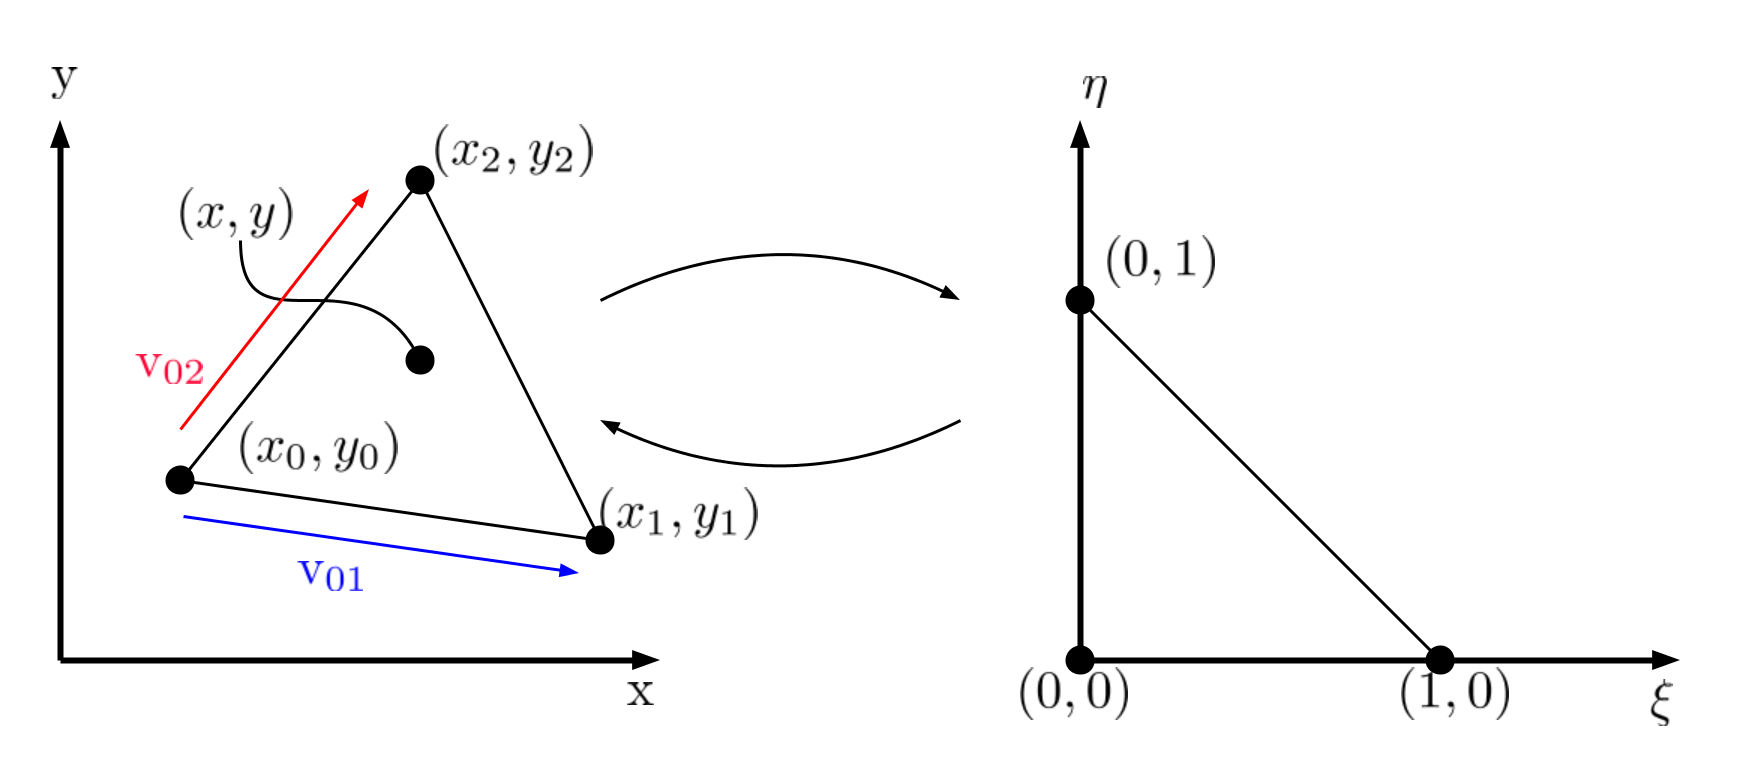
\includegraphics[width=0.8\linewidth]{LatexDraw/TwoD_ReferenceElement}
\caption{Mapping of a 2D triangle to a reference triangle in natural coordinates.}
\label{fig:twodreferenceelement}
\end{figure}

The linear basis functions for the reference triangle are

\beq 
N_0(\xi,\eta) &= 1 - \xi - \eta \\
N_1(\xi,\eta) &= \xi \\
N_2(\xi,\eta) &= \eta. \\
\eeq 
From these functions we can interpolate the point $(x,y)$ with the following

\beq 
x &= N_0 x_0 + N_1 x_1 + N_2 x_2 \\
y &= N_0 y_0 + N_1 y_1 + N_2 y_2 \\
\eeq 
We can now express $x$ and $y$ as functions of $\xi$ and $\eta$ by substituting the expressions for $N_0$, $N_1$ and $N_2$ into the expressions for $x$ and $y$

\beq 
x &= (1-\xi-\eta)x_0 + (\xi)x_1 + (\eta)x_2 \\
&= x_0 -\xi x_0 -\eta x_0 +\xi x_1 +\eta x_2 \\
&= x_0 +(x_1 - x_0)\xi + (x_2 - x_0)\eta
\eeq 
and
\beq 
y &= (1-\xi-\eta)y_0 + (\xi)y_1 + (\eta)y_2 \\
&= y_0 -\xi y_0 -\eta y_0 +\xi y_1 +\eta y_2 \\
&= y_0 +(y_1 - y_0)\xi + (y_2 - y_0)\eta
\eeq 
\newline
In terms of the vectors from vertex $0$ to the other two vertices (refer to Figure \ref{fig:twodreferenceelement}) we can write this as

\beqn \label{eq:x2Dnat}
x = x_0 + \text{v}_{01x} \xi +\text{v}_{02x} \eta
\eeqn 
\beqn \label{eq:y2Dnat}
y = y_0 + \text{v}_{01y} \xi +\text{v}_{02y} \eta
\eeqn 
\newline
which is in the form of a linear transformation and from which we can determine the very important Jacobian matrix

\begingroup
\renewcommand*{\arraystretch}{1.5}
\beqn \label{eq:jacobiantriangle} 
\mathbf{J }= 
\begin{bmatrix}
\dfrac{dx}{d\xi}     & \dfrac{dx}{d\eta} \\
\dfrac{dy}{d\xi}     & \dfrac{dy}{d\eta} \\
\end{bmatrix}=
\begin{bmatrix}
\text{v}_{01x}  & \text{v}_{02x}  \\
\text{v}_{01y}  & \text{v}_{02y}  \\
\end{bmatrix}
=
\begin{bmatrix}
(x_1 - x_0) & (x_2 - x_0)  \\
(y_1 - y_0)  & (y_2 - y_0) \\
\end{bmatrix}.
\eeqn
\endgroup
\newline
The first application of the Jacobian will be for the integration of the trial or basis function in the finite element method. For simplicity let us consider the integration of a function over $x$ and $y$ which can be transformed to an integration of the linear transformation of function f, i.e. function g, over $\xi$ and $\eta$ using fundamental linear algebra. This integration is then

\beq 
\int \int f(x,y) .dx.dy = \int \int g (\xi,\eta).|J|.d\xi.d\eta
\eeq 
\newline
where $|J|$ is the determinant of the Jacobian. This integration can then easily be done either analytically or by using a quadrature rule. For the reference triangle this can easily be done using the method of undetermined coefficients as detailed in appendix \ref{appendix:trianglequadrature}.
\newline
\newline 
We need to define one more item that is related to the finite element method and that is the derivative of the basis functions, $\nabla N_i(\xi,\eta)$, which can be developed by noting that

\beq 
\frac{\partial N_i}{\partial \xi} = 
\frac{\partial N_i}{\partial x}\cdot \frac{\partial x}{\partial \xi} \ + \ 
\frac{\partial N_i}{\partial y}\cdot  \frac{\partial y}{\partial \xi}
\eeq 
\beq 
\frac{\partial N_i}{\partial \eta} = 
\frac{\partial N_i}{\partial x}\cdot \frac{\partial x}{\partial \eta} \ + \ 
\frac{\partial N_i}{\partial y}\cdot  \frac{\partial y}{\partial \eta}
\eeq 
\newline
which can be written as

\begingroup
\renewcommand*{\arraystretch}{1.5}
\beq
\begin{bmatrix}
\dfrac{\partial N_i}{\partial \xi} \\
\dfrac{\partial N_i}{\partial \eta}
\end{bmatrix}
&=
\begin{bmatrix}
\dfrac{\partial x}{\partial \xi}   &\dfrac{\partial y}{\partial \xi} \\
\dfrac{\partial x}{\partial \eta}   &\dfrac{\partial y}{\partial \eta} \\
\end{bmatrix}
\begin{bmatrix}
\dfrac{\partial N_i}{\partial x} \\
\dfrac{\partial N_i}{\partial y}
\end{bmatrix} \\
\therefore 
\begin{bmatrix}
\dfrac{\partial N_i}{\partial \xi} \\
\dfrac{\partial N_i}{\partial \eta}
\end{bmatrix}
&= \mathbf{J}^T 
\begin{bmatrix}
\dfrac{\partial N_i}{\partial x} \\
\dfrac{\partial N_i}{\partial y}
\end{bmatrix}.
\eeq 
\endgroup

Now we can invert $\mathbf{J}^T$ to get

\begingroup
\renewcommand*{\arraystretch}{1.5}
\beqn \label{eq:derivativeNtriangle}
\begin{bmatrix}
\dfrac{\partial N_i}{\partial x} \\
\dfrac{\partial N_i}{\partial y}
\end{bmatrix}
&=
(\mathbf{J}^T)^{-1}
\begin{bmatrix}
\dfrac{\partial N_i}{\partial \xi} \\
\dfrac{\partial N_i}{\partial \eta}
\end{bmatrix}
\eeqn 
\endgroup

and since the inverse of a $2\stimes 2$ matrix is given by

\beq 
\begin{bmatrix}
a & b\\
c & d
\end{bmatrix}^{-1}
=\frac{1}{ad-bc} 
\begin{bmatrix}
d & -b\\
-c & a
\end{bmatrix}
\eeq 

we have

\begingroup
\renewcommand*{\arraystretch}{1.5}
\beqn \label{eq:jacobianinversetriangle}
(\mathbf{J}^T)^{-1} =
\begin{bmatrix}
\dfrac{\partial x}{\partial \xi}   &\dfrac{\partial y}{\partial \xi} \\
\dfrac{\partial x}{\partial \eta}   &\dfrac{\partial y}{\partial \eta} \\
\end{bmatrix}^{-1}
&=
\frac{1}{|J|}
\begin{bmatrix}
\dfrac{\partial y}{\partial \eta}   & -\dfrac{\partial y}{\partial \xi} \\
-\dfrac{\partial x}{\partial \eta}  & \dfrac{\partial x}{\partial \xi} 
\end{bmatrix}
\eeqn
\endgroup


\newpage
\textbf{In summary:}\newline 
In two dimensions using triangular cells, we wish to represent equation \ref{eq:finiteelement2Dtriangle} (repeated here)

\beq
 \sum_{j=0}^{N_{dof}-1}
 \biggr[
\int_{\partial V} (\Omega \bigcdot \hat{n}) \tau_i (\tilde{\Psi} - \Psi_j.b_j).dS  
+\int_V \Psi_j \tau_i \Omega \bigcdot  \nabla b_j .dV
+ \int_V \Psi \sigma \tau_i b_j.dV
 \biggr]= \int_V\tau_i q .dV.
\eeq
\newline
where $\tau_i(\xi,\eta) = b_i(\xi,\eta) = N_i(\xi,\eta)$, the latter being the shape functions for each of the vertices of a triangular cell. We can evaluate these shape functions at any value of $\xi$ and $\eta$ within the reference triangle shown in Figure \ref{fig:twodreferenceelement} as

\beq 
N_0(\xi,\eta) &= 1 - \xi - \eta \\
N_1(\xi,\eta) &= \xi \\
N_2(\xi,\eta) &= \eta. \\
\eeq 
\newline
The derivatives of the shape functions $\nabla \tau_i(\xi,\eta) = \nabla b_i(\xi,\eta) = \nabla N_i(\xi,\eta)$ can be computed with a given triangle using equations \ref{eq:derivativeNtriangle}, \ref{eq:jacobianinversetriangle} and \ref{eq:jacobiantriangle}, repeated respectively here

\begingroup
\renewcommand*{\arraystretch}{1.5}
\beq
\begin{bmatrix}
\dfrac{\partial N_i}{\partial x} \\
\dfrac{\partial N_i}{\partial y}
\end{bmatrix}
&=
(\mathbf{J}^T)^{-1}
\begin{bmatrix}
\dfrac{\partial N_i}{\partial \xi} \\
\dfrac{\partial N_i}{\partial \eta}
\end{bmatrix}
\eeq 
\endgroup

\begingroup
\renewcommand*{\arraystretch}{1.5}
\beq
(\mathbf{J}^T)^{-1} =
\begin{bmatrix}
\dfrac{\partial x}{\partial \xi}   &\dfrac{\partial y}{\partial \xi} \\
\dfrac{\partial x}{\partial \eta}   &\dfrac{\partial y}{\partial \eta} \\
\end{bmatrix}^{-1}
&=
\frac{1}{|J|}
\begin{bmatrix}
\dfrac{\partial y}{\partial \eta}   & -\dfrac{\partial y}{\partial \xi} \\
-\dfrac{\partial x}{\partial \eta}  & \dfrac{\partial x}{\partial \xi} 
\end{bmatrix}
\eeq
\endgroup

\begingroup
\renewcommand*{\arraystretch}{1.5}
\beq
\mathbf{J }= 
\begin{bmatrix}
\dfrac{dx}{d\xi}     & \dfrac{dx}{d\eta} \\
\dfrac{dy}{d\xi}     & \dfrac{dy}{d\eta} \\
\end{bmatrix}=
\begin{bmatrix}
\text{v}_{01x}  & \text{v}_{02x}  \\
\text{v}_{01y}  & \text{v}_{02y}  \\
\end{bmatrix}
=
\begin{bmatrix}
(x_1 - x_0) & (x_2 - x_0)  \\
(y_1 - y_0)  & (y_2 - y_0) \\
\end{bmatrix}.
\eeq
\endgroup

Integrals of the form 
\beq 
&\int_V \tau_i b_j .dV   \quad \quad \text{and } &&\int_V \tau_i \Omega \bigcdot \nabla b_j .dV
   \quad \quad \text{and } && \int_V \tau_i .dV
\eeq 
can now be evaluated using a quadrature rule of the form
\beq 
\int_V f(x,y) .dx.dy = \int_{-1}^1 \int_0^{1-\eta} g(\xi,\eta).|J|.d\xi.d\eta = |J| \sum_{q=0}^{N_q-1} w_q g(\xi_q,\eta_q)
\eeq 
where the quadrature weights and points are given in appendix \ref{appendix:trianglequadrature} and $g(\xi,\eta)$ are combinations of the basis functions $N_i$. Note the dot-product where the derivative of the base function is used. Also note that the derivative of the basis function results in a vector.




\newpage 
\subsection{Piecewise linear shape functions on a 2D polygon}
The development of the methodology as applied to a 2D triangle has direct application when applied to a polygon since a polygon most
 likely presents more complexity than classical reference elements like quadrilaterals and therefore using triangles as grp\_subsets of polygons overcomes this complexity. The use of subset triangles for the representation of a polygon was presented by Bailey \& Adams in \cite{BaileyAdamsPWLPolygons} the same authors which subsequently studied bi-linear basis functions \cite{BaileyAdamsPWBLPolygons}. From the latter paper it is this author's judgement that bi-linear basis functions offer little benefit over their linear counterparts and we will therefore pursue the linear methods presented in \cite{BaileyAdamsPWLPolygons}. The basis functions for each vertex of a polygon are of the form

\beqn 
P_i(x,y) = N_i(x,y) + \beta_i N_c(x,y)
\eeqn 
\newline
where the functions $N_i$ and $N_c$ are the standard linear functions defined on triangles. The subscripts $i$ and $c$ refer to the vertices $i$ and center of the polygon, respectively. The $\beta_i$ value is a weighting constant defined such that 

\beqn 
\begin{bmatrix}
x \\ y
\end{bmatrix}_{c}
= \sum_{s=0}^{N_{s}} \beta_s 
\begin{bmatrix}
x \\ y
\end{bmatrix}_{s,avg}.
\eeqn
\newline
Naturally it follows that $\beta_s = \dfrac{1}{N_{s}}$ where $N_s$ is the amount of sides. $[x \ y]_{s,avg}$ is the average coordinate of the two vertices of a side. An example basis function is shown in Figure \ref{fig:twodpolygon}. It should be noted that a single basis function now requires integration on each of the sub-triangles of the polygon instead of just a single one.

\begin{figure}[H]
\centering
\includegraphics[width=0.5\linewidth]{LatexDraw/TwoD_Polygon}
\caption{Basis function on a 2D polygon.}
\label{fig:twodpolygon}
\end{figure}


It is hard to visualize that this approach leads to an equivalent representation but with a few tests one can establish that this is equivalent. Some aspects of the paper presenting this method \cite{BaileyAdamsPWLPolygons} that are not intuitive is the explanation that integration is now over all sides. Also, the paper does not explicitly state that the cell centroid never features as an unknown in the solution. The customary assembly of the matrix in triangle or quadrilateral based meshes is to assemble cell-by-cell with an inner loop over the DOF of the cell. This approach is essentially the same but the paper states that integration is per side without saying that each DOF (except the cell center) of each side is also an inner loop of this integration. The subtle differences in the two algorithms can be seen in algorithm \ref{algo:triangle} and \ref{algo:polygon}.
\newline
\newline
The method is versatile enough to applied to triangles and quadrilaterals where examples of the shape functions are shown in Figure

\begin{figure}[H]
\centering
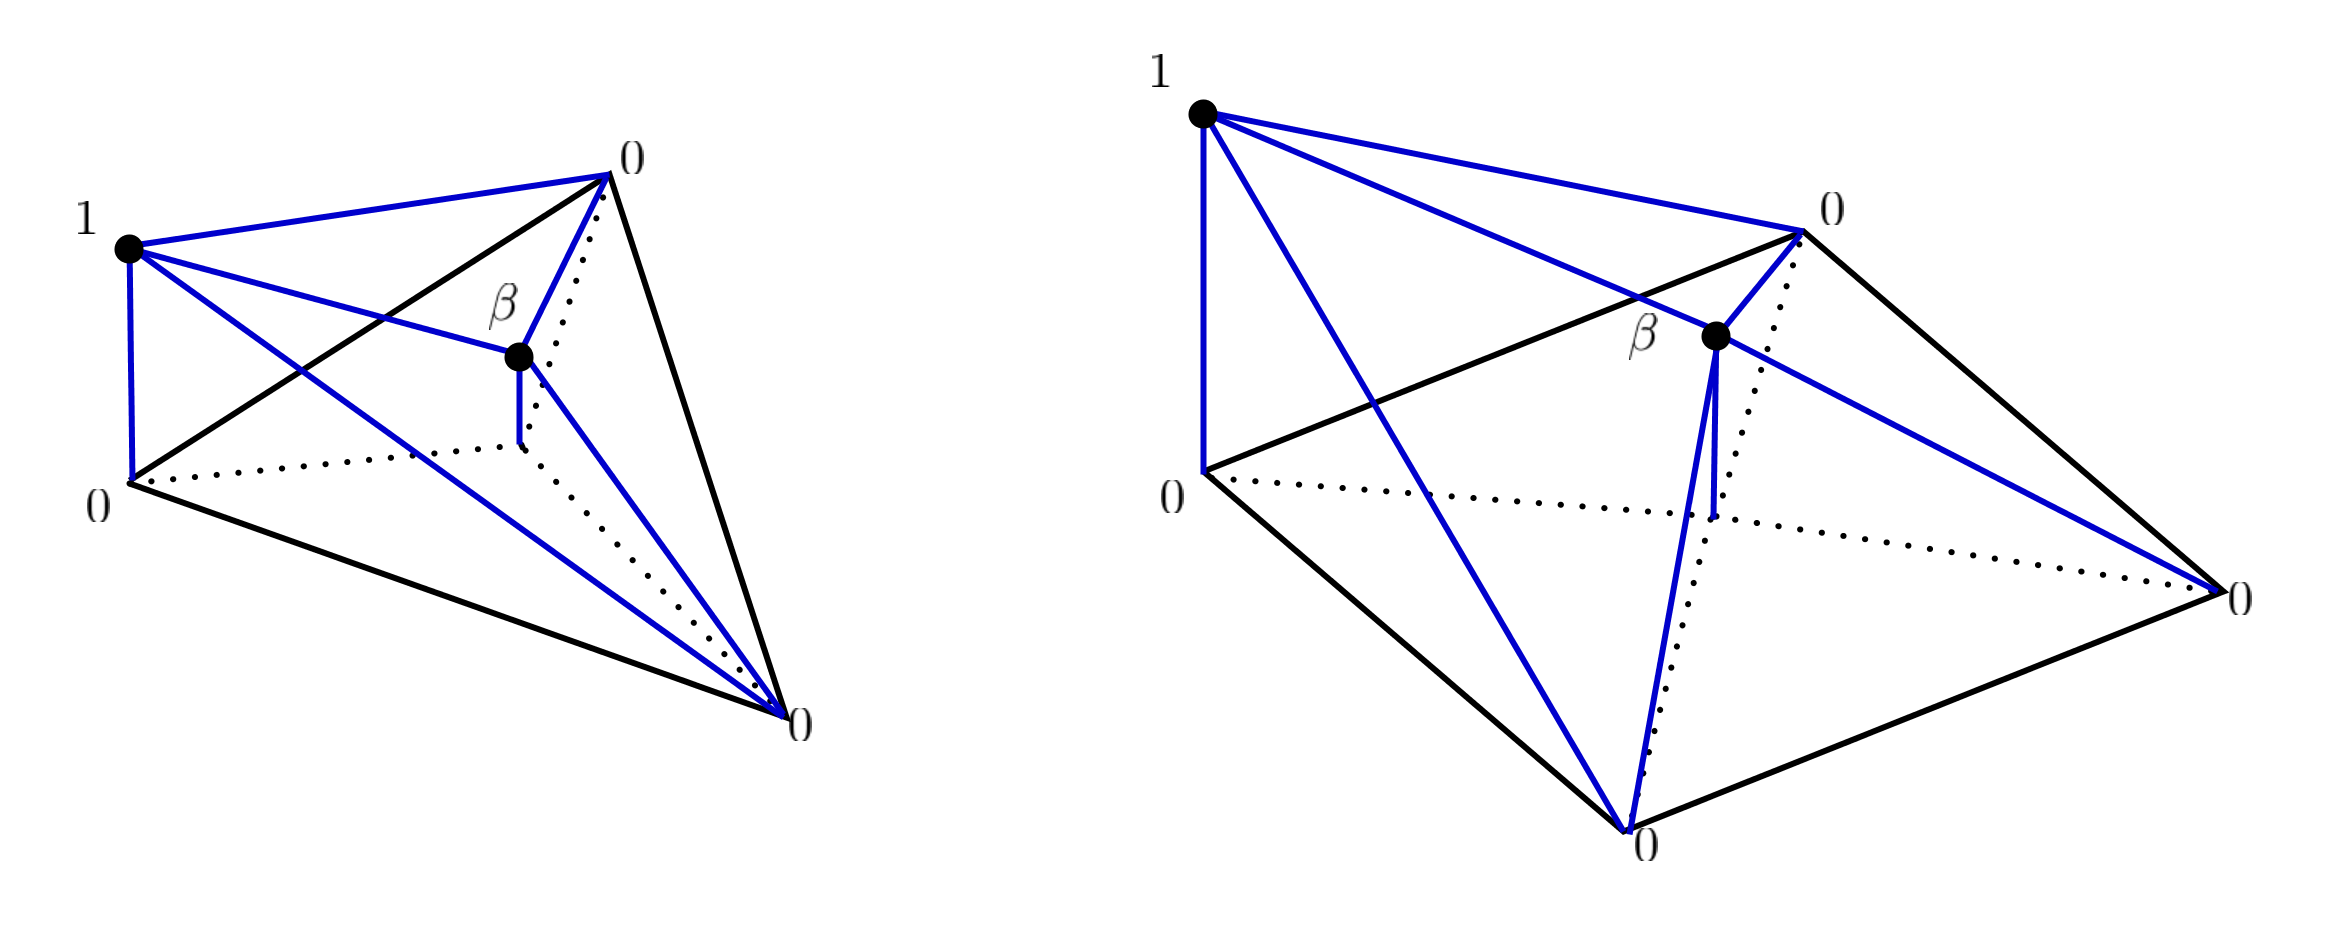
\includegraphics[width=1.0\linewidth]{LatexDraw/TwoD_PolygonTriQuad}
\caption{Basis functions on a triangle and on a quadrilateral.}
\label{fig:twodpolygontriquad}
\end{figure}


\vspace{0.5cm}
\begin{algorithm}[H]
\ForEach{cell}{
$A^{N_v\stimes N_v}$ $\longleftarrow$ Initialize matrix \;
$b^{N_v\stimes 1}$ $\longleftarrow$ Initialize right hand side \;
\ForEach{vertex $i$}{
\ForEach{vertex $j$}{
\ForEach{quadrature point qp}{
$a_{ij}=a_{ij} + $ $\longleftarrow$ Eq. with $\tau_i$ and $b_j$ integrated over cell\;
$b_i = b_i +$ $\longleftarrow$ Eq. with $\tau_i$ and $b_j$ integrated over cell\;
}
}
}
$\phi$ $\longleftarrow$ Solve system\;
}
\caption{Triangle Based algorithm\label{algo:triangle}}
\end{algorithm}

\vspace{0.5cm}
\begin{algorithm}[H]
\ForEach{cell}{
$A^{N_v\stimes N_v}$ $\longleftarrow$ Initialize matrix \;
$b^{N_v\stimes 1}$ $\longleftarrow$ Initialize right hand side \;
\ForEach{vertex $i$}{
\ForEach{vertex $j$}{
\ForEach{sub-triangle s}{
\ForEach{quadrature point qp}{
$a_{ij}=a_{ij} + $ $\longleftarrow$ Eq. with $\tau_i$ and $b_j$ integrated over sub-triangle\;
$b_i = b_i +$ $\longleftarrow$ Eq. with $\tau_i$ and $b_j$ integrated over sub-triangle\;
}
}
}
}
$\phi$ $\longleftarrow$ Solve system\;
}
\caption{Polygon Based algorithm\label{algo:polygon}}
\end{algorithm}




\newpage
\subsection{Piecewise linear shape functions on a 3D tetrahedron}
For a three dimensional simulation using tetrahedral elements we seek to map a tetrahedron in cartesian space to a reference tetrahedron in natural coordinates. We do this because we can develop a method to perform integration or differentation for the reference tetrahedron that can be mapped to a tetrahedron of any shape and location. An example of the two tetrahedron in different coordinate space is shown in Figure \ref{fig:threedreferenceelement}.

\begin{figure}[H]
\centering
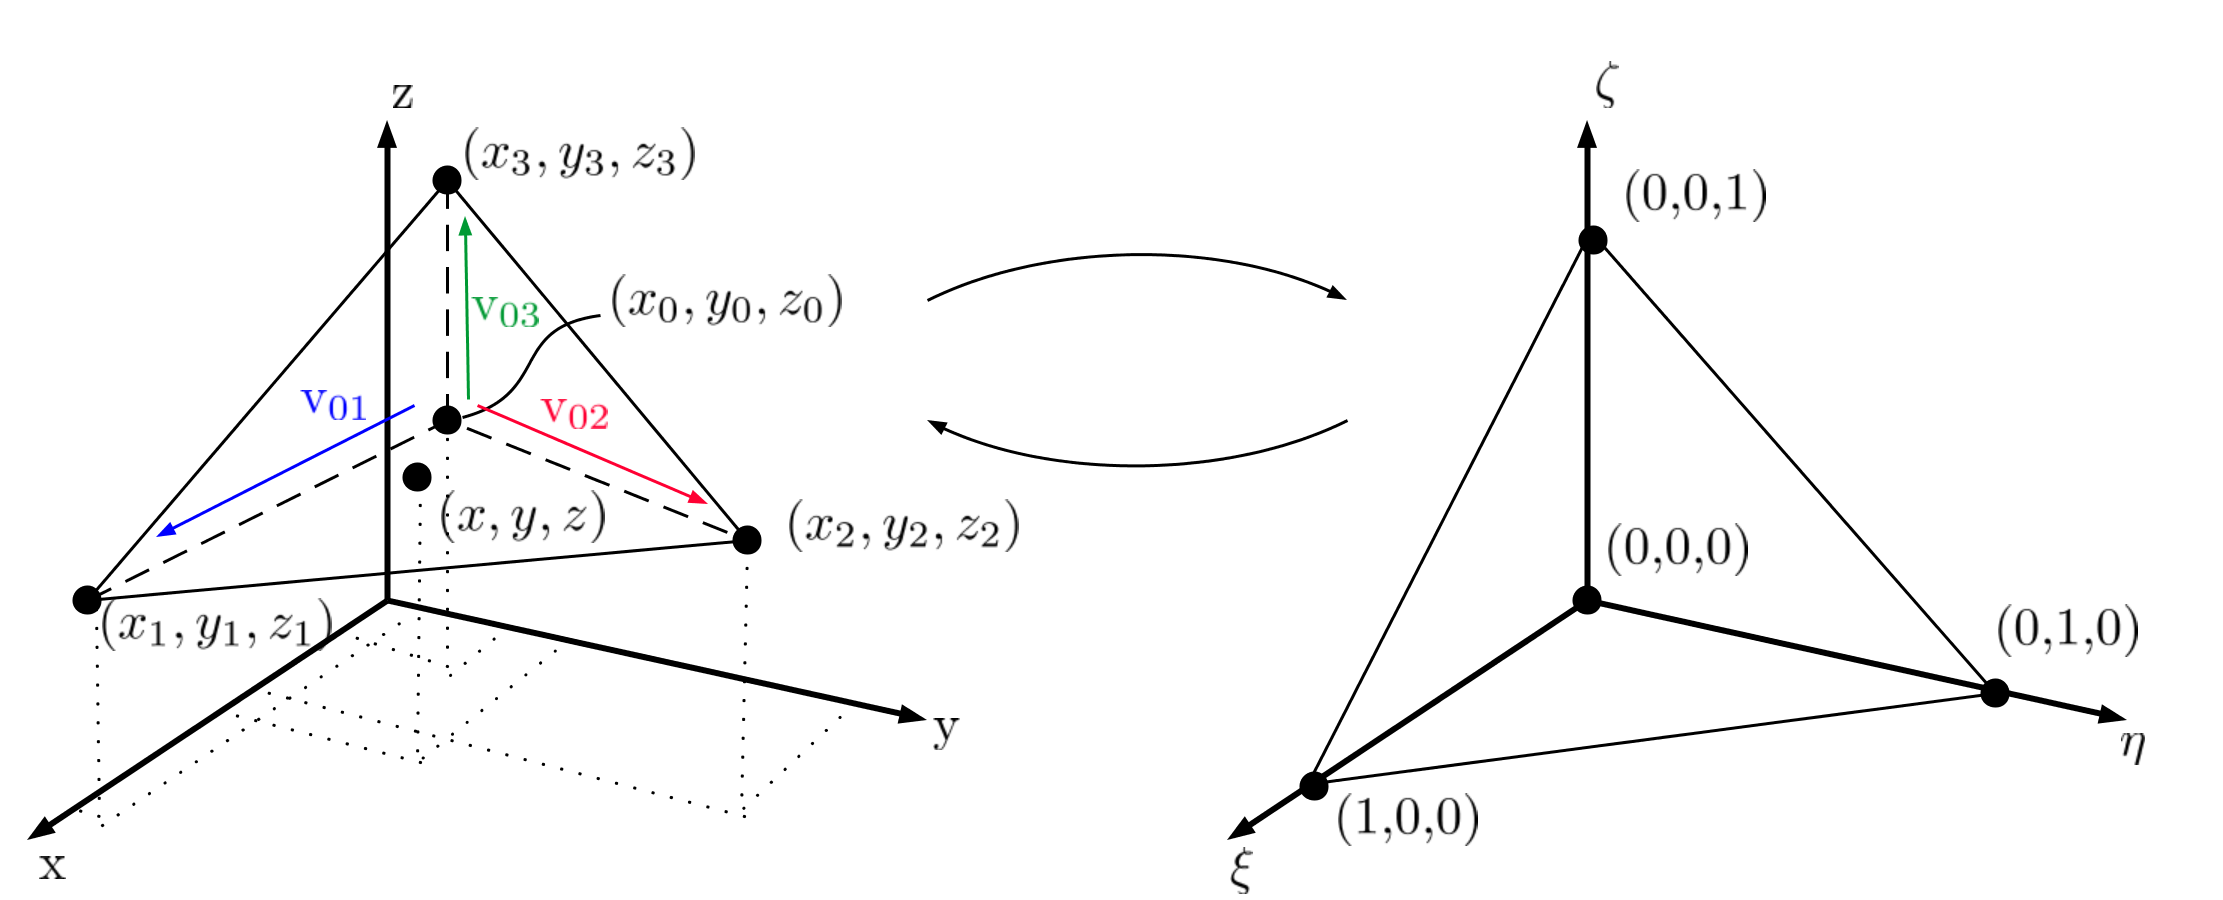
\includegraphics[width=1\linewidth]{LatexDraw/ThreeD_ReferenceElement}
\caption{Mapping of a 3D tetrahedron to a reference tetrahedron in natural coordinates.}
\label{fig:threedreferenceelement}
\end{figure}

The linear basis functions for the reference tetrahedron are

\beq 
N_0(\xi,\eta,\zeta) &= 1 - \xi - \eta - \zeta \\
N_1(\xi,\eta,\zeta) &= \xi \\
N_2(\xi,\eta,\zeta) &= \eta \\
N_3(\xi,\eta,\zeta) &= \zeta \\
\eeq 

From these functions we can interpolate the point $(x,y,z)$ with the following

\beq 
x &= N_0 x_0 + N_1 x_1 + N_2 x_2 + N_3 x_3 \\
y &= N_0 y_0 + N_1 y_1 + N_2 y_2 + N_3 y_3 \\
z &= N_0 z_0 + N_1 z_1 + N_2 z_2 + N_3 z_3 \\
\eeq 
\newline
We can express $x$, $y$ and $z$ as functions of $\xi$, $\eta$ and $\zeta$ by substituting the basis functions into these expression to obtain

\beq 
x &= x_0 + (x_1-x_0)\xi + (x_2-x_0)\eta + (x_3-x_0)\zeta \\
y &= y_0 + (y_1-y_0)\xi + (y_2-y_0)\eta + (y_3-y_0)\zeta \\
z &= z_0 + (z_1-z_0)\xi + (z_2-z_0)\eta + (z_3-z_0)\zeta \\
\eeq 
\newline
In terms of the vectors from vertex $0$ to the other three vertices (refer to Figure \ref{fig:threedreferenceelement}) we can write this as

\beqn 
x &= x_0 + v_{01x}\xi + v_{02x}\eta + v_{03x}\zeta \\
\eeqn 
\beqn 
y &= y_0 + v_{01y}\xi + v_{02y}\eta + v_{03y}\zeta \\
\eeqn 
\beqn 
z &= z_0 + v_{01z}\xi + v_{02z}\eta + v_{03z}\zeta \\
\eeqn 
\newline
which is in the form of linear transformation and from which we can determine the very important Jacobian matrix

\begingroup
\renewcommand*{\arraystretch}{1.5}
\beqn \label{eq:jacobiantetrahedron} 
\mathbf{J }= 
\begin{bmatrix}
\dfrac{dx}{d\xi}     & \dfrac{dx}{d\eta}  &  \dfrac{dx}{d\zeta} \\
\dfrac{dy}{d\xi}     & \dfrac{dy}{d\eta}  &  \dfrac{dy}{d\zeta} \\
\dfrac{dz}{d\xi}     & \dfrac{dz}{d\eta}  &  \dfrac{dz}{d\zeta} \\
\end{bmatrix}=
\begin{bmatrix}
\text{v}_{01x}  & \text{v}_{02x} & \text{v}_{03x}  \\
\text{v}_{01y}  & \text{v}_{02y} & \text{v}_{03y}  \\
\text{v}_{01z}  & \text{v}_{02z} & \text{v}_{03z}  \\
\end{bmatrix}
=
\begin{bmatrix}
(x_1 - x_0) & (x_2 - x_0) & (x_3-x_0) \\
(y_1 - y_0)  & (y_2 - y_0) & (y_3-y_0) \\
(z_1 - z_0)  & (z_2 - z_0) & (z_3-z_0) \\
\end{bmatrix}.
\eeqn
\endgroup
\newline

As was the case with the triangle we now seek

\begingroup
\renewcommand*{\arraystretch}{1.5}
\beqn \label{eq:derivativeNtetrahedron}
\begin{bmatrix}
\dfrac{\partial N_i}{\partial x} \\
\dfrac{\partial N_i}{\partial y} \\
\dfrac{\partial N_i}{\partial z}
\end{bmatrix}
&=
(\mathbf{J}^T)^{-1}
\begin{bmatrix}
\dfrac{\partial N_i}{\partial \xi} \\
\dfrac{\partial N_i}{\partial \eta} \\
\dfrac{\partial N_i}{\partial \zeta} \\
\end{bmatrix}
\eeqn 
\endgroup
where we need to find the inverse of transpose of the Jacobian, with the transpose given by
\begingroup
\renewcommand*{\arraystretch}{1.5}
\beqn \label{eq:jacobiantransposetetrahedron} 
\mathbf{J }^T=
\begin{bmatrix}
\text{v}_{01x}  & \text{v}_{01y} & \text{v}_{01z}  \\
\text{v}_{02x}  & \text{v}_{02y} & \text{v}_{02z}  \\
\text{v}_{03x}  & \text{v}_{03y} & \text{v}_{03z}  \\
\end{bmatrix}
\eeqn
\endgroup
we can compute the determinant $|J^T|=|J|$  as
\beqn 
|J| = |J^T| =& \text{v}_{01x}       (\text{v}_{02y} \text{v}_{03z}    - \text{v}_{03y}  \text{v}_{02z} ) \\
     - &\text{v}_{01y}       (\text{v}_{02x} \text{v}_{03z}    - \text{v}_{03x}  \text{v}_{02z} ) \\
     + &\text{v}_{01z}       (\text{v}_{02x} \text{v}_{03y}    - \text{v}_{03x}  \text{v}_{02y} )
\eeqn

we now compute the matrix of minors and subsequently the matrix of cofactors
\begingroup
\renewcommand*{\arraystretch}{1.5}
\beq
\begin{bmatrix}
m_{11} &m_{12} &m_{13} \\
m_{21} &m_{22} &m_{23} \\
m_{31} &m_{32} &m_{33} \\
\end{bmatrix}
\eeq
\endgroup
where
\beq 
m_{11} &= \text{v}_{02y}  \text{v}_{03z}       -        \text{v}_{03y}\text{v}_{02z} \\
m_{12} &= \text{v}_{03x}\text{v}_{02z}         -        \text{v}_{02x}  \text{v}_{03z} \\
m_{13} &= \text{v}_{02x}  \text{v}_{03y}       -        \text{v}_{03x}\text{v}_{02y} \\
m_{21} &=  \text{v}_{03y}\text{v}_{01z}         -        \text{v}_{01y}  \text{v}_{03z} \\
m_{22} &= \text{v}_{01x}  \text{v}_{03z}       -        \text{v}_{03x}\text{v}_{01z} \\
m_{23} &= \text{v}_{03x}\text{v}_{01y}         -        \text{v}_{01x}  \text{v}_{03y}\\
m_{31} &= \text{v}_{01y}  \text{v}_{02z}        -        \text{v}_{02y}\text{v}_{01z} \\
m_{32} &= \text{v}_{02x}\text{v}_{01z}          -       \text{v}_{01x}  \text{v}_{02z}\\
m_{33} &= \text{v}_{01x}  \text{v}_{02y}       -        \text{v}_{02x}\text{v}_{01y}
\eeq 
\newline
To see how this was done a good explanation is availabe in \cite{MathisFunMatrixInverse}. We finally transpose this matrix and find the inverse of the transpose of the Jacobian as

\begingroup
\renewcommand*{\arraystretch}{1.5}
\beqn \label{eq:jacobiantransposeinversetetrahedron} 
(\mathbf{J }^T)^{-1}=
\begin{bmatrix}
\dfrac{dx}{d\xi}     & \dfrac{dy}{d\xi}  &  \dfrac{dz}{d\xi} \\
\dfrac{dx}{d\eta}     & \dfrac{dy}{d\eta}  &  \dfrac{dz}{d\eta} \\
\dfrac{dx}{d\zeta}     & \dfrac{dy}{d\zeta}  &  \dfrac{dz}{d\zeta} \\
\end{bmatrix}
=
\frac{1}{|J|}
\begin{bmatrix}
m_{11} &m_{21} &m_{31} \\
m_{12} &m_{22} &m_{32} \\
m_{13} &m_{23} &m_{33} \\
\end{bmatrix}
\eeqn
\endgroup

Applying this process to the finite element problem is similar to procedure for the 2D triangle quadrature points provided in appendix \ref{appendix:tetrahedronquadrature}.


\newpage
\subsection{Piecewise linear shape functions on a 3D Polyhedron}
From the same authors that presented the shape functions for polygons (in \cite{BaileyAdamsPWLPolygons}) another paper was presented for polyhedrons in \cite{BaileyAdamsPolyhedral} where the shape function for each vertex $i$ of the polyhedron is given by

\beqn \label{eq:shapefunctionpolyhedron}
P_i(x,y,z) = N_i (x,y,z) +\sum^{faces \ at \ i}  \beta_f N_f(x,y,z) + \alpha_c N_c(x,y,z)
\eeqn 
\newline
where the functions $N(x,y,z)$ are the standard linear shape functions defined on a tetrahedron. $\beta_s$ and $\alpha_c$  is the weight that gives the face midpoint, $\bar{r}_{fc}$, and cell mid-point, $\bar{r}_{cc}$, rsepectively from the sum of the vertices that constitute them. i.e.

\beqn 
\bar{r}_{fc} =
\begin{bmatrix}
x \\ y \\ z
\end{bmatrix}_{fc}
= \sum_{v=0}^{N_{vf}} \beta_f
\begin{bmatrix}
x \\ y \\z
\end{bmatrix}_{v}.
\eeqn

\beqn 
\bar{r}_{cc} =
\begin{bmatrix}
x \\ y \\ z
\end{bmatrix}_{cc}
= \sum_{v=0}^{N_{vc}} \alpha_c
\begin{bmatrix}
x \\ y \\z
\end{bmatrix}_{v}.
\eeqn
\newline
where $N_{vf}$ is the number of vertices for the given face and $N_{vc}$ is the number of vertices for the entire cell. Naturally it follows that $\beta_f = \frac{1}{N_{vf}}$ and $\alpha_c = \frac{1}{N_{vc}}$. The format of equation \ref{eq:shapefunctionpolyhedron} is not intuitive at first sight ... it is hard to comprehend the summation over faces ``at j", but let us try to clarify this with a diagram (see Figure \ref{fig:threedtetrahedral}).

\begin{figure}[H]
\centering
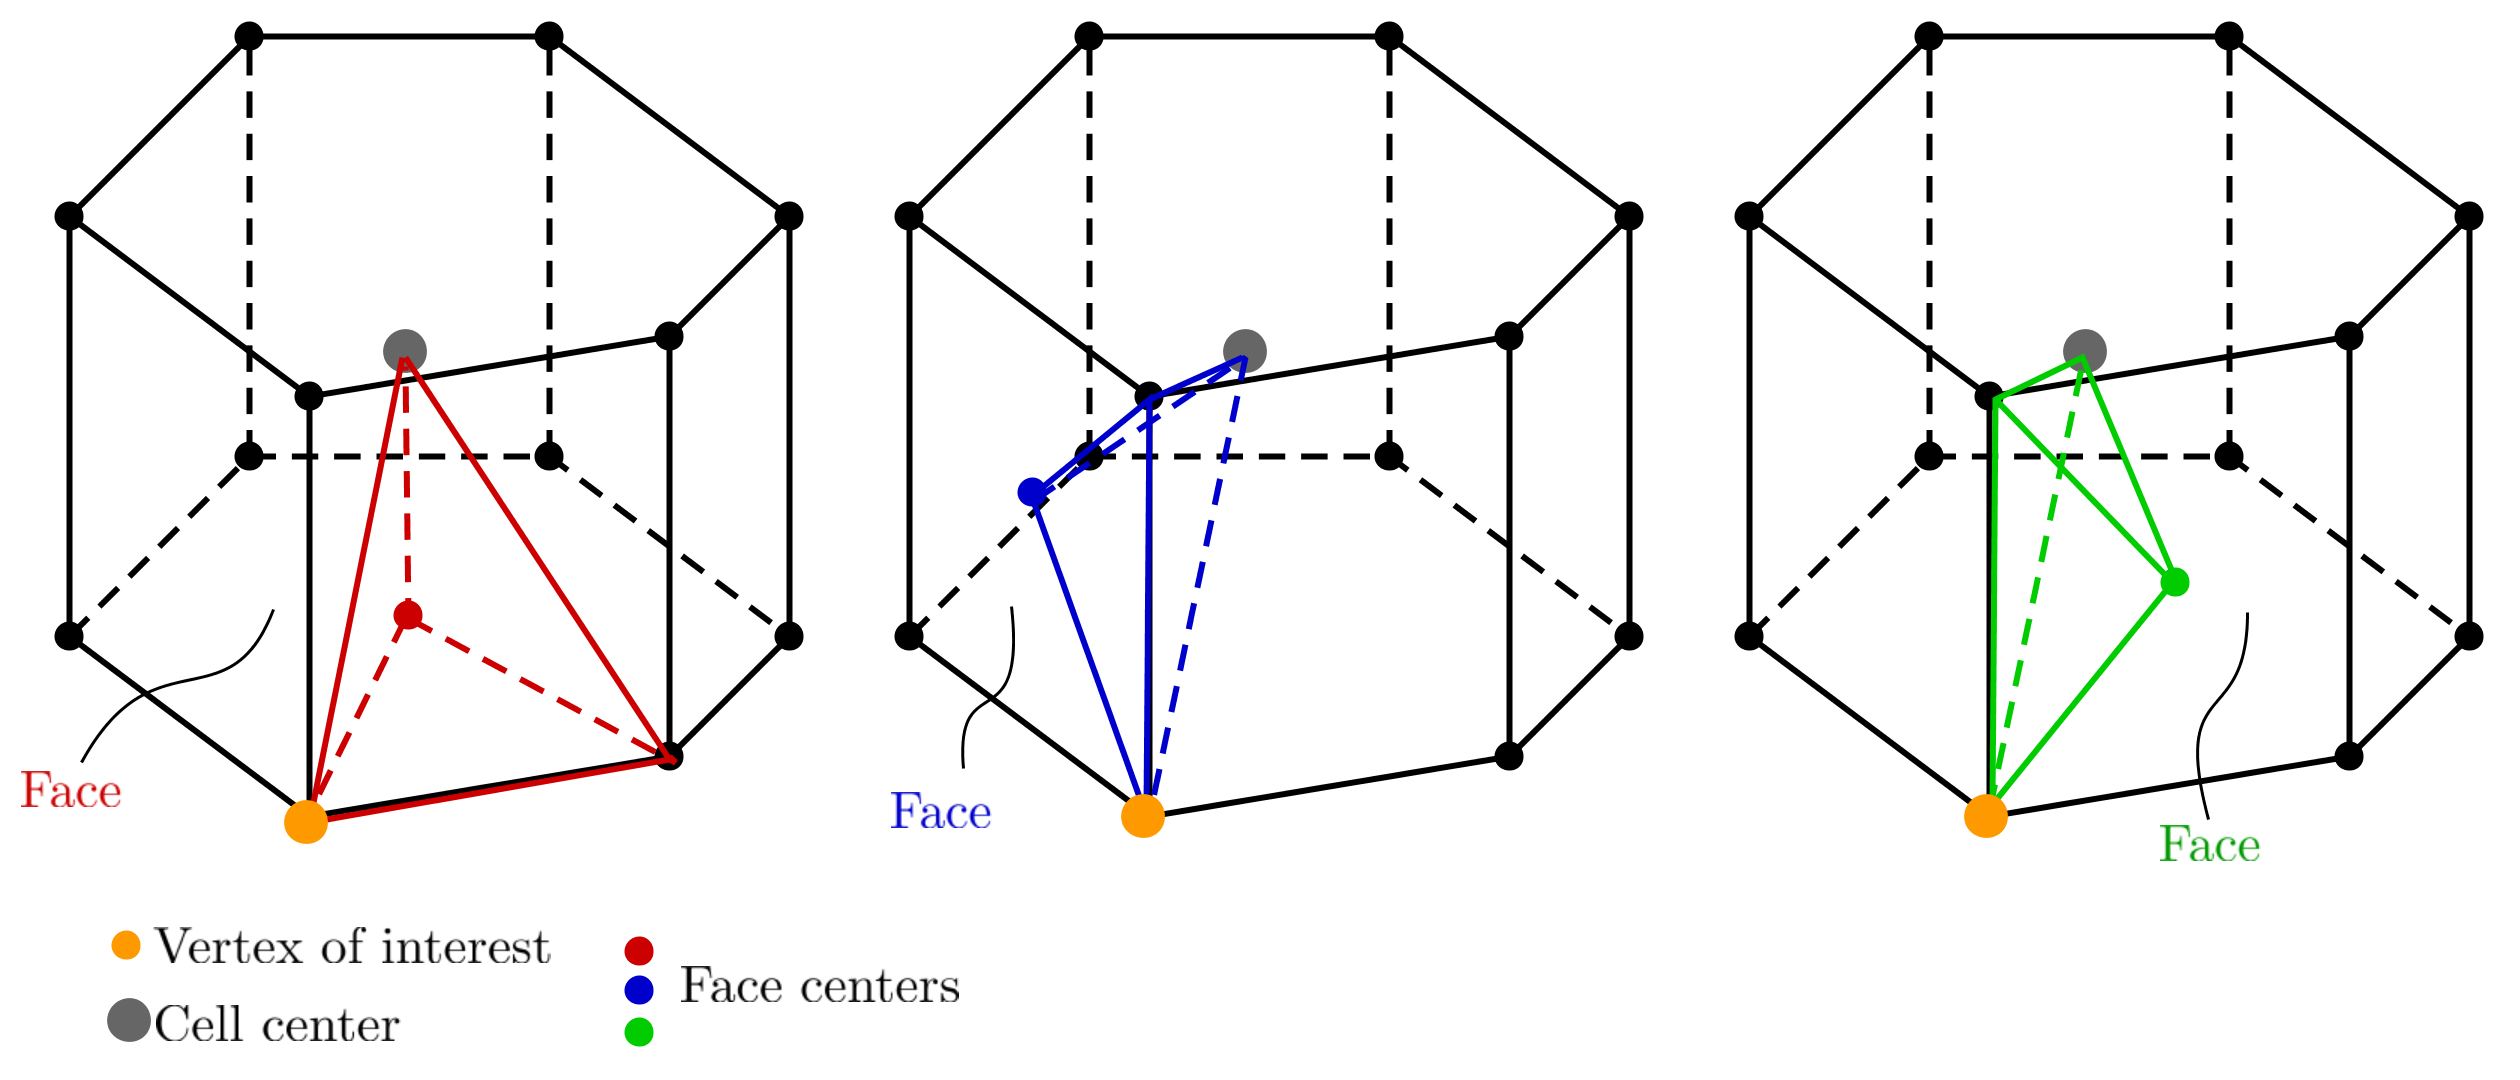
\includegraphics[width=1\linewidth]{LatexDraw/ThreeDTetrahedral}
\caption{Connection of the vertex of interest to the tetrahedrons that comprise the cell.}
\label{fig:threedtetrahedral}
\end{figure}

Firstly we split the polyhedron into faces, where each face can be a polygonal face. Each face is then split into a number of sides. A side is a tetrahedron, corresponding to a face, which is formed from each edge of the polygonal face where the vertex collection are the two vertices of the edge, the face center and the cell center. In other words the face center and the two vertices of the edge forms a triangle, and the cell center makes it a tetrahedron.
\newline 
\newline
As was the case with the polygon, all the other vertices $j$ (not $i$) are connected to the vertex of interest $i$ through the cell center. Again, we don't include the cell center as a point in the simulation so we have to spread its effect through to each of the vertices using the $\alpha_c$ factor. We also have face centered shape functions associated with the division of each polygonal face into sides. On each face, to which vertex $i$ belongs, the shape functions defined on the face centers will protrude into the tetrahedron under consideration (i.e. the tetrahedron associated with vertex $i$ associated with face $f$, side $s$). Therefore more clearly we can express the shape functions on a tetrahedron-by-tetrahedron basis

\beqn
P_i^{tet}(x,y,z) = 
\begin{cases}
\alpha_c N_c (x,y,z)    \quad \quad &\text{ no matter which tetrahedron} \\
+\beta_f N_f(x,y,z)  \quad \quad &\text{ if vertex }i \text{ is part of the face} \\
+N_i (x,y,z) \quad \quad &\text{ if vertex }i \text{ is part of the face-side pair} \\
\end{cases}
\eeqn
\newline
Figure \ref{fig:threedtetrahedralshape} shows the influence of a shape function (centered on a specific point as denoted by the start of an arrow) from a specific vertex (color). The orange colored vertex's influence is shown on the left most figure where the shape function is then the full equation because all of the conditions are met; i.e. $\alpha_c N_c$ is always present, vertex $i$ is indeed part of the face where this tetrahedron is defined and therefore $\beta_f N_f$ is present, finally it is also part of the side of the tetrahedron and therefore its basic shape function $N_i$ is present.
\newline
\newline
The middle figure shows the red vertex as a vertex that only has the contribution of $\alpha_c N_c$ and $\beta_f N_f$ because the red vertex is not on the side comprosing the tetrahedron of interest. The rightmost figure shows only the contribution of $\alpha_c N_c$ because the blue vertex is not part of any adjacent face. 

\begin{figure}[H]
\centering
\includegraphics[width=1\linewidth]{LatexDraw/ThreeDTetrahedralShape}
\caption{Influence of different vertices on the shape functions of within a tetrahedral portion of the cell.}
\label{fig:threedtetrahedralshape}
\end{figure}

\vspace{0.5cm}
\begin{algorithm}[H]
\ForEach{cell}{
$A^{N_v\stimes N_v}$ $\longleftarrow$ Initialize matrix \;
$b^{N_v\stimes 1}$ $\longleftarrow$ Initialize right hand side \;
\ForEach{vertex $i$}{
\ForEach{vertex $j$}{
\ForEach{face f}{
\ForEach{sub-tetrahedral s}{
\ForEach{quadrature point qp}{
$a_{ij}=a_{ij} + $ $\longleftarrow$ Eq. with $\tau_i$ and $b_j$ integrated over sub-triangle\;
$b_i = b_i +$ $\longleftarrow$ Eq. with $\tau_i$ and $b_j$ integrated over sub-triangle\;
}
}
}
}
}
$\phi$ $\longleftarrow$ Solve system\;
}
\caption{Polyhedron Based algorithm\label{algo:polyhedron}}
\end{algorithm}






\newpage
\chead{Code design}
\section{Code design}
\subsection{Overall strategy}
The neutron transport equation, with the scattering term and angular flux expanded, results in a large amount of variables to be stored and computed. Before introducing any form of spatial discretization the code has to handle the scalar flux moments $\phi_0 ... \phi_L$ for which we have a set for each group. When a spatial discretization scheme, along with a collection of cells, is introduced the problem size is scaled by the product of the number of cells and each cells respective degrees of freedom (DOF). Therefore the primary strategy of the code design is to support domain decomposition.

\subsection{Handling the mesh}
All mesh related items will be contained within the \xmloption{namespace} called \xmltag{chi\_mesh}. The primary item will be a storage space that will allow us to store all mesh entities into a global container we call the \xmltag{chi\_mesh::MeshHandler} class. All mesh creation and manipulations happen with a mesh handler, set to``current", and therefore in theory the code supports the use of multiple meshes, but that is a design feature to explore later.
\newline
\newline
Mesh construction, in general, can be split into 3 different methods:
\begin{itemize}
\item Use of pre-generated meshes (PGM). Such meshes have been built outside of the code and is in a form conducive to the direct construction of internal mesh data structures. This is a rather complex method since it requires knowledge of the source of such methods.
\item Generation of meshes within the code, i.e. internally generated meshes (IGM). Such a method will require the complete specification of the geometry within the code input structure as well as the algorithms required to create fully functional meshes with boundary identification.
\item Partial internally generated meshing (PIGM) . This method mostly implies the extrusion of a 2D surfaces to a 3D mesh but could extend to a 3D-printed type mesh..
\end{itemize}


\subsubsection{Pre-generated meshes}
Pre-generated meshes (PGMs) is a large topic for computational physics and not just a topic in this work. Many well developed packages exist that can produce high quality 3D meshes very efficiently and in most cases in parallel. Historically a software package generates a mesh file that is to be read by the code that uses it and for most applications a single file with all the mesh information suffices. However, in consideration of scaling simulations (i.t.o. number of spatial unknowns) one has to consider the ``friendliness" of such meshes towards scaling. 

\newpage
In the simplest case consider a mesh comprising hexahedrals, each cell will at minimum require:

\begin{itemize}[noitemsep]
\item \xmltag{4byte} The cell memory pointer.
\item \xmltag{byte} Number of vertices.
\item \xmltag{4byte} Pointer to vertex array.
\item \xmltag{8$\stimes$4bytes} Vertex index array.
\item \xmltag{byte} Number of faces.
\item \xmltag{4byte} Pointer to face inforation array.
\item \xmltag{4$\stimes$4 bytes} for each face to store vertex indices, \xmltag{96 bytes} total over the 6 faces.
\item \xmltag{4bytes} for each face storing the neighboring cell or boundary, \xmltag{16bytes} total over the 6 faces.
\item \xmltag{4bytes} The material index.
\end{itemize}

This is a total of 162 bytes for the storage of each cell and therefore we can fit approximately 6.6 million cells into 1 GB of memory. In practice though cell information includes a number of other variables that ease the lookup of information and the calculation of simulation inputs and in this regard it is more realistic to assume less than this number. However, if each process in a parallel simulation had to read and process the pregenerated mesh file then the total size of the mesh will essentially be capped by the average memory per core which is currently only as high as 3.5 GB per core (i.e. the Lawrence Livermore National Laboratory's Quartz cluster).
\newline
\newline
Scalable PGMs therefore require support for domain decomposition and methods to do so are being developed. The concept of generating cell counts in excess of 1 billion with a mesh generator is also a cause for concern since such a meshing tool will also require a means to do so efficiently and mostly in parallel as well. The end-specification however remains constant: PGMs need to exist in multiple files that are conducive to each process reading only the mesh that is allocated to it. Such efforts will require advanced domain decomposition and load balancing.
\newline
\newline
Support for PGMs has been an engineered features of ChiTech from the start because of the light-weight structure employed for containing mesh information. Interfaces can easily be developed to move meshes of any format into the database. To this end mesh information is stored within ChiTech as either \xmltag{CellPolygon} or \xmltag{CellPolyhedron}. The data structures for each of these is simple:
\vspace{0.5cm}
\begin{lstlisting}[language=c++]
class chi_mesh::Cell
{
public:
  int cell_global_id;
  int cell_local_id;
  std::pair<int,int> xy_partition_indices;
  std::tuple<int,int,int> xyz_partition_indices;
  int partition_id;
  Vertex centroid;
  int material_id;
 }
\end{lstlisting}
\newpage
\begin{lstlisting}[language=c++]
class chi_mesh::CellPolygon : public chi_mesh::Cell
{
public:
  std::vector<int>  v_indices;
  std::vector<int*> edges; ///< Stores arrays of edge indices
  std::vector<chi_mesh::Vector> edgenormals;
};
\end{lstlisting}
\vspace{0.25cm}
\begin{lstlisting}[language=c++]
class chi_mesh::CellPolyhedron : public chi_mesh::Cell
{
public:
  std::vector<int>       v_indices;
  std::vector<PolyFace*> faces;
};

struct chi_mesh::PolyFace
{
  std::vector<int> v_indices;
  std::vector<int*> edges;
  int face_indices[3];

  chi_mesh::Normal geometric_normal;
  chi_mesh::Vertex face_centroid;
};
\end{lstlisting}

In these data structures the normals and centroids can be computed as they are loaded and knowledge of neighbors is incorporated via \xmltag{edges} or \xmltag{face\_indices}. The base-class \xmltag{Cell} also doubles as a very lightweight ``ghost" cell which can conveniently be communicated between process to ease algorithm detail downstream of mesh loading. This is brings one to the topic of global cell indices which ChiTech uses. This eases the burden on engineering programmers where the concepts of graphs are not always solid. It also assists in restarting simulations with different partitioning strategies, sometimes even after a field function has already been computed. This strategy has proved very successful.
\newline
\newline
Reading decomposed 2D meshes will be incorporated in the \xmltag{VolumeMesherPredefined2D} volume mesher, and reading decomposed 3D meshes will be incorporated through the \xmltag{VolumeMesherPredefined3D} volume meshers.


\newpage 
\subsubsection{Internally generated meshes}
In the ideal case the code would have had the capability of generating, in parallel, a fully functional 3D mesh similar to what can be read with the predefined 3D mesh reader, however, a simple method of obtaining 3D meshes is to extrude 2D meshes and if the 2D meshes themselves are generated with the code then technically such a method is considered completely internally generated. The planning therefore is to use a Delaunay triangulation mesher to generate a 2D mesh and to extrude this mesh. The triangulation mesher will be named \xmltag{SurfaceMesherDelaunay} and the corresponding extruder will be named \xmltag{VolumeMesherExtruder}.

\subsubsection{Partially internally generated meshes}
As a subset of a 3D mesh generator using extrusion is the case where the 2D surface mesh is pre-defined and for this case we will name this process the \xmltag{SurfaceMesherPredefined} mesher which will feed into the \xmltag{VolumeMesherExtruder}.

\subsubsection{Meshing utilities}
In support of meshing operations a number of data structures and classes are defined to make the namespace all-inclusive. These are:
\begin{itemize}[noitemsep]
\item \xmltag{Vector}. Also doubling for \xmltag{Vertex}, \xmltag{Normal} and \xmltag{Node}. A general data structure that stores a vector of 3 components ($x,y,z$) and supports vector arithmetic, dot-products, cross-products and the L2-norm.
\item \xmltag{Edge} and \xmltag{EdgeLoop} for the storage of edges.
\item \xmltag{Face} and \xmltag{Polyface} for the storage of triangular and polygonal faces, respectively.
\item \xmltag{LineMesh} for storing a collection of lines used for the Delaunay mesher and to define boundaries.
\item \xmltag{SurfaceMesh} for storing either surface meshes read from file or store surface meshes generated within the code.
\item \xmltag{Boundary}, \xmltag{Region} and \xmltag{MeshContinuum} with each nesting from left to right is used to define continuum on which the mesh is defined.
\item \xmltag{CellTriangle}, \xmltag{CellPolygon} and \xmltag{CellPolyhedron} as a basic data structure to be handled by any process downstream. The end-goal of meshing is to have a collection of these.
\item \xmltag{Cellset} a collection of cell id's belonging to the local process.
\end{itemize}



\newpage 
\subsubsection{Mesh partitioning}
The current design for mesh partitioning requires unique global cell indices that map down to local cell indices. Cells are stored in a data structure named \xmltag{MeshContinuum} which gets pushed onto a \xmltag{Region} datastructure during the execution of the volume-mesher. This allows us to facilitate different regions of meshing. Within the \xmltag{MeshContinuum} the cells and their associated nodes are stored along with an important mapping vector \xmltag{local\_cell\_glob\_indices} which contains the global index mapping of local cells. Programmers can simply supply the local cell index to obtain the global cell index (the inverse mapping is also computed by the meshing routines).
\newline
\newline
Only local cells are fully defined, as either \xmltag{CellPolygon} or \xmltag{CellPolyhedron}, whereas non-local cells are stored as a near empty reference to the parent cell type \xmltag{Cell} which only stores its centroid and its partition id. We can call the parent cell type a ``ghost"-cell because it gets used as a placeholder when a cell is not local. Using these ghost cells is very advantageous for communicating data and is very easy to implement with an extruder mesher. An example of this is shown in Figure \ref{fig:cellmapping} below.


\begin{figure}[H]
\centering
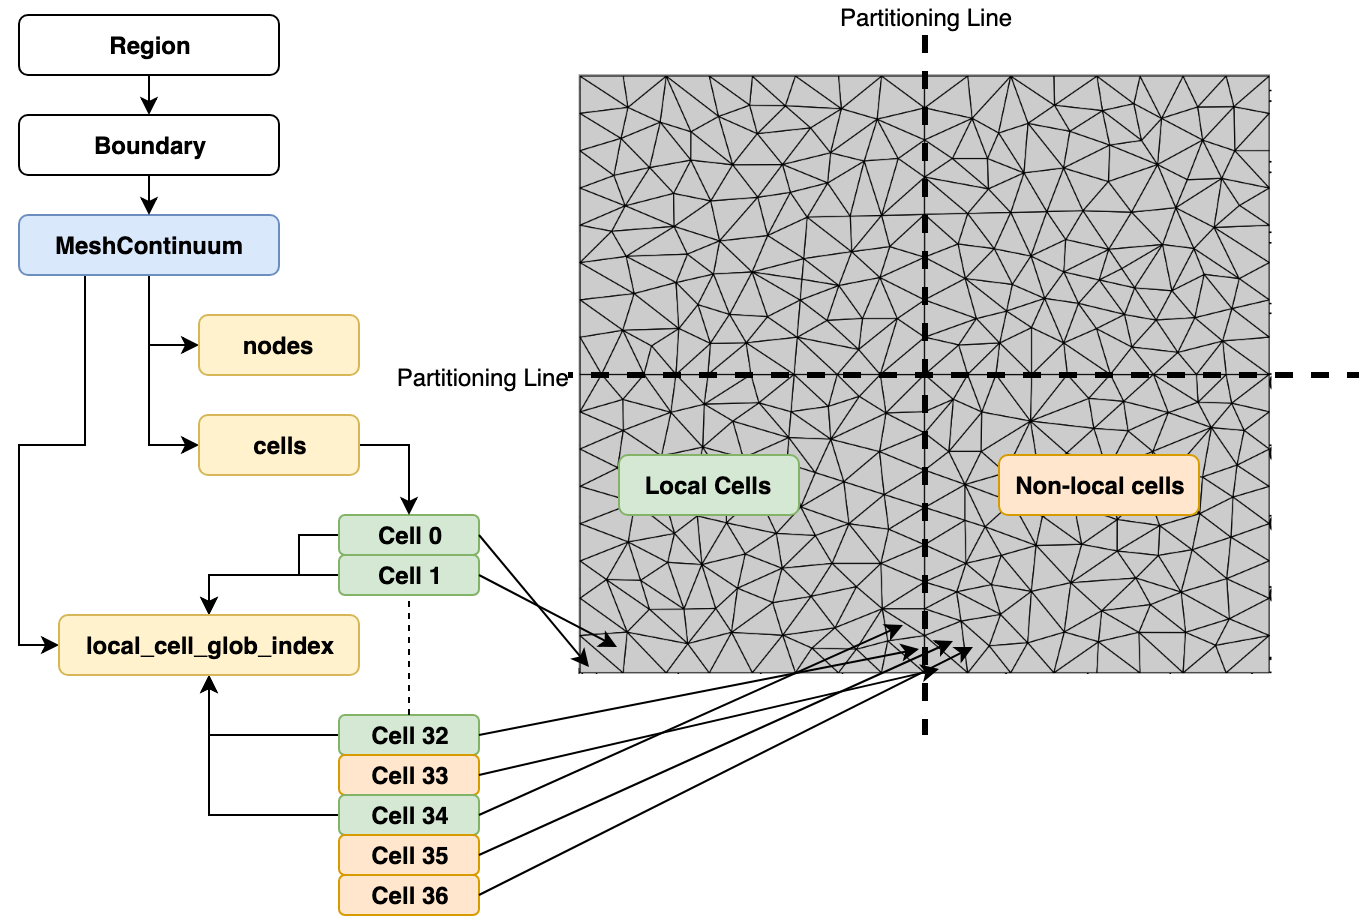
\includegraphics[width=0.9\linewidth]{LatexDraw/CellMapping}
\caption{Cell mapping logic.}
\label{fig:cellmapping}
\end{figure}



\vspace{1cm}
\subsection{Sweep Plane Data Structure (SPDS)}
When sweeping along a certain direction, cell dependencies are defined by the notion of upstream dependencies. That is, for current cell $i$ ... if the dot product of the sweep direction vector with the surface normal is negative (i.e. $\Omega \boldsymbol{\cdot} \hat{n} < 0$), and the face associated with that surface is connected to another cell $j$ and not a boundary, then cell $i$ is dependent on cell $j$. Connecting all the cells in this fashion for a particular direction results in the computer-science concept called a Directed-Graph, and a useful algorithm developed in this field is the \textbf{topological sort algorithm}. A topologically sorted Directed-Graph provides a sorted list of indices, which ensures that a seqeuntial reference to the cells pointed by these indices will reference cells with their dependencies already met during each subsequent downstream reference.
\newline
\newline
In spatial partitioning, where cells are allocated to parallel processes (we shall call these ``locations"), the cell dependencies can be either local or across a partitioning interface. To this end there can exist a local directed-graph as well as a global directed-graph, the latter meaning the dependency layout per-location.
For this project a topological sorting algorithm can certainly be developed, however, such algorithms have the restriction that the graph, to which the algorithm is to be applied, must be a Directed-Acyclic-Graph (DAG) which essentially means that cells cannot have cyclic dependencies. If cells, or locations, have a convex shape anywhere in space then cyclic dependencies will be introduced. This is an especially problematic topic for sweep codes and we will explore different ways in which to handle this topic.

\subsubsection{General notes on local and global cyclic dependencies}
There are two main strategies when dealing with cyclic dependencies.\newline

\textbf{Strategy A: Remove the cause}\newline
The first and simplest solution is to address the origin of the problem: convex shapes. If a convex shape causes a cyclic dependency, either on a local or global level, then one solution to this problem is to modify the problem geometry in such a way that the convex shapes are removed. Enforcing that local cells are convex is a fairly trivial solution to the local problem, however, for the global problem this essentially means that partitioning schemes need to ``cut" the problem mesh in order to ensure that partitioning interfaces between one location and another is always co-planar (or partitions are convex). This is a common strategy in transport codes.

\textbf{Pros:} There are no cyclic dependencies.\newline
\textbf{Cons:} Such a partitioning scheme is not common with other physics solvers (i.e. a hydrodynamic solver) and hence interfacing might be problematic. 
\newline
\newline
\textbf{Strategy B: ``Break" cycles}\newline
If a cyclic dependency is detected one can choose to preferentially assign one side of this dependency to a \textbf{delayed dependency}, where the information is obtained from a previous sweep (or zero on the first sweep). In order to solve the downstream information correctly this will then require iterations to converge the iterative nature of this scheme.

\textbf{Pros:} Cyclic dependencies are allowed and therefore enable the usage of domain decomposition similar to that used by hydrodynamic solvers.\newline
\textbf{Cons:} Cyclic iterations are introduced in addition to the normal numerical iterations which can have a large performance impact.

\subsubsection{Cyclic dependencies in this project}
By ensuring non-concave cells as well as non-concave partitions during mesh generation, strategy A is automatically supported. Strategy B requires more data structures but is implemented in $\chi$-tech as will be explained below.

\subsubsection{More detail on the Sweep Plane Data Structure}
Sweeping on meshes is handled by the \xmltag{sweep\_management} namespace, a subspace of the \xmltag{chi\_mesh} namespace. The first objective here is to initialize a \textbf{Sweep Place Data Structure} (SPDS) for each group of angles that will have the same sweep ordering therefore when given a grid and a direction ($\Omega$), the function call \xmltag{sweep\_management::CreateSweepOrdering} will firstly assemble a DAG of the local cells and create a single \textbf{Sweep Plane Local Subgrid }(\xmltag{SPLS}) that contains the indices of all the local cells, sorted topologically against the direction. This provides the ``fine-view" of sweep ordering and is stored in the vector \xmltag{SPLS::item\_id} on each SPDS. 
\newline
\newline
Cyclic dependencies complicates this process significantly. It is impossible to provide the complete scope here so the reader should take into consideration that only a portion of local cyclic dependencies are handled here.  The connection of the local DG for each SPDS is done in the function \xmltag{sweep\_management::} \xmltag{PopulateCellRelationships} and involves a loop over the local cells and populates 4 sets (\xmltag{std::set}). The first two are on a local cell-by-cell basis, the cell's predecessors and successors, in an absolute sense (whether there are cycles or not). The second two is on a location level, the location's predecessors and successors. The first two have temporary scope in the function \xmltag{CreateSweepOrdering} and are therefore passed by reference to this function. The second two are important items for the \xmltag{SPDS} and are populated directly on the SPDS structure. 

\begin{lstlisting}[language=c++]
void chi_mesh::sweep_management::PopulateCellRelationships(
         chi_mesh::MeshContinuum *grid,
         chi_mesh::sweep_management::SPDS* sweep_order,
         std::vector<std::set<int>>& cell_dependencies,
         std::vector<std::set<int>>& cell_successors)
\end{lstlisting}

\vspace{0.25in}
After \xmltag{PopulateCellRelationships} returns, a filter for Strongly Connected Components (SCC) is applied to the cell-by-cell successor- and predecessor-sets. SCCs are cells that have a successor that is also present in its predecessor set. If a SCC is found then the pair of components is registered in \xmltag{SPDS::local\_cyclic\_dependencies} and all other non-SCC components are added as graph edges in the DG. At this point of the algorithm we do not process the local cyclic dependencies further, it will be continued in the construction of the Flux Data Structures (FLUDS), however, since we did not add the graph edges corresponding to the SCCs we inherently removed the cyclic dependency and hence the local cycle is broken (hence the term ``breaking cycles"). With the DG in place we continue with the topological sorting and populating the \xmltag{SPLS}.
\newline
\newline
{\color{red} \textbf{Future feature:}} Note that at the time of writing, only a single sweep plane is assembled for the local sweep, however, future support for memory optimizing schemes are supported by allowing multiple sweep planes which in turn enable multi-threading within the same memory space. Such a scheme will introduce parallelism by dividing ``cells-in-play" between threads with each level representing a sweep plane.
\newline
\newline
Next we proceed with developing the ``course view" of the \xmltag{SPDS} which will generate one or more global sweep plane orderings from which the parallel nature arises, with each global sweep plane denoting the locations that are ``in-play". This process is also known as building the \textbf{Sweep Task Dependency Graph} (\xmltag{STDG}). The purpose of the ``course view" sweep planes is hard to explain without further context and will therefore be deferred to later. For now it will be stated that these planes are used in the Depth-Of-Graph sweep scheduling algorithm. 
\newline
\newline
Since the location predecessors- and successors-sets are available the algorithm continues by having each location broadcasting its complete dependency list. This allows each location to construct the global TDG which is required by the Depth-Of-Graph sweep scheduling algorithm. After the broadcast operation the dependency lists are filtered for Strongly Connected Partitions (SCP) by looping over each location $I$ and determining if the location itself has a dependence on location $J$, which in turn has a dependency on location $I$ (this happens linearly for location $I=0...N$). If a cyclic dependency is detected on location $I$ then the dependent location is removed from \xmltag{location\_dependencies} and added to \xmltag{delayed\_location\_dependencies}. Note that this process is not vice-versa, i.e. location $I$ will still remain on the successor list of location $J$. Subsequently the current location $I$ is added to the now delayed dependent location's \xmltag{delayed\_location\_successors} needed while populating the FLUDS. Note also that the now delayed dependent location $J$ does not remove the current location $I$ from either its dependency or successor list. In this way a TDG is constructed that is acyclic and we can proceed with a topological sorting.
\newline
\newline
After the topological sorting we arrange the ordering into work stages by determing the maximum rank of a location's dependencies and incrementing it by one. The first location in the ordering will have a rank of 0. The result of this algorithm can be seen in Figure \ref{fig:workstages} below. This sorting directly allows the application of the Depth-Of-Graph sweep scheduling algorithm since it assits in determining the depth of the graph for a given sweep ordering.

\begin{figure}[H]
\centering
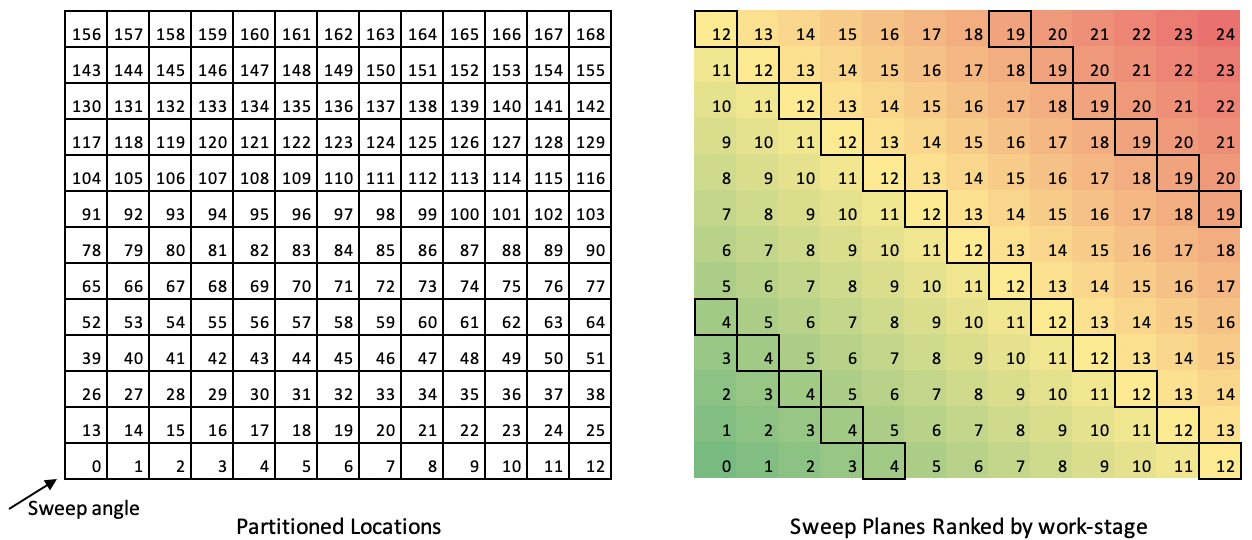
\includegraphics[width=0.9\linewidth]{Figures/WorkStages}
\caption{Depiction of arranging locations into sweep ordering ranked work stages.}
\label{fig:workstages}
\end{figure}


The Depth-Of-Graph sweep sceduling is described in \cite{ProvablyOptimalSweep} and involves sorting priorities according to how many locations are dependent on the current location's angleset (anglesets are described later) finishing a local sweep. It is dependent on all the locations and all the anglesets that are executed on the location. In general each location has to execute a local sweep for each angleset and for locations on the corner of the domain the angles orientated to the middle of the domain must have higher priority than the angles pointing out of the domain. More on this later.
\newline
\newline
Multiple sweep angles can share the same SPDS which is an aspect that needs to be managed by client code. For example: extruded meshes have the same sweep ordering for all polar angles in the top hemisphere given an azimuthal angle (same for the bottom hemisphere). The only inputs to the \xmltag{CreateSweepOrdering} is one of the angles that share this ordering, a reference to the grid, and whether cyclic dependencies are allowed. 
\newline
\newline
The final piece of each SPDS, and actually the most prominent, is the Flux Data Structure (\xmltag{FLUDS}) which is the topic of the next subsection but required to be mentioned here to give context to Figure \ref{fig:sweepordering} below, which depicts the hierarchy of datastructures.
\vspace{0.5cm}
\begin{figure}[H]
\centering
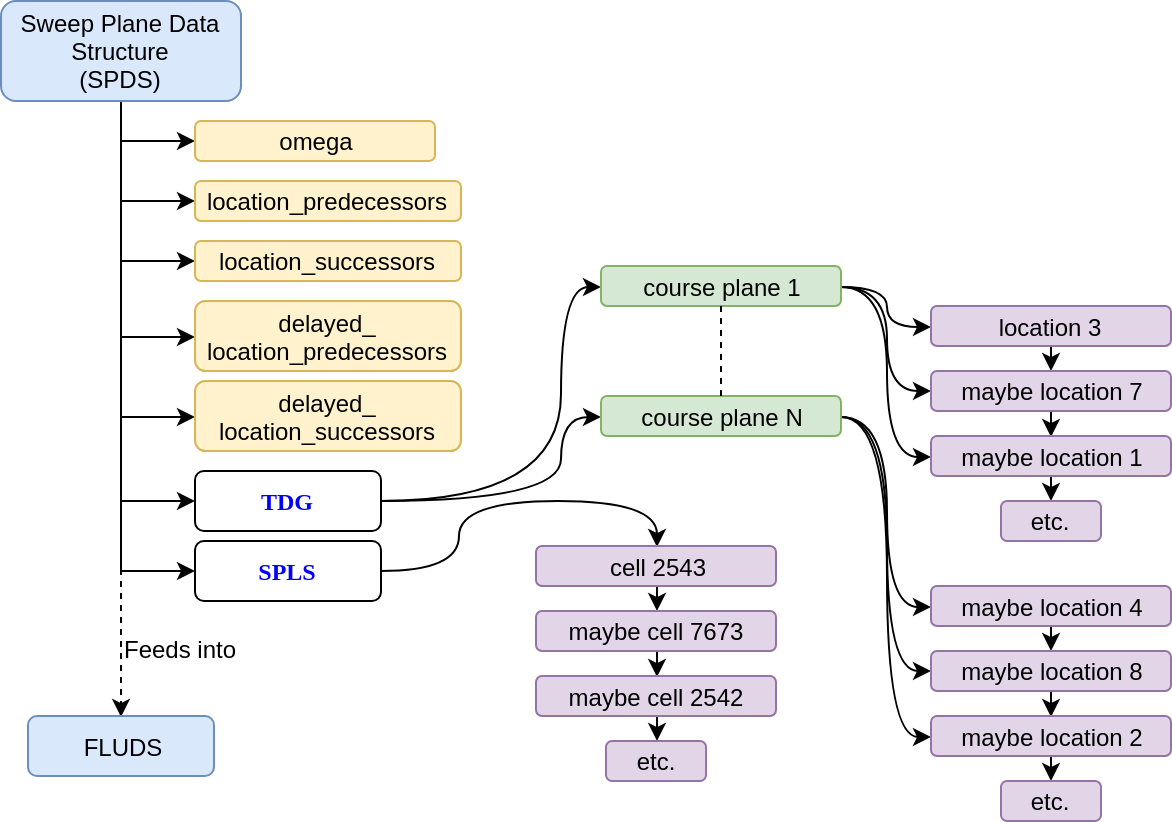
\includegraphics[width=0.9\linewidth]{LatexDraw/SweepOrdering}
\caption{Sweep ordering structure.}
\label{fig:sweepordering}
\end{figure}




\subsection{Flux Data Structure (FLUDS)}
A flux datastructure needs to cater for a host of requirements including the prevention of having to filter for stored information. PDT's STAPL library operates on the principle of filtering and plans are in progress \cite{AdamsSPDS} to develop a better implementation. Based on this work ChiTech has been equipped with a similar FLUDS.
\newline
\newline
Let us start with the local subgrid traversal (SPLS). A topological sorting of the Directed Graph was constructed during the development of the \xmltag{SPDS} datastructure and contains the order in which local cells are to be traversed in a sweep for a given angleset. One of the first memory saving principles is that a downstream cell can reuse the memory space where its incoming information was stored. We shall denote this concept as a ``lockbox" (\xmltag{vector<pair<int,short>> lockbox}) and to this end one can imagine an operator that places information in the next available slot and opens up a used slot whenever information is withdrawn. With this paradigm the maximum number of lock boxes is ultimately determined only by the maximum cells in play. It operates as shown in Figure \ref{fig:lockbox} below.

\begin{figure}[H]
\centering
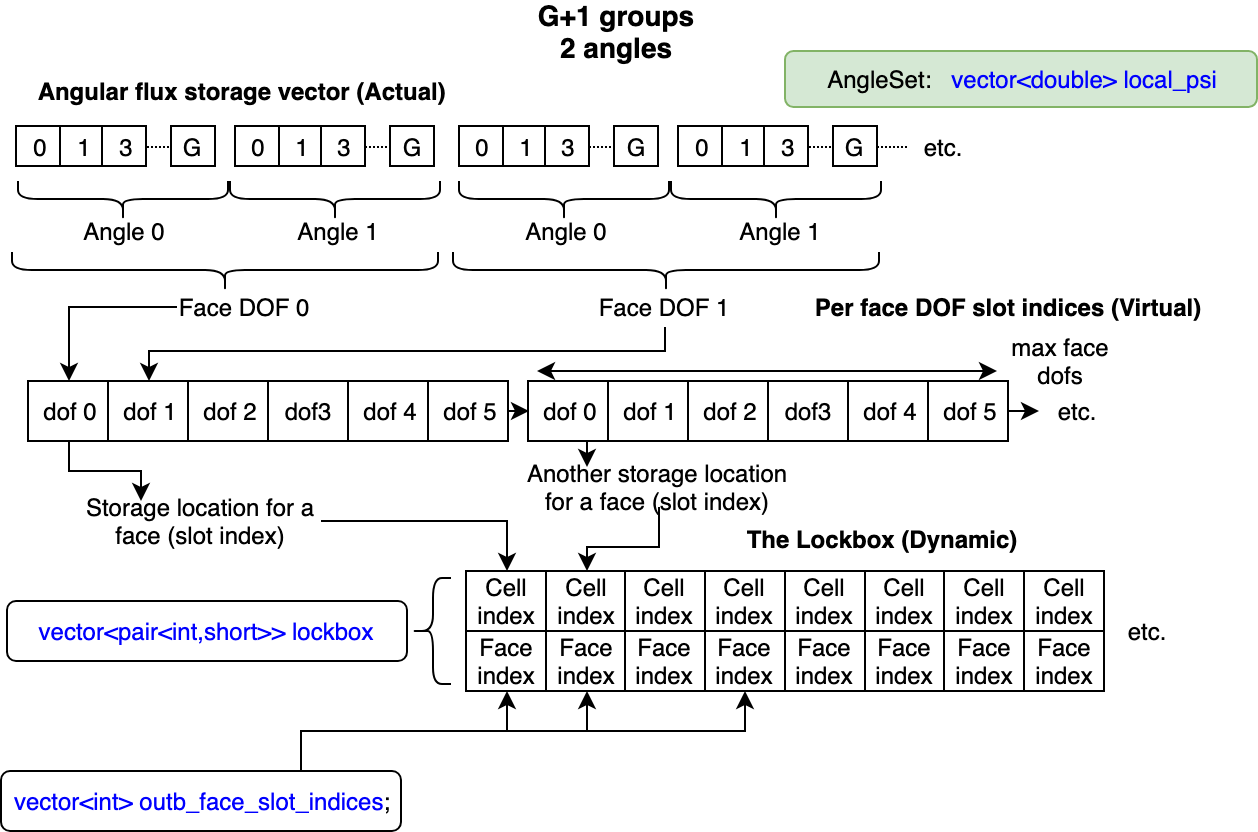
\includegraphics[width=0.9\linewidth]{LatexDraw/Lockbox}
\caption{Graphical depiction of the ``lockbox" concept.}
\label{fig:lockbox}
\end{figure}

Note in the figure above we only need to know the slot index of where a outgoing cell-face pair will store its data. The actual locations in the \xmltag{local\_psi} vector can be computed when the face DOF, angle, and group is provided.
\newline

Some discussion is also warranted on an idea developed in \cite{AdamsSPDS}. The idea is that, according to the above paradigm, the local $\Psi$ vector will be sized according to the maximum number of DOFs on any of the outgoing faces. This has the potential of allocating a large amount of unused memory if, for argument's sake, 95\% of the cells have the same amount of face dofs (say 4) and only 5\% have lets say 12 DOFs. Effectively 95\% of the faces will then allocate space for 12 DOFs per face where it only requires 4. The strategy to overcome this is now described.
\newline
\newline
A method is implemented on the grid class which will compute face statistics and avoid recomputing. The method  \xmltag{chi\_mesh::MeshContinuum::BuildFaceHistogramInfo} builds a face histogram but is never called directly. Rather the availibility of the histogram is assessed everytime a utility method is called. These utlility methods are:
\begin{itemize}
\item \xmltag{chi\_mesh::MeshContinuum::NumberOfFaceHistogramBins}. Returns the total number of bins in the histogram.
\item \xmltag{chi\_mesh::MeshContinuum::MapFaceHistogramBin}. Given an amount of face DOFs, returns the bin number into which the given number of face DOFs should be binned into.
\item \xmltag{chi\_mesh::MeshContinuum::GetFaceHistogramBinDOFSize}. Given a bin number, gives the upper bin boundary with regards to how many face DOFs are allowed in this bin.
\end{itemize}

\vspace{0.25in}
By default the face histogram is constructed as follows:
\begin{itemize}
\item A list of DOFs-per-face is constructed and sorted from smallest to largest. If there are F faces, there will be F list items. (i.e. 3,3,3,3,3, 4,4,4,4,4,4,4,4, 5,5,5,5,5,5)
\item The average and maximum DOFs per face is computed.
\item If the maximum-to-average ratio is $\le 1.2$ (can be customized) then all the faces are grouped into one bin designated to have a total number of face DOFs less than or equal to the maximum DOFs per face and the next step is skipped.
\item If the maximum-to-average ratio exceeds 1.2 then the following alogorithm is applied:
\begin{itemize}
\item A running averag, $n_{avg}$ is instantiated with initial value set to the smallest amount of DOFs per face. The current face size is also set to the smallest amount of DOFs per face ($f_{size}$).
\item The sorted face list is traversed (for each face $f$)
\item If the ratio of the number of DOFs on face $f$ to the running average exceeds 1.1 (can be customized) then a new bin is created. The bin represents the faces with number of DOFs less than or equal to the number of DOFs currently stored in $f_{size}$ and greater than the associated size limit of the previous bin.
\item $f_{size}$ is reassigned to the value of face $f$
\item After all faces are traversed, a final bin is added which represents all faces with number of DOFs smaller or equal to the maximum number of DOFs per face and greater than the size associated with the previous bin (if it exists). This last step also covers the case where the maximum to average ration is less than 1.2.
\end{itemize}
\end{itemize}

\vspace{0.25in}
By using this face histogram we can categorize faces between lockboxes and save a considerable amount of memory at the cost of storing the associated bin for each face. This is secondary to the requirement of storing a flag for faces that needs to take part in delayed angular flux handling. A strategy we employed here is to store positive numbers if an outgoing or incoming face is not part of a cyclic dependency, where this number represents the approriate lockboc, and negative numbers if the delayed angular flux data lockbox needs to be used.

\subsubsection{Some definitions}
\begin{itemize}
\item \textbf{Face Category:} The face-size histogram bin a face belongs to. If negative denotes a delayed dependency category instead.
\item $\mathbf{NDOF_{fmax}:}$ The maximum number of DOFs per face possible in the current local subgrid. 
\item \textbf{Lockbox slot:} Given $NDOF_{fmax}$, a slot has enough space to store all the angular fluxes of a given face. The total slot size is $NDOF_{fmax}{\times}GN_{stride}$
\item \textbf{Lockbox subslot} A block of data inside a lockbox slot large enough to store $GN_{stride}$ amount of data values (the amount fo data per DOF).
\item $\mathbf{GN_{stride}:}$ Each DOF will store $G{\times}N$ amount of angular fluxes. $G$ is the number of aggregated groups for the FLUDS and $N$ is the number of aggregated angles for the FLUDS.
\end{itemize}


\subsubsection{FLUDS $\alpha$-pass Local Portion (Slot Dynamics) } 
\xmltag{FLUDS::InitializeAlphaElements(...)}:
\begin{lstlisting}[language=c++]
std::vector<LockBox> lock_boxes(num_face_categories); //cell,face index pairs
LockBox              delayed_lock_box;
\end{lstlisting}
This pass firstly deals with storing the locations of where cells are to write or read angular fluxes from the \xmltag{local\_psi} vectors fo which there is a vector for each lockbox. Let us first discuss the outgoing faces. Since cells will be locally ``swept" in linear order each outgoing face will be the $i$-th face in a linear sequence. As long as an outgoing face knows which slot in the lockbox its first DOF is to store data, and which face-category it belongs to, it will then store each subsequent DOF in a location that follows the same sequence of DOFs. In other words cell $c$ outgoing face $f$, DOF-$0$ will have a lockbox slot address $S$ in \xmltag{local\_psi}, DOF-$1$ will store its data at lockbox subslot-address $S +GN_{stride}$, and in general DOF-$d$ will store its data at lockbox subslot-address $S +d{\times}GN_{stride}$ where $d=0...D$ ($D$ the amount of DOFs for face $f$). Therefore each cell's outgoing face only needs to know where to store its first DOF (i.e. DOF-$0$), the addresses for the other DOFs are inferred. To this end this algorithm will populate \xmltag{so\_cell\_outb\_face\_slot\_indices} and \xmltag{so\_cell\_outb\_face\_face\_category}.

\begin{lstlisting}[language=c++]
// This is a vector [cell_sweep_order_index][outgoing_face_count]
// which holds the slot address in the local psi vector where the first
// face dof will store its data
vector<vector<int>> so_cell_outb_face_slot_indices;

// This is a vector [cell_sweep_order_index][outgoing_face_count]
// which holds the face categorization for the face. i.e. the local
// psi vector that hold faces of the same category.
std::vector<std::vector<int>> so_cell_outb_face_face_category;
\end{lstlisting}

Consider now a downstream cell $c^*$ with incoming face $f^*$ with $f^*$ essentially being the same as face $f$ but with a different DOF order following the right hand rule. DOF-$0$ of face $f^*$ is NOT guaranteed to correspond to DOF-$0$ of face $f$ and therefore we need to determine the lockbox subslot address where each DOF will read its data. Fortunately, if we know the slot address for face $f$ we merely need to know the mapping of face $f^*$ DOF-$d$ to infer its subslot address. To this end the algorithm will populate \xmltag{so\_cell\_inco\_face\_dof\_indices} and \xmltag{so\_cell\_inco\_face\_face\_category}.
 
\begin{lstlisting}[language=c++]
// This is a vector [cell_sweep_order_index][incoming_face_count]
// that will hold a pair. Pair-first holds the slot address where this
// face's upwind data is stored. Pair-second is a mapping of
// each of this face's dofs to the upwinded face's dofs
vector<vector<pair<int,vector<int>> >> so_cell_inco_face_dof_indices;

// This is a vector [cell_sweep_order_index][incoming_face_count]
// which holds the face categorization for the face. i.e. the local
// psi vector that hold faces of the same category.
std::vector<std::vector<int>> so_cell_inco_face_face_category;
\end{lstlisting}

Even though this pass deals almost entirely with local data it serves as a good place to gather some information for dependent locations. The short name for dependent locations is \xmltag{deplocI} with the $I$ denoting the $i$-th location. Each FLUDS has a contiguous array for each dependent location which stores outbound angular fluxes in \xmltag{deplocI\_outgoing\_psi}, a vector of arrays (one per dependent location). Since these arrays are contiguous, in contrast to the ``slot" nature of the local outgoing angular fluxes, the arrays are subject to mapping. The first item to assist with this is a running counter per location of the amount of face dofs stored in it (\xmltag{deplocI\_face\_dof\_count}) which will also allow us to determine where a face's information is located in the $\Psi$-array (while building the count). 
\newline
\newline
Of course we also need to consider the dependent location will not have access to the local cells and faces and therefore we need to send some information to the location which can be used to map locations in the $\Psi$-array \textbf{relative to the dependent location} (remember that the face dof order will be different on the dependent location). To this end we have, at the lowest level, a \xmltag{CompactFaceView} storing where the face's data starts and also the global id's of the vertices
\vspace{0.25cm}
\begin{lstlisting}[language=c++]
//face_slot index, vertex ids
typedef std::pair<int,std::vector<int>> CompactFaceView;
\end{lstlisting}
This information gets pushed into a \xmltag{CompactCellView} and completes the ``packet" that the dependent location can use to map angular fluxes.
\vspace{0.25cm}
\begin{lstlisting}[language=c++]
//cell_global_id, faces
typedef std::pair<int,std::vector<CompactFaceView>> CompactCellView;
\end{lstlisting} 
We initialize these data structures at the beginning of the algorithm as

\vspace{0.25cm}
\begin{lstlisting}[language=c++]
//================================================== Initialize dependent
//                                                   locations
int num_of_deplocs = spds->location_successors.size();
deplocI_face_dof_count.resize(num_of_deplocs,0);
deplocI_cell_views.resize(num_of_deplocs,std::vector<CompactCellView>());
\end{lstlisting}

\newpage
\textbf{Filling the lockbox phase}:\newline
\xmltag{FLUDS::SlotDynamics(...)}:\newline
In this phase we loop over cells (in the sweep order) with an inner loop over faces. Note that during this phase we also determine the maximum degrees of freedom per face which will define our local storage requirement.
\newline
\newline
Initially the lockbox (vector of pairs) is empty, the first cell is encountered. 
\begin{itemize}
\item For each face of the cell it is determined if the face is incoming. Only if the incoming face has a local upstream cell or a boundary will this portion do anything, however, since this is the first cell in the sweep order it is guaranteed to not have a local upstream dependence. Subsequent cells will do more in this portion (described later).
\item We instantiate a vector of integers denoting slot indices.\newline
 (\xmltag{vector<int> outb\_face\_slot\_indices})
\item For each face of the cell (which will never be a large number hence the use of \xmltag{short}) it is determined if the face is outgoing (dot product with the sweep ordering's reference direction vector). 
\begin{itemize}
\item If it is outgoing and a local cell is downstream, we push the cell's global index and the associated face index \textbf{as a pair} to the lockbox. We also increment the outbound face counter and assign a new slot index.
\item If it is outgoing and a non-local cell is downstream, we first determine \xmltag{deplocI} (the $I$-th dependent location) mapped from \xmltag{SPDS::location\_successors}. The address where this face will store its angular fluxes in \xmltag{deplocI\_outgoing\_psi} is given by the  \xmltag{deplocI\_face\_dof\_count} counter. Once we have the address we can increment the counter which will subsequently contain the address for the next face. We can now push this information to the non-local slot ``address-book" named \xmltag{nonlocal\_outb\_face\_deplocI\_slot}.
\item We push the outbound face slot indices to the master data vector
\begin{lstlisting}[language=c++]
so_cell_outb_face_slot_indices.push_back(outb_face_slot_indices);
\end{lstlisting}
\end{itemize}


\end{itemize}

For each subsequent cell in the topological sorting we do the following:


\begin{itemize}
\item We first loop over all the incoming faces. From our meshing datastructure we will know the upstream neighbor of that face and because the neighbor is local we can determine (from the vertices) which face of the neighbor is associated with the current face. This provides us with a lookup pair (global cell index and face index). We then filter the lockbox with this pair as lookup and once we find the lockbox slot we empty it by assigning a negative number to the cell index. This denotes that the slot is open for a ``write" operation.
\item We again instantiate a vector of integers denoting slot indices.\newline
 (\xmltag{vector<int> outb\_face\_slot\_indices})
\item We now loop over the outgoing faces and repeat the same process as for the first cell. 
\end{itemize}

\bigskip
\bigskip

\textbf{Mapping local incident faces phase}:\newline
\texttt{FLUDS::IncidentMapping(...)}:\newline
With the lockbox slotting strategy developed we now start another phase. During the first phase we determined where outgoing faces will store their information. We now need to determine where each incident face DOF will read its data from.
\newline
\newline
The first level of this structure is a vector incremented by a incident face counter and then holding a pair comprising a lockbox slot and a vector. It is trivial to envision that we can determine an incident face's lockbox slot from the previously developed information, i.e. we know the neighboring cell's index and we can determine the associated face, therefore we can determine where that face will start storing its data (which will be a small contiguous block). We then just have to map each of the current cell's face DOFs to a location in this small contiguous block.

\begin{itemize}
\item For each cell in the topological sort we loop over only the incident faces. \xmltag{incoming\_face\_count} is incremented. We determine the face's upstream cell as well as its associated face. This determines the slot index.
\item We then do a mapping of the face DOFs. A fairly trivial operation by which we loop over the current cell face DOFs and internally loop over the upstream cell's face DOFs. If a match is found the mapping is pushed to the vector portion of the mapping pair.
\item We finally push the incoming face DOF mapping to the master data vector
\begin{lstlisting}[language=c++]
so_cell_inco_face_dof_indices.push_back(inco_face_dof_mapping);
\end{lstlisting}
\end{itemize}

\textbf{$\alpha$-pass Summary:}\newline
At the end of this pass we will have three primary FLUDS data structures:
\begin{enumerate}
\item \xmltag{vector<vector<int>> so\_cell\_outb\_face\_slot\_indices} \newline 
Given a cell's sweep ordering index, then outbound face counter, this structure holds the location index of the start of the face's outbound storage information.
\item \xmltag{vector<vector<pair>> so\_cell\_inco\_face\_dof\_indices} \newline 
Given a cell's sweep ordering index, then inbound face counter, this structure holds a pair. The first item of the pair is where the upstream information block starts and the second is a mapping of the face's DOFs inside this block.
\item \xmltag{vector<pair<int,int>> nonlocal\_outb\_face\_deplocI\_slot} \newline 
Given a non-local outgoing face count this vector stores a pair. The first portion of the pair stores the \xmltag{deplocI} index and the second portion stores the address of that face in the vector \xmltag{deplocI\_outgoing\_psi[deplocI]}.
\end{enumerate}


These data structures completely define where a cell can store its outgoing angular flux (per face) and also where it can retrieve its local incoming angular flux (per face). Accessing these locations within a sweep chunk is achieved with the three functions calls:
\newline
\begin{lstlisting}[language=c++]
double*  chi_mesh::SweepManagement::FLUDS::
 OutgoingPsi(int cell_so_index, int outb_face_counter,
              int face_dof, int n)
{
  // Face category
  int fc = so_cell_outb_face_face_category[cell_so_index][outb_face_counter];

  if (fc >= 0)
  {
    size_t index =
      local_psi_Gn_block_strideG[fc]*n +
      so_cell_outb_face_slot_indices[cell_so_index][outb_face_counter]*
      local_psi_stride[fc]*G +
      face_dof*G;

    return &(ref_local_psi->operator[](fc))[index];
  }
  else
  {
    size_t index =
      delayed_local_psi_Gn_block_strideG*n +
      so_cell_outb_face_slot_indices[cell_so_index][outb_face_counter]*
      delayed_local_psi_stride*G +
      face_dof*G;

    return &ref_delayed_local_psi->operator[](index);
  }
}
\end{lstlisting}

\begin{lstlisting}[language=c++]
double*  chi_mesh::SweepManagement::FLUDS::
UpwindPsi(int cell_so_index, int inc_face_counter,
             int face_dof,int g, int n)
{
  // Face category
  int fc = so_cell_inco_face_face_category[cell_so_index][inc_face_counter];

  if (fc >= 0)
  {
    size_t index =
      local_psi_Gn_block_strideG[fc]*n +
      so_cell_inco_face_dof_indices[cell_so_index][inc_face_counter].first*
      local_psi_stride[fc]*G +
      so_cell_inco_face_dof_indices[cell_so_index][inc_face_counter].
        second[face_dof]*G + g;

    return &(ref_local_psi->operator[](fc))[index];
  }
  else
  {
    size_t index =
      delayed_local_psi_Gn_block_strideG*n +
      so_cell_inco_face_dof_indices[cell_so_index][inc_face_counter].first*
      delayed_local_psi_stride*G +
      so_cell_inco_face_dof_indices[cell_so_index][inc_face_counter].
        second[face_dof]*G + g;

    return &ref_delayed_local_psi->operator[](index);
  }
}
\end{lstlisting}

\begin{lstlisting}[language=c++]
double*  chi_mesh::SweepManagement::FLUDS::
NLOutgoingPsi(int outb_face_counter,
                int face_dof, int n)
{
  int depLocI = nonlocal_outb_face_deplocI_slot[outb_face_counter].first;
  int slot    = nonlocal_outb_face_deplocI_slot[outb_face_counter].second;
  int nonlocal_psi_Gn_blockstride = deplocI_face_dof_count[depLocI];

  int index =
    nonlocal_psi_Gn_blockstride*G*n +
    slot*G + face_dof*G;

  return &ref_deplocI_outgoing_psi->operator[](depLocI)[index];
}
\end{lstlisting}


\subsubsection{FLUDS $\beta$-pass}
\texttt{FLUDS::InitializeBetaElements(...)}:\newline
This pass deals with the sending and receiving of cell geometrical information on partition interfaces and for determining where non-local upwind angular fluxes are stored.
\newline
\newline
\textbf{Phase A: If global cycles exist}\newline
This is a two step phase. The first is for each location to send compact cell views of the cells at the partition interfaces to each dependent location but only if the dependent is part of its \xmltag{delayed\_location\_successors} list. This is a non-blocking send which sends a serialized version of the \xmltag{deplocI\_cell\_views}. The receive step is a blocking-receive where each location receives compact cell views from its \xmltag{delayed\_location\_dependencies} list.
\newline
\newline
At the conclusion of this phase each location should have their delayed dependencies' compact cell views contained in \xmltag{delayed\_prelocI\_cell\_views}

\vspace{0.25in}
\textbf{Phase B: TDG partition interfaces}\newline
This phase has a blocking receive step followed by a non-blocking send step and will not dead-lock because the logic follows the task dependency graph. During the receive step, each location receives compact cells from its \xmltag{location\_dependencies} and during the send step each location sends compact cell views to its \xmltag{location\_successors} list.
\newline
\newline
At the conclusion of this phase each location should have their regular dependencies' compact cell views contained in \xmltag{prelocI\_cell\_views}

\vspace{0.25in}
\textbf{Phase C: Non-local incidence mapping}\newline
\texttt{FLUDS::NLIncidentMapping(...)}:\newline
For each cell in the sweep ordering:
\begin{itemize}
\item We loop over the faces of the cell. If the face is incident:
\begin{itemize}
\item We check to see if the upstream cell is non-local and only then do we proceed.
\item The location of the upstream cell is mapped to \xmltag{prelocI}. If the location is part of the regular dependencies list then this number will be positive and if the the location is part of the delayed dependencies list it will be negative -1. We handle each case separately:
\item \textbf{Regular dependency:} 
\begin{itemize}
\item We find the upstream cell in \xmltag{prelocI\_cell\_views}.
\item We find the associated face on the upstream cell.
\item We then map this face's DOFs to the upstream face's DOFs.
\item Finally we push all this information into \xmltag{nonlocal\_inc\_face\_prelocI\_slot\_dof}
\begin{lstlisting}[language=c++]
// This is a vector [nonlocal_inc_face_counter] containing
// AlphaPairs. AlphaPair-first is the prelocI index and
// AlphaPair-second is a BetaPair. The BetaPair-first is the slot where
// the face storage begins and BetaPair-second is a dof mapping
vector<pair<int,pair<int,vector<int>>>>
                  nonlocal_inc_face_prelocI_slot_dof;
\end{lstlisting}
\item We also push an empty version of this information into \xmltag{delayed\_nonlocal\_inc\_face\_prelocI\_slot\_dof} which is done so that we can reuse the non-local outgoing face counters.
\end{itemize}
\item \textbf{Cyclic dependency:}
\begin{itemize}
\item We find the upstream cell in \xmltag{delayed\_prelocI\_cell\_views}.
\item We find the associated face on the upstream cell.
\item We then map this face's DOFs to the upstream face's DOFs.
\item Finally we push all this information into \xmltag{delayed\_nonlocal\_inc\_face\_prelocI\_slot\_dof}
\begin{lstlisting}[language=c++]
// This is a vector [nonlocal_inc_face_counter] containing
// AlphaPairs. AlphaPair-first is the prelocI index and
// AlphaPair-second is a BetaPair. The BetaPair-first is the slot where
// the face storage begins and BetaPair-second is a dof mapping
vector<pair<int,pair<int,vector<int>>>>
                  delayed_nonlocal_inc_face_prelocI_slot_dof;
\end{lstlisting}
\item We also push an empty version of this information into \xmltag{nonlocal\_inc\_face\_prelocI\_slot\_dof} \textbf{but with the predecessor index negative}. This allows us to discern whether a face at a certain non-local incident face count is connected to a regular non-local dependency or a delayed non-local dependency.
\end{itemize}

\end{itemize}
\end{itemize}

\vspace{0.25in}
\textbf{$\beta$-pass Summary:}\newline
At the end of this pass we will have two additional FLUDS data structures:

\begin{enumerate}
\item \xmltag{vector<pair<int,pair<int,vector<int>>>>
    nonlocal\_inc\_face\_prelocI\_slot\_dof} \newline
This is a vector indexed by a non-local incoming face counter where each element contains an ``$\alpha$-pair". The $\alpha$-pair-first is the \xmltag{prelocI} index for the face. If negative this points to delayed incoming information. The $\alpha$-pair-second is a ``$\beta$-pair". The $\beta$-pair-first is the address where the face storage begins (in \xmltag{prelocI\_outgoing\_psi}) and $\beta$-pair-second is a vector indexed by the current face's DOFs and maps the current face's DOFs to the upstream face's DOFs.

\item \xmltag{vector<pair<int,pair<int,vector<int>>>>
    delayed\_nonlocal\_inc\_face\_prelocI\_slot\_dof} \newline
This is a vector indexed by a non-local incoming face counter where each element contains an ``$\alpha$-pair". The $\alpha$-pair-first is the \xmltag{delayed\_prelocI} index for the face. The $\alpha$-pair-second is a ``$\beta$-pair". The $\beta$-pair-first is the address where the face storage begins (in \xmltag{delayed\_prelocI\_outgoing\_psi}) and $\beta$-pair-second is a vector indexed by the current face's DOFs and maps the current face's DOFs to the upstream face's DOFs.
\end{enumerate}

These data structures completely define where a face can retrieve is non-local incoming angular flux (per face). Accessing these locations within a sweep chunk is achieved with the following single function call:

\begin{lstlisting}[language=c++]
double*  chi_mesh::SweepManagement::FLUDS::
 NLUpwindPsi(int nonl_inc_face_counter, int face_dof,int g, int n)
{
  int prelocI =
    nonlocal_inc_face_prelocI_slot_dof[nonl_inc_face_counter].first;

  if (prelocI>=0)
  {
    int nonlocal_psi_Gn_blockstride = prelocI_face_dof_count[prelocI];
    int slot =
        nonlocal_inc_face_prelocI_slot_dof[nonl_inc_face_counter].second.first;

    int mapped_dof =
        nonlocal_inc_face_prelocI_slot_dof[nonl_inc_face_counter].
            second.second[face_dof];

    int index =
        nonlocal_psi_Gn_blockstride*G*n +
            slot*G +
            mapped_dof*G + g;

    return &ref_prelocI_outgoing_psi->operator[](prelocI)[index];
  }
  else
  {
    prelocI =
        delayed_nonlocal_inc_face_prelocI_slot_dof[nonl_inc_face_counter].first;

    int nonlocal_psi_Gn_blockstride = delayed_prelocI_face_dof_count[prelocI];
    int slot =
        delayed_nonlocal_inc_face_prelocI_slot_dof[nonl_inc_face_counter].second.first;

    int mapped_dof =
        delayed_nonlocal_inc_face_prelocI_slot_dof[nonl_inc_face_counter].
            second.second[face_dof];

    int index =
        nonlocal_psi_Gn_blockstride*G*n +
            slot*G +
            mapped_dof*G + g;

    return &ref_delayed_prelocI_outgoing_psi->operator[](prelocI)[index];
  }

}
\end{lstlisting}



\subsection{Groups and Angles}
As is often the case with neutral particle transport, the notion of a \xmltag{Group} arises mostly because the material properties are dependent on particle energy and hence require discretization in the energy domain. Particles can be transfered (i.e. scattered) back and forth between energy groups and hence we will require a material property called the \xmltag{ScatteringMatrix} which holds the likelihood of a particle scattering from group $g'$ to group $g$. Hence, for $G$ groups, the scattering matrix can be a $G\stimes G$ dense matrix, however in reality we can introduce some sparsity to these matrices since particles can scatter in a band of groups.\newline 

Because the problem size essentially scales with the number of groups, a very useful memory-saving technique is to split the collection of groups into a number of distinct collections, each called a \xmltag{Groupset} with unique properties. One important property that a groupset can have is it \xmltag{ProductQuadrature} rule for integration over angle space. Particular quadrature rules are discussed in the appendices. Discrete ordinate angles directly related to the abscissae used in the quadrature rule and therefore the \xmltag{Angles} are determined by these rules. As will be seen later, angles, like groups, can have similar properties which we can group into \xmltag{AngleSets} in order to speed up parallel computations.
\newline
\newline
An additional feature incorporated into groupsets is \xmltag{Groupset::Subsets} which allows further seperation of anglesets. This has proven advantageous for the development of ``feedstock" to the sweeping algorithm where the parallel efficiency is dominated by the ratio of idle tasks to total number of tasks.

\subsubsection{Groupset Hierarchy}
At the topmost level a groupset hierarchy is as shown in figure \ref{fig:groupsethierarchy}. The sweep infrastructure is primarily focused on the angle aggregation portion of the hierarchy.

\begin{figure}[H]
\centering
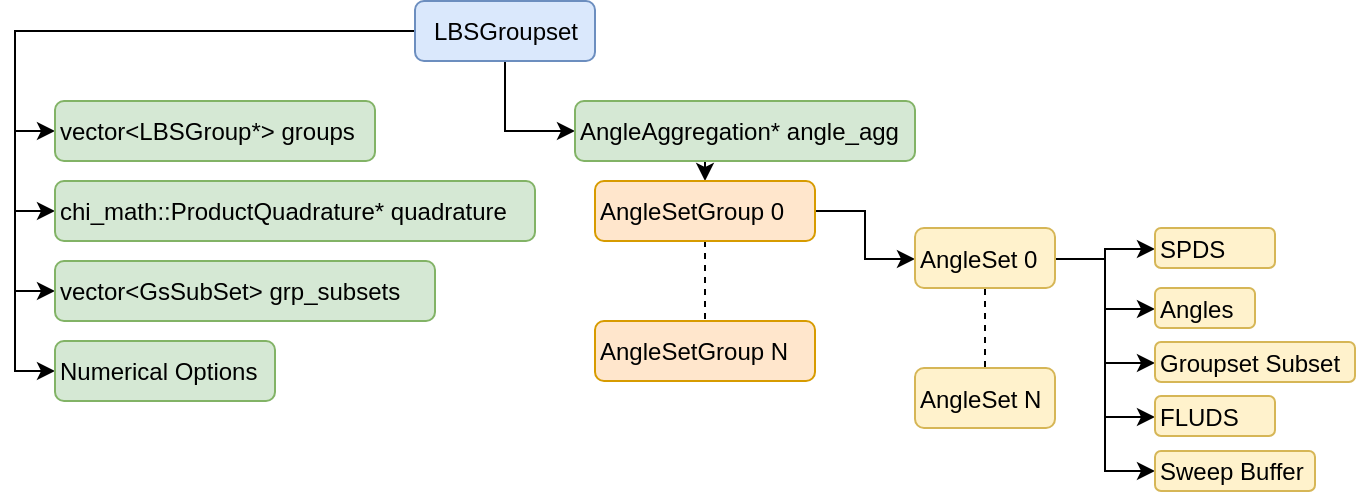
\includegraphics[width=0.9\linewidth]{LatexDraw/GroupsetHierarchy.png}
\caption{Groupset Hierarchy}
\label{fig:groupsethierarchy}
\end{figure}

\subsubsection{Angle Aggregation}
The primary interface to sweep routines is for client code to populate the \xmltag{AngleAggregation} data structure. This data structure comprises a number of \xmltag{AngleSetGroup} structures which in turn contains \xmltag{AngleSet} structures. The angle-set is the lowest level of structure and connects all the necessary elements for sweep chunks to be executed. It needs to be connected to a \xmltag{SPDS} such that all the angles that it holds have the same SPDS. For extruded meshes this often involves all or a number of polar angles sharing the same SPDS (this is called ``polar-angle aggregation"). For completely unstructured meshes an angle-set will most likely contain only a single angle (this is called ``single-angle aggregation"). An angle-set is not required to be associated with all the groups in a group-set and can be prescribed a subset of the group-set. Finally an angle-set is connected with a \xmltag{FLUDS} and an associated \xmltag{SweepBuffer}.


\vspace{0.25in}
\subsubsection{AngleSetGroup}
In general a sweep algorithm will have a sweep ordering where cells will be swept from positions where their dependencies are met. For a Rectangular Parallelipiped (RPP) domain this normally means that the cells located on the corners can be swept at the same time. In such cases it would be useful to arrange angle-sets by octant. In a more general sense there can be an arbitrary amount of ``groups" and this can be controlled by client code.

\begin{figure}[H]
\centering
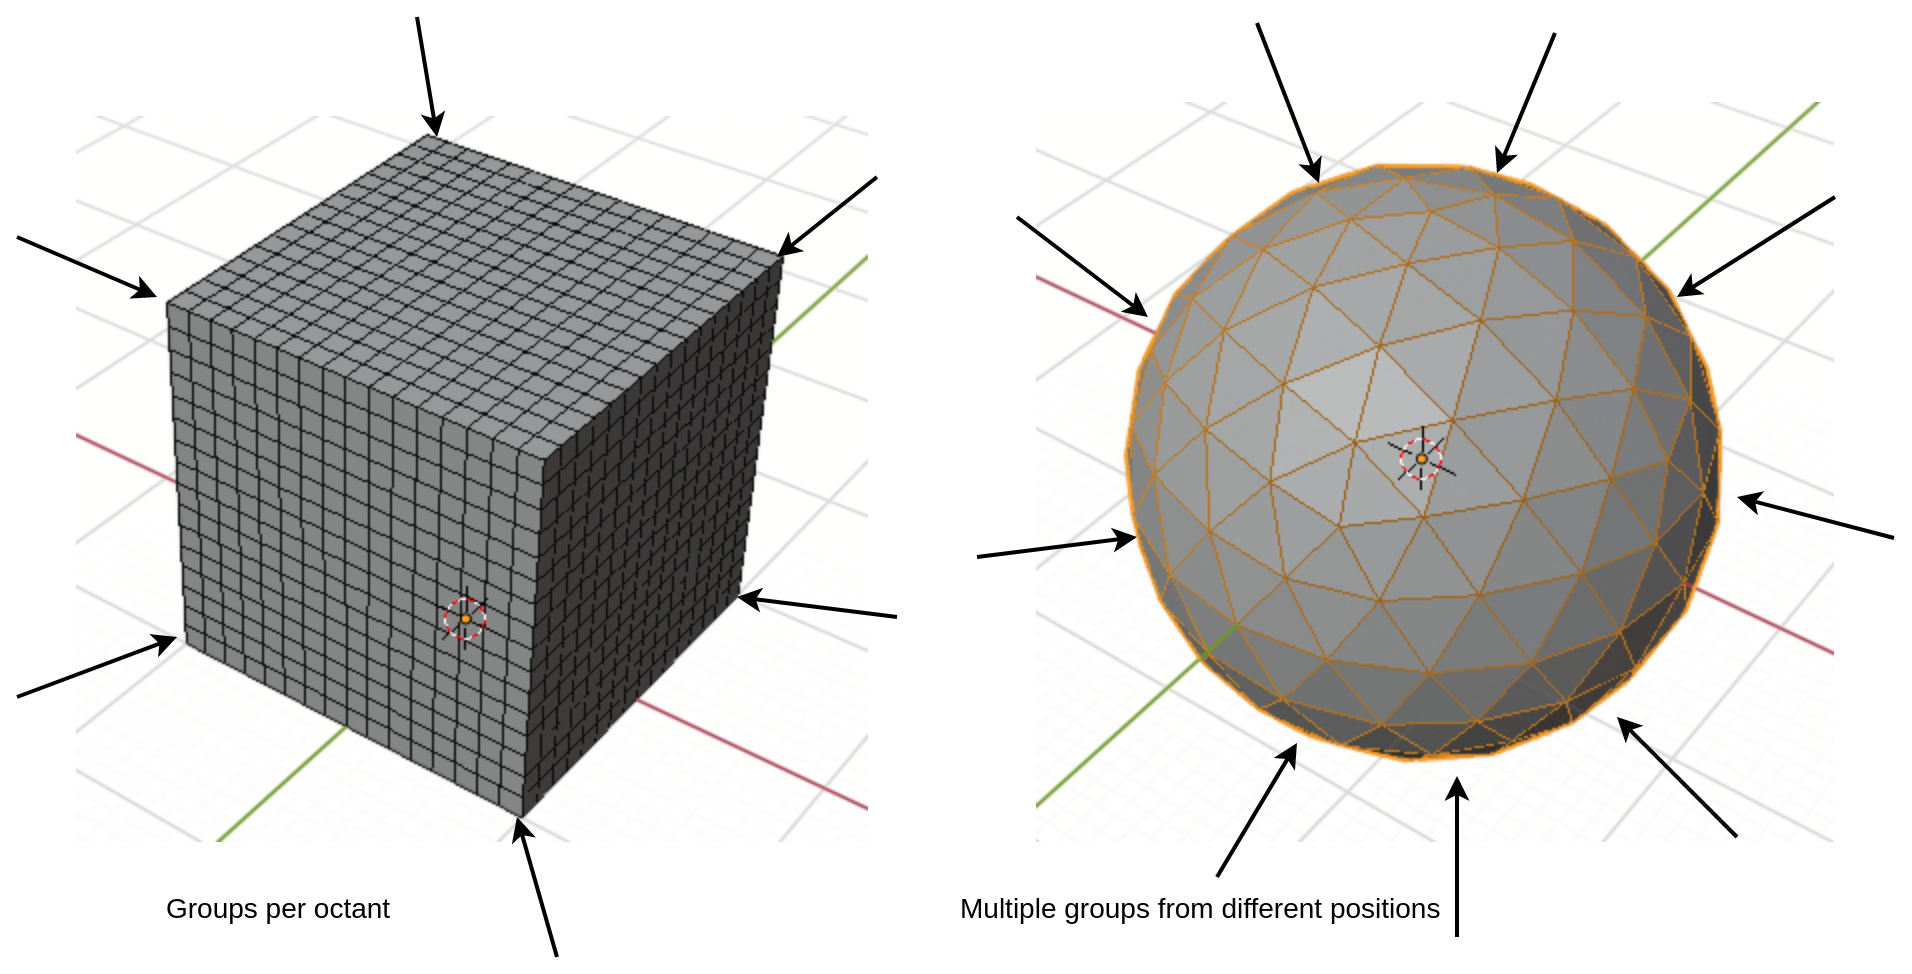
\includegraphics[width=1.0\linewidth]{LatexDraw/AngleSetGroups}
\caption{Angle set groups for different geometry types.}
\label{fig:anglesetgroups}
\end{figure}

\vspace{0.25in}
\subsubsection{AngleSet}
The angle-set is the fundamental piece of the sweep algorithm. It manages the angular fluxes and is the unit of logic most important to the flow of the algorithm. The most prominent data members are the following:

\begin{lstlisting}[language=c++]
int                     num_grps;
int                     ref_subset;
SPDS*                   spds;
vector<SweepBndry*>&    ref_boundaries;
FLUDS*                  fluds;
vector<int>             angles;
vector<vector<double>>  local_psi;
vector<double>          delayed_local_psi;
vector<vector<double>>  deplocI_outgoing_psi;
vector<vector<double>>  prelocI_outgoing_psi;
vector<vector<double>>  boundryI_incoming_psi;

vector<vector<double>>  delayed_prelocI_outgoing_psi;
vector<double>          delayed_prelocI_norm;

chi_mesh::SweepManagement::SweepBuffer sweep_buffer;
\end{lstlisting}


\subsubsection{Sweep Buffers}
A \xmltag{SweepBuffer} is an object that attaches to an angleset to manage information during a sweep. In a broad sense it fulfills three functions i) it decomposes contiguous blocks of angular flux data into messages that can more efficiently utilize a computers communication infrastructure, ii) it assigns blocks of memory at appropriate stages, iii) it de-allocates memory at appropriate stages of the sweep workflow. 
\newline
\newline
When an angleset is created the \xmltag{SweepBuffer::BuildMessageStructure} method is called from the constructor of the angleset. This method then determines the overall size of data to be sent and received from the FLUDS associated with the angleset. The are three sets of data to handle, successors, predecessors, and delayed predecessors. For each item in these sets the data is divided into messages all of whom needs to fit within the so-called ``Eager limit". The eager limit is an architecture dependent message size limit after which messages will undergo buffering. If messages are smaller than the eager limit the communication system can more efficiently and predictably send blocks of data as packets. Each message is outfitted with a \textbf{tag} which is a unique number to identify the message between a sender and a receiver.
\newline
\newline
\textbf{A note on tag numbers:}\newline
For a given interface between location $I$ and $J$, angular fluxes get passed using non-blocking MPI send-functions. These functions require the specification of the sender, the receiver, the message size, and the message tag. Upon receipt, messages do not uniquely identify on message size (i.e. messages can be truncated) and we are faced with an issue regarding the fact that multiple angle sets can match the unique sender-receiver combination. Unique messages therefore require unique tags for a given sender-receiver pair. In order to achieve this we have to understand that sender-receiver pairs can come in two variants, the first is the normal predecessor-succesor relationship, the second is the delayed predecessor-succesor relationship. As a reminder, the delayed relationship arises because of cyclic dependencies between partitions.
\newline 
\newline
A simple solution to this problem is to find the maximum message count, $mc_{max}$, across all locations and all anglesets, $n=0...N$ then construct a tag number as follows:

\beqn
n_{tag} = mc_{max} \times n \ + \ m
\eeqn

where $m$ is the message number for the given $IJ$ interface.
\newline
\newline
During an actual sweep each angleset has two allowable execution permissions encapsulated in a call to advance the angleset (\xmltag{AngleSet::AngleSetAdvance}):\newline \xmltag{ExecutionPermission::EXECUTE} which commands the angleset to execute if it is ready, and \newline \xmltag{ExecutionPermission::NO\_EXEC\_IF\_READY} which will inhibit the angleset from executing even if it is ready.
Whether or not an angleset is ready to execute is determined by whether it received all of its upstream dependencies (meaning all messages are received). Part of advancing is therefore to receive messages. With this paradigm the sweep scheduler can continuely loop over all the anglesets and advance them as far as they can, which in most cases mean to receive all the messages available. Only the scheduled angleset is given permission to execute and once it indicated that it executed the scheduler moves to the next scheduled angleset. 
\newline
\newline
The sweep buffer's second and third general functions are captured within a call to advance its angleset. If the angleset already executed it will check if the angleset is done sending downstream information. If it is not, a call to \xmltag{SweepBuffer::ClearDownstreamBuffers} will be made to clear the downstream buffers. If the angleset has not executed, a call to \xmltag{SweepBuffer::ReceiveUpstreamPsi} will be made. This method will allocate the receive buffer memory and attempt to receive the predeveloped message list. If a message was already received it will not try to receive it again and therefore can return one of two states:
\begin{itemize}
\item \xmltag{AngleSetStatus::RECEIVING}, indicating that none or only some of the upstream messages have been received.
\item \xmltag{AngleSetStatus::READY\_TO\_EXECUTE}, indicating that all messages were received.
\end{itemize}

If an angleset is ready to execute and it has been given permission to do so it will make a call to
\xmltag{SweepBuffer::InitializeLocalAndDownstreamBuffers} which is the big memory allocation for the local angular flux vectors as well as the vector to hold data for downstream locations. As can be seen from the logic here this memory allocation is deferred to the last possible moment in order to keep the overall program memory usage to a minimum. After the buffers have been initialized, the actual sweep chunk is executed.
\newline
\newline
After the sweep chunk executed communication to downstream locations are initiated with a call to \xmltag{SweepBuffer::SendDownstreamPsi} after which the local $\Psi$ and receive buffers will be cleared (since they are no longer needed) with a call to \xmltag{SweepBuffer::ClearLocalAndReceiveBuffers}. The send buffers are not cleared yet because an asynchronous send operation was used in \xmltag{SweepBuffer::SendDownstreamPsi} and is instead prepended to the advancement step.
\newline 
\begin{lstlisting}[language=c++]
chi_mesh::sweep_management::AngleSetStatus
chi_mesh::sweep_management::AngleSet::
AngleSetAdvance(chi_mesh::sweep_management::SweepChunk *sweep_chunk,
                int angle_set_num,
                chi_mesh::sweep_management::ExecutionPermission permission)
{
  typedef AngleSetStatus Status;

  if (executed)
  {
    if (!sweep_buffer.done_sending)
      sweep_buffer.ClearDownstreamBuffers();
    return AngleSetStatus::FINISHED;
  }

  Status status = sweep_buffer.ReceiveUpstreamPsi(angle_set_num);

  if      (status == Status::RECEIVING) return status;
  else if (status == Status::READY_TO_EXECUTE and
           permission == ExecutionPermission::EXECUTE)
  {
    sweep_buffer.InitializeBuffers();

    sweep_chunk->Sweep(this); //Execute chunk

    //Send outgoing psi and clear local and receive buffers
    sweep_buffer.SendDownstreamPsi(angle_set_num);
    sweep_buffer.ClearLocalAndReceiveBuffers();

    executed = true;
    return AngleSetStatus::FINISHED;
  }
  else
    return AngleSetStatus::READY_TO_EXECUTE;
}
\end{lstlisting}

Apart from the flow of the sweep system is the receipt of delayed angular data.


\newpage
\subsubsection{SweepScheduler}
The design of the \xmltag{SweepScheduler} system is inspired by the work done in \cite{ProvablyOptimalSweep}. At a fundamental level the TDG can be executed in a ``first-come-first-serve" basis. This basic scheduling cannot really be considered a ``scheduling algorithm" because each AngleSetGroup merely waits for its upstream dependencies to be met before executing. This was the first algorithm made available in the code (\xmltag{SchedulingAlgorithm::}\xmltag{FIRST\_IN\_FIRST\_OUT}) which we shall just refer to as the FIFO algorithm denoting ``first-in-first-out", and only scheduled tasks on AngleSetGroup-level (note: AngleSetGroup is equivalent to octanct in \cite{ProvablyOptimalSweep}). If an angleset in an angleset-group executed the scheduler first allows another angleset-group to advance before returning to the anglesetgroup that just advanced.

The FIFO algorithm does not prioritize anglesets in any fashion and therefore cannot be as optimal as an algorithm that does so.
\newline
\newline
The Depth-Of-Graph (DOG) algorithm is described succinctly in \cite{ProvablyOptimalSweep} and is implemented in the code with the denotation \xmltag{SchedulingAlgorithm::}\xmltag{DEPTH\_OF\_GRAPH}. In this algorithm an angleset on a given location can be characterized by its direction and the number of locations that are downstream. The latter characteristic is captured in the notion of Depth-Of-Graph and denotes the number of workstages downstream. Recall that the workstages structure has been developed during the intial creation of a SPDS data structure (see Figure \ref{fig:workstages}). For brevity we will denote the number of workstages downstream as $D$, the same denotation used \cite{ProvablyOptimalSweep}. Angleset priority is then developed by sorting the angleset according to the following rules:
\begin{itemize}
\item Tasks with larger $D$ have higher priority
\item If multiple anglesets have the same $D$ then anglesets with $\Omega_x>0$ have priority.
\item If multiple anglesets have the same $D$, and the same sign on $\Omega_x$, then tasks with $\Omega_y>0$ have priority
\item If multiple anglesets have the same $D$, and the same sign on $\Omega_x$ and $\Omega_z$, then tasks with $\Omega_z>0$ have priority
\end{itemize}

Angleset priorities are sorted in the method \xmltag{SweepScheduler::InitializeAlgoDOG}. The first step of this process is to associate a \xmltag{RULE\_VALUES} data structure with each angleset.

\begin{lstlisting}[language=c++]
struct RULE_VALUES
  {
    TAngleSet* angle_set;
    int        depth_of_graph;
    int        sign_of_omegax;
    int        sign_of_omegay;
    int        sign_of_omegaz;
    size_t     set_index;
  };
\end{lstlisting}

The sign of the angle-components associated with the SPDS of an angleset are set to 2 when positive and 1 when negative (this allows easy sorting). The set index is a linearized index for each angle set. All the structures are arranged into a vector \xmltag{rule\_values} that will be subject to sorting. The final step in this method simply sorts the rule values as shown below:

\begin{lstlisting}[language=c++]
  std::stable_sort(rule_values.begin(),rule_values.end(),compare_D);
  std::stable_sort(rule_values.begin(),rule_values.end(),compare_omega_x);
  std::stable_sort(rule_values.begin(),rule_values.end(),compare_omega_y);
  std::stable_sort(rule_values.begin(),rule_values.end(),compare_omega_z);
\end{lstlisting}

The execution of the schedule is conceptually simple. All anglesets in the schedule are repeatedly ``advanced" without execution permission. Only the scheduled angleset will be given execution permission if it is ready to execute. In this fashion anglesets can accumulate their upstream messages as they become available without executing out of their scheduled order. If the scheduled angleset received all its messages it is executed and the algorithm moves the \xmltag{scheduled\_angleset} index to the next angleset in the sorted \xmltag{rule\_values} list.  

\begin{lstlisting}[language=c++]
void chi_mesh::sweep_management::SweepScheduler::ScheduleAlgoDOG()
{
  typedef ExecutionPermission ExePerm;
  typedef AngleSetStatus Status;

  //==================================================== Loop till done
  bool finished = false;
  size_t scheduled_angleset = 0;
  while (!finished)
  {
    finished = true;
    for (size_t as=0; as<rule_values.size(); as++)
    {
      TAngleSet* angleset = rule_values[as].angle_set;
      int angset_number = rule_values[as].set_index;

      //=============================== Query angleset status
      // Status will here be one of the following:
      //  - RECEIVING.
      //      Meaning it is either waiting for messages or actively receiving it
      //  - READY_TO_EXECUTE.
      //      Meaning it has received all upstream data and can be executed
      //  - FINISHED.
      //      Meaning the angleset has executed its sweep chunk
      Status status = angleset->
        AngleSetAdvance(sweep_chunk, angset_number, ExePerm::NO_EXEC_IF_READY);

      //=============================== Execute if ready and allowed
      // If this angleset is the one scheduled to run
      // and it is ready then it will be given permission
      if (status == Status::READY_TO_EXECUTE and as == scheduled_angleset)
      {
        status = angleset->
          AngleSetAdvance(sweep_chunk, angset_number, ExePerm::EXECUTE);
        scheduled_angleset++; //Schedule the next angleset
      }

      if (status != Status::FINISHED)
        finished = false;
    }//for each angleset rule
  }//while not finished

  //================================================== Reset all
  for (auto angset_group : angle_agg->angle_set_groups)
    angset_group->ResetSweep();

  //================================================== Receive delayed data
  MPI_Barrier(MPI_COMM_WORLD);
  for (auto sorted_angleset : rule_values)
  {
    TAngleSet *angleset = sorted_angleset.angle_set;
    angleset->ReceiveDelayedData(sorted_angleset.set_index);
  }
}
\end{lstlisting}


\vspace{0.25in}
\subsection{Culmination of the sweep functionality}
Client code, whether it uses ChiTech as a library or as a module to ChiTech, need only construct a few items
\begin{itemize}
\item \xmltag{sweep\_management::SPDS} Sweep orderings need to be created for angles that will share the same ordering. For extruded meshes this will be collections of polar angles. For true unstructured meshes there will most likely a unique SPDS for each angle.
\item \xmltag{sweep\_management::AngleSet} Anglesets need to be created. The number of aggregated angles and groups need to specificied.
\item \xmltag{sweep\_management::SweepScheduler} A Sweep scheduler is created where the client code will require sweeping and the scheduling algorithm is set.
\item \xmltag{sweep\_management::SweepChunk} A sweep chunk is supplied which inherits from the base  \xmltag{SweepChunk} class and contains the client specific implementations. 
\item \xmltag{SweepScheduler::Sweep} This method is called and a sweep is executed.
\end{itemize}

\newpage
\renewcommand{\thefigure}{A\arabic{section}.\arabic{figure}}
\chead{Quadrature rules}
\begin{appendices}
\vspace{1cm}
\section{Quadrature rules for integration over angle-space}

Suppose we have a function of azimuthal angle $\varphi$ and polar angle $\theta$ namely, $f(\varphi,\theta)$, and we integrate this function over the entire angular domain. We seek a quadrature rule (or a combination of rules) that will allow the simplified integration in the form
\beq
\int_0^{2\pi}\int_0^\pi f(\varphi,\theta).sin\theta.d\theta.d\varphi\ 
\approx \  \sum_{n}^N w_n f((\varphi,\theta)_n).
\eeq 

Here the values $w_n$ are weights and $(\varphi,\theta)_n$ are the abscissae of the t.b.d. quadrature rule. However, the form of this integral is not yet in a form conducive to the application of quadrature rules. To this end we observe that 
$$
\mu = cos \theta
$$

and 
$$
\frac{d\mu}{d\theta} = -sin\theta
$$

We can now express $f$ as a function of $\mu$ instead of $\theta$ for which we have
\beq
&\int_0^{2\pi} \int_{1}^{-1}  -f(\varphi,\mu).d\mu.d\varphi \\
=&\int_0^{2\pi} \int_{-1}^{1}  f(\varphi,\mu).d\mu.d\varphi 
\eeq 

This equation is convenient since we can apply quadrature rules to each angular case. To see this let us assign 
\beqn
g(\varphi) = \int_{-1}^1  f(\varphi,\mu).d\mu
\eeqn

for which we now have 
\beqn\label{eq:integratevarphi}
\int_0^{2\pi} g(\varphi).d\varphi.
\eeqn

\vspace{1cm}
\subsection{Gauss-Legendre quadrature rule}
The \textit{Gauss-Legendre} quadrature rule is used when the weighting function is unity, i.e. $w(x){=}1$, and therefore we can integrate the function in the form
$$
\int_{-1}^1 f(x).dx \ \approx \sum_{n=1}^N w_n f(x_n).
$$

Here the abscissae $x_n$ are the roots of the Legendre polynomial $P_n(x)$, and the weights are

\beqn\label{eq:legendreweights}
w_n = \frac{2(1-x_n^2)}{(n+1)^2  (P_{n+1}(x_n))^2}
\eeqn
\newline
From this equation we can see we need to evaluate the values of the Legendre polynomials. For this purpose we use the recursion of Legendre polynomials stating that

\beqn
P_0(x)&=1 \\
P_1(x)&=x\\
P_{n+1}(x) &= \biggr(\frac{2n+1}{n+1}\biggr)x. P_n(x) -\biggr(\frac{n}{n+1}\biggr) P_{n-1}(x)
\eeqn

Using the code below these functions can be evaluated.

\begin{lstlisting}[language=python]
def Legendre(N,x):
    Pnm1 = 1;
    Pn   = x;
    Pnp1 = 0;
    
    if (N==0):
        return 1;
    
    if (N==1):
        return x;
    
    for n in range(2,N+1):
        ns=n-1
        Pnp1 = ((2*ns+1)/(ns+1))*x*Pn -(ns/(ns+1))*Pnm1;
        Pnm1 = Pn;
        Pn = Pnp1;
        
    return Pnp1 
\end{lstlisting}

The other unknown in equation \ref{eq:legendreweights} is the abscissae $x_n$ which are the roots of the Legendre polynomial equations. An algorithm for finding these roots is given by Barrerra-Figueroa \cite{roots}. This algorithm utilizes Newton's method for finding a root and therefore we need to also have a function for finding the derivate of the Legendre polynomials

\beqn
P_{n}'(x) &= \frac{nx}{x^2-1}. P_n(x) - \frac{n}{x^2-1}P_{n-1}(x)
\eeqn
\newline
The code below obtains the derivative $P_n'(x)$:
\begin{lstlisting}[language=python]
def dLegendredx(N,x):
    if (N==0):
        return 0;
    
    if (N==1):
        return 1;
    
    return (N*x/(math.pow(x,2)-1))*Legendre(N,x)- \
           (N/(math.pow(x,2)-1))*Legendre(N-1,x);
\end{lstlisting}

Finally applying the root finding equation in \cite{roots}
\beqn
x_k^{(\ell+1)} &=x_k^{(\ell)} - \frac{f(x_k^{(\ell)})}{f'(x_k^{(\ell)}) - f(x_k^{(\ell)}) \sum_{j=1}^{k-1} \frac{1}{x_k^{(\ell)} - x_j  }   }
\eeqn

We get the code

\begin{lstlisting}[language=python]
def LegendreRoots(N,maxiters=1000,tol=1.0e-10):
    xn = np.linspace(-0.999,0.999,N);  #Initial guessed values

    print("Initial guess:")
    print(xn)

    wn = np.zeros((N));
    
    
    for k in range(0,N):
        print("Finding root %d of %d" % (k+1,N), end='')
        i=0;
        while (i<maxiters):
            xold = xn[k]
            a = Legendre(N,xold)
            b = dLegendredx(N,xold)
            c = 0;
            for j in range(0,k):
                c=c+(1/(xold-xn[j]))
            
            xnew = xold - (a/(b-a*c))
            
            res=abs(xnew-xold)
            xn[k]=xnew

            if (res<tol):
                print('tr',end='')
                break
            i=i+1
        
        wn[k] = 2*(1-xn[k]*xn[k])/(N+1)/(N+1)/ \
                Legendre(N+1,xn[k])/Legendre(N+1,xn[k])
        print(" root %f, weight=%f, test=%f" %(xn[k],wn[k],Legendre(N,xn[k])))
        
    return xn,wn;
\end{lstlisting}

With the result for $P_5(x)$:
\begin{verbatim}
Finding root 1 of 5 root1 -0.906180, weight=0.236927
Finding root 2 of 5 root1 -0.538469, weight=0.478629
Finding root 3 of 5 root1 0.000000, weight=0.568889
Finding root 4 of 5 root1 0.538469, weight=0.478629
Finding root 5 of 5 root1 0.906180, weight=0.236927
\end{verbatim}

\vspace{1cm}
\subsection{Gauss-Chebyshev quadrature rule}
The \textit{Gauss-Chebyshev} quadrature rule is used when the weighting is $w(x)=\frac{1}{\sqrt{1-x^2}}$ and therefore the integral is of the form

$$
\int_{-1}^1 \frac{f(x)}{\sqrt{1-x^2}}.dx \approx \sum_{n=1}^N w_n f(x_n).
$$

Here the abscissae $x_n$ are the roots of the Chebyshev polynomials of the second kind which have an explicit solution:
\beqn
x_n = cos\biggr(\frac{(2n-1)\pi}{2N} \biggr).
\eeqn

The quadrature weights are given by the simple relation
\beqn
w_n = \frac{\pi}{N}.
\eeqn

The code below is a simple implementation of these formulas

\begin{lstlisting}[language=python]
def ChebyshevRoots(N):
    xn = np.linspace(-1,1,N)
    wn = np.linspace(-1,1,N)
    
    for n in range(0,N):
        ns=n+1
        xn[n]=math.cos((2*ns-1)*math.pi/2/N)
        wn[n]=math.pi/N
        
        print("Finding root %d of %d, root=%f, weight=%f" %(n+1,N,xn[n],wn[n]))
        
    return xn,wn
\end{lstlisting}
With the result for $U_5(x)$:
\begin{verbatim}
Finding root 1 of 5, root=0.951057, weight=0.628319
Finding root 2 of 5, root=0.587785, weight=0.628319
Finding root 3 of 5, root=0.000000, weight=0.628319
Finding root 4 of 5, root=-0.587785, weight=0.628319
Finding root 5 of 5, root=-0.951057, weight=0.628319
\end{verbatim}

\newpage
\subsection{Application to Discrete Ordinates}
We can find the polar angles associated with the polar quadrature directly from our earlier definition

\beq
g(\varphi) = \int_{-1}^1  f(\varphi,\mu).d\mu \approx \sum_{i=0}^{2N_p-1} w_i f(\varphi,\mu_i)
\eeq

where $N_p$ is the number of polar quadrature points/angles in the first octant. The abscissae $\mu_i$ are obtained from the roots of the Legendre polynomial $P_{2N_p}$ and the weights are 

\beqn
w_i = \frac{2(1-\mu_i^2)}{(i+2)^2  (P_{i+2}(\mu_i))^2}.
\eeqn

The angles associated with the abscissae are then 

\beqn
\theta_i = cos^{-1}\mu_i
\eeqn

\subsection{Gauss-Legendre-Legendre product quadrature}

The integration over all azimuthal angles requires some thought. In its defined form

\beq
\int_0^{2\pi} g(\varphi).d\varphi.
\eeq

it can utilize the Gauss-Legendre quadrature after a change of intervals from $[0,2\pi]$ to $[-1,1]$ as

\beq
\int_0^{2\pi} g(\varphi).d\varphi 
&= \frac{2\pi-0}{2}\int_{-1}^1 g(\frac{2\pi-0}{2} y + \frac{2\pi+0}{2}).dy \\
&= \pi \int_{-1}^1 g(\pi y + \pi).dy \\
&\approx  \sum_{j=0}^{4N_a-1} w_j g(\pi y_j+\pi)
\eeq

where again $N_a$ is the amount of azimuthal angles per octant and the quadrature points are the abscissae of the Legendre polynomial $P_{4N_a}$ and the weights are 

\beqn
w_j = \frac{2\pi(1-y_j^2)}{(j+2)^2  (P_{j+2}(y_j))^2}.
\eeqn

The angles associated with the abscissae are then 

\beqn
\varphi_j =\pi y_j + \pi
\eeqn

and we now have a product quadrature of the form

\beqn
\int_0^{2\pi}\int_0^\pi f(\varphi,\theta).sin\theta.d\theta.d\varphi\ 
\approx \  \sum_{j=0}^{4N_a-1} w_j \biggr[
\sum_{i=0} ^{2N_p-1}   w_i f(\varphi_j,\theta_i)
\biggr].
\eeqn
\newline
An example of this quadrature is shown for the first octant in Figure \ref{fig:s8gausslegendrelegendre} where the colors and dot size indicate the quadrature weight and the dot's position indicates the quadrature point on the unit sphere.
\begin{figure}[h]
\centering
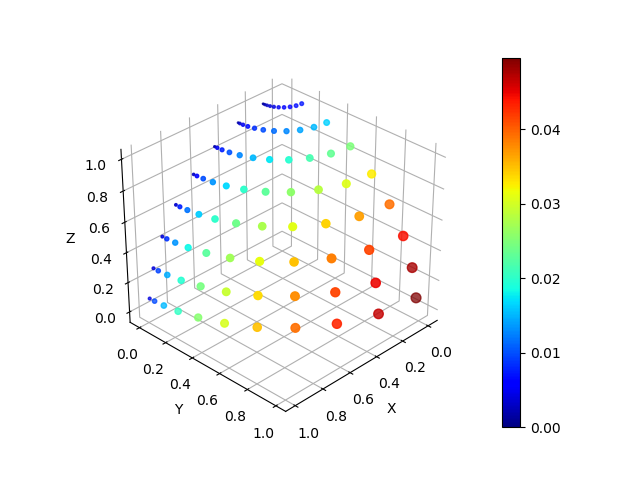
\includegraphics[width=0.7\linewidth]{Figures/Gauss-Legendre-Legendre.png}
\caption{Quadrature points and weights (colors) for the Gauss-Legendre quadrature set for both the polar and azimuthal angles with $N_a=8$ and $N_p=8$.}
\label{fig:s8gausslegendrelegendre}
\end{figure}

\newpage
\subsection{Gauss-Legendre-Chebyshev product quadrature}
Instead of changing the intervals of the integration over the azimuthal angles $\varphi$ we can instead look towards utilizing these intervals by defining
$$
y = cos(\frac{\varphi}{2})
$$
and
$$
\frac{dy}{d\varphi} = -\frac{1}{2}sin(\frac{\varphi}{2}).
$$
Therefore
\beq
d\varphi &= - \frac{2}{sin(\frac{\varphi}{2})}.dy \\
&= - \frac{2}{\sqrt{  1 - cos^2 (\frac{\varphi}{2})    }}.dy\\
\therefore d\varphi &= - \frac{2}{\sqrt{  1 - y^2     }}.dy
\eeq

which can be used in equation \ref{eq:integratevarphi} as

\beq
\int_0^{2\pi} g(\varphi).d\varphi 
&= \int_1^{-1} -2 \frac{g(2cos^{-1}y)}{\sqrt{  1 - y^2     }}.dy \\
&=2 \int_{-1}^{1}  \frac{g(2cos^{-1}y)}{\sqrt{  1 - y^2     }}.dy \\
\eeq

and when we define, for simplicity, $h(y)=g(2cos^{-1}y)$ we get a familiar form

\beqn
\int_0^{2\pi} g(\varphi).d\varphi = 2\int_{-1}^1 \frac{h(y)}{ \sqrt{1-y^2}  }.dy.
\eeqn
\newline
This equation can be approximated with a Gauss-Chebyshev quadrature with abscissae
\beqn
y_j = cos\biggr(  \frac{(2j+1)\pi}{8N_a}  \biggr)
\eeqn

and equal weights
\beqn
w_j = \frac{2\pi}{4N_a}
\eeqn

where $N_a$ is the number of quadrature points per octant, to get the quadrature formula

\beqn
\int_{-1}^1 \frac{h(y)}{ \sqrt{1-y^2}  }.dy \approx \  \sum_{j=0}^{4N_a-1} w_j h(y_j).
\eeqn
\newline
The angles associated with the abscissae are then 
\beqn
\varphi_j = \frac{(2j+1)\pi}{8N_a} 
\eeqn

and we now have a product quadrature of the form

\beqn
\int_0^{2\pi}\int_0^\pi f(\varphi,\theta).sin\theta.d\theta.d\varphi\ 
\approx \  \sum_{j=0}^{4N_a-1} w_j \biggr[
\sum_{i=0} ^{2N_p-1}   w_i f(\varphi_j,\theta_i)
\biggr].
\eeqn
\newline
An example of this quadrature is shown for the first octant in Figure \ref{fig:s8gausslegendrechebyshev} where the colors and dot size indicate the quadrature weight and the dot's position indicates the quadrature point on the unit sphere.
\begin{figure}[h]
\centering
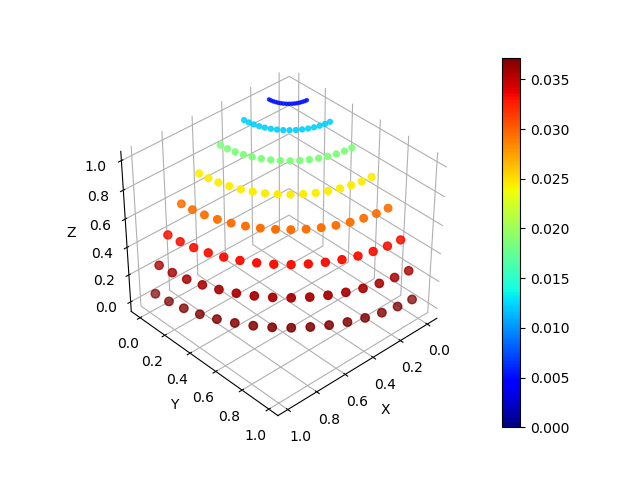
\includegraphics[width=0.7\linewidth]{Figures/Gauss-Legendre-Chebyshev.png}
\caption{Quadrature points and weights (colors) for the Gauss-Legendre quadrature for the polar integration and the Gauss-Chebyshev quadrature for the azimuthal angles with $N_a=8$ and $N_p=8$.}
\label{fig:s8gausslegendrechebyshev}
\end{figure}


\newpage
\subsection{Evaluation of product quadratures}
With the quadrature candidates established we can now look at their performance. The application of the product quadratures is done to calculate the integral
\begin{equation*}
\int_{4\pi} \Psi_g(r,\hat{\Omega}) Y_{\ell m^*}(\hat{\Omega}).d\hat{\Omega} 
\end{equation*}

where the angular flux $\Psi(r,\hat{\Omega})$ is known at the point where the integration is to be performed. Hence we are essentially looking for a function to integrate the spherical harmonic $Y_{lm^*}(\hat{\Omega})$ where, repeated here

$$Y_{\ell m*}(\theta ,\varphi ) = (-1)^mY_{\ell (-m)}(\theta ,\varphi )$$

\begin{equation}
Y_{\ell m} (\theta, \varphi )=
\begin{cases}
(-1)^m \sqrt(2)\sqrt{ \frac{(2\ell + 1)}{4\pi}   \frac{(\ell-|m|)!}{(\ell+|m|)!}}P_{\ell}^{|m|}(cos\theta)sin\ {|m|\varphi}
& \text{if } m < 0 \\
(-1)^m \sqrt(2)\sqrt{ \frac{(2\ell + 1)}{4\pi}   \frac{(\ell-m)!}{(\ell+m)!}}P_{\ell}^{m}(cos\theta)cos\ {m\varphi}
& \text{if } m \ge 0 \\
\end{cases}
\end{equation}
\newline
where the associated Legendre polynomials, $P_\ell^m$ can be determined from

\beqn
P_0^0 &= 1, \quad \quad \quad
P_1^{0} = x, \\
P_\ell^\ell &= - (2\ell-1) \sqrt{1-x^2} \ P_{\ell-1}^{\ell-1}(x) \quad \text{ and}\\
(\ell - m)
P_\ell^m &= (2\ell-1)x \ P_{\ell-1}^m(x) - (\ell+m -1)P_{\ell-2}^m (x).
\eeqn
\newline
An algorithm implementation to evaluate these associated Legendre polynomials is shown below.

\begin{lstlisting}[language=python]
def AssociatedLegendre(ell,m,x):
    if (abs(m)>ell):
        return 0;
    
    #====m=0,l=1
    Pn   = x;
    
    #====m=1,l=1
    Pnpos= -math.sqrt(1-math.pow(x,2));
    #====m=-1,l=1
    Pnneg= -0.5*Pnpos;
    
    #====m=0,l=0
    if (ell==0):
        return 1;
    
    if (ell==1):
        if (m==-1):
            return Pnneg;
        if (m==0):
            return Pn;
        if (m==1):
            return Pnpos;

    Pmlp1 = 0
    if (ell==m):
        Pmlp1 = -(2*ell-1)*math.sqrt(1-math.pow(x,2.0))* \
                AssociatedLegendre(ell-1,ell-1,x)
    else:
        Pmlp1 = (2*ell-1)*x*AssociatedLegendre(ell-1,m,x);
        Pmlp1 = Pmlp1 - (ell+m-1)*AssociatedLegendre(ell-2,m,x)
        Pmlp1 = Pmlp1 / (ell-m)
    
    return Pmlp1 
\end{lstlisting} 

An algorithm implementation of the tesseral spherical harmonics is shown below.

\begin{lstlisting}[language=python]
#============================
def fac(x):
    if (x==0):
        return 1
    if (x==1):
        return 1
    
    return fac(x-1)*x;

#============================
def Min1powerm(m):
    if (m==0):
        return 1;
    if ((m%2)==0):
        return 1
    else:
        return -1

#============================    
def Ylm(ell,m,theta,varphi):
    if (m<0):
        return Min1powerm(m)*math.sqrt( \
               ( (2*ell+1)/(2*math.pi) )* \
               fac(ell-abs(m))/fac(ell+abs(m)) )* \
               AssociatedLegendre(ell,abs(m),math.cos(theta))* \
               math.sin(abs(m)*varphi)
    else:
        return Min1powerm(m)*math.sqrt( \
               ( (2*ell+1)/(2*math.pi) )* \
               fac(ell-m)/fac(ell+m) )* \
               AssociatedLegendre(ell,m,math.cos(theta))* \
               math.cos(m*varphi)
\end{lstlisting} 




\newpage 
\renewcommand{\thefigure}{B\arabic{section}.\arabic{figure}}
\section{More on Spherical Harmonics}
\subsection{Expansion of a function of two angles $f(\varphi,\theta)$}
We seek to expand an angularly dependent function $f(\varphi,\theta)$. Why? Don't know yet, but one such expansion from fundamental theory is spherical harmonics:
\begin{equation} \label{eq:harmonicExpansion}
f(\varphi,\theta) = \sum_{\ell=0}^{\infty}\sum_{m=-\ell}^{\ell}   f_{\ell }^m Y_{\ell }^m(\varphi,\theta  ).
\end{equation}
\newline
This expansion will be very unfamiliar for engineers since most of the scientific computing in common disciplines deal with cartesian coordinates. Unfortunately it will be nearly impossible to explain the development of an expansion of an angular function in spherical harmonics without first exploring the means to calculate its unknowns. To this end let us begin with stating that \textbf{there are two flavors of spherical harmonics}. The regular form $Y_{\ell}^m$, which contains complex numbers (challenging to handle), and a real form $Y_{\ell m}$.
The unknowns in equation \ref{eq:harmonicExpansion} has a trail of components the first of which is
\begin{equation*}
\begin{aligned}
f_{\ell }^m
&=\int _{\hat{\Omega} }f(\varphi,\theta )\,Y_{\ell }^{m^*}(\varphi,\theta)\,d\hat{\Omega} \\
&=\int _{0}^{2\pi }\int _{0}^{\pi } f(\varphi,\theta )Y_{\ell }^{m^*}(\varphi,\theta ) .\sin \theta .d\theta .d\varphi .
\end{aligned}
\end{equation*}

The reader should try to comprehend that the $f_{\ell}^m$ components are almost never computed in this form since doing so means one already has a analytical representation of $f(\varphi,\theta)$. Additionally we have

\begin{equation}
Y_{\ell}^m (\varphi,\theta)= 
(-1)^m \sqrt{
\frac{(2\ell+1)}{4\pi}
\frac{(\ell-m)!}{(\ell+m)!}
}
.P_{\ell}^m (\cos \theta)e^{ (m \varphi)i}
\end{equation}
and its complex conjugate
$$Y_{\ell }^{m^*}(\varphi,\theta) = (-1)^mY_{\ell }^{(-m)}(\varphi,\theta).$$
This form of the spherical harmonics functions can be very unruly and therefore its more common place to calculate them from the real forms as

\begin{equation}
Y_{\ell}^m (\varphi,\theta)=
\begin{cases}
\frac{1}{\sqrt{2}} (Y_{\ell |m|}- i Y_{\ell,-|m|}) & \text{if }m<0 \\
Y_{\ell0} & \text{if } m=0 \\
\frac{(-1)^m}{\sqrt{2}} (Y_{\ell |m|}+ i Y_{\ell,-|m|}) & \text{if }m>0 \\
\end{cases}
\end{equation}
Here the real forms are represented by:
\begin{equation}\label{eq:Ylm}
Y_{\ell m} (\theta, \varphi )=
\begin{cases}
(-1)^m \sqrt(2)\sqrt{ \frac{(2\ell + 1)}{4\pi}   \frac{(\ell-|m|)!}{(\ell+|m|)!}}P_{\ell}^{|m|}(\cos\theta)sin\ {|m|\varphi}
& \text{if } m < 0 \\
\sqrt{ \frac{(2\ell + 1)}{4\pi}} P_{\ell}^{m}(cos\theta) & \text{if } m = 0 \\
(-1)^m \sqrt(2)\sqrt{ \frac{(2\ell + 1)}{4\pi}   \frac{(\ell-m)!}{(\ell+m)!}}P_{\ell}^{m}(\cos\theta)cos\ {m\varphi}
& \text{if } m \ge 0 \\
\end{cases}
\end{equation}
\newline
Finally the associated Legendre polynomials, $P_\ell^m$ can be determined from

\beqn 
P_0^0 &= 1, \quad \quad \quad
P_1^{0} = x, \\
P_\ell^\ell &= - (2\ell-1) \sqrt{1-x^2} \ P_{\ell-1}^{\ell-1}(x) \quad \text{ and}\\
(\ell - m)
P_\ell^m &= (2\ell-1)x \ P_{\ell-1}^m(x) - (\ell+m -1)P_{\ell-2}^m (x).
\eeqn
\newline
With all these unknows we see that before we can calculate the expansion we need to choose the maximum order $L=\ell_{max}$ after which we need to compute each $P_\ell^m$, each $Y_{\ell m}$, each $Y_{\ell}^m$ and each $Y_\ell^{m^*}$. Only then can we compute $f_{\ell}^m$. If we do all the work this way we can approximate some functions.

\subsection{Prototype code for spherical harmonics}
We begin with code to compute the associated Legendre polynomials

\begin{lstlisting}[language=python]
def AssociatedLegendre(ell,m,x):
    if (abs(m)>ell):
        return 0;
    
    #====m=0,l=1
    Pn   = x;
    
    #====m=1,l=1
    Pnpos= -math.sqrt(1-math.pow(x,2));
    #====m=-1,l=1
    Pnneg= -0.5*Pnpos;
    
    #====m=0,l=0
    if (ell==0):
        return 1;
    
    if (ell==1):
        if (m==-1):
            return Pnneg;
        if (m==0):
            return Pn;
        if (m==1):
            return Pnpos;

    Pmlp1 = 0
    if (ell==m):
        Pmlp1 = -(2*ell-1)*math.sqrt(1-math.pow(x,2.0))* \
                AssociatedLegendre(ell-1,ell-1,x)
    else:
        Pmlp1 = (2*ell-1)*x*AssociatedLegendre(ell-1,m,x);
        Pmlp1 = Pmlp1 - (ell+m-1)*AssociatedLegendre(ell-2,m,x)
        Pmlp1 = Pmlp1 / (ell-m)
    
    return Pmlp1 
\end{lstlisting}

\newpage
We then depict code to calculate the real forms of the spherical harmonics

\begin{lstlisting}[language=python]
#============================
def fac(x):
    if (x==0):
        return 1
    if (x==1):
        return 1
    
    return fac(x-1)*x;

#============================
def Min1powerm(m):
    if (m==0):
        return 1;
    if ((m%2)==0):
        return 1
    else:
        return -1

#============================    
def Ylm(ell,m,varphi,theta):
    if (m<0):
        return Min1powerm(m)*math.sqrt( \
               ( (2*ell+1)/(2*math.pi) )* \
               fac(ell-abs(m))/fac(ell+abs(m)) )* \
               AssociatedLegendre(ell,abs(m),math.cos(theta))* \
               math.sin(abs(m)*varphi)
    elif (m==0):
        return math.sqrt( \
               ( (2*ell+1)/(4*math.pi) )* \
               fac(ell-m)/fac(ell+m) )* \
               AssociatedLegendre(ell,m,math.cos(theta))* \
               math.cos(m*varphi)
    else:
        return Min1powerm(m)*math.sqrt( \
               ( (2*ell+1)/(2*math.pi) )* \
               fac(ell-m)/fac(ell+m) )* \
               AssociatedLegendre(ell,m,math.cos(theta))* \
               math.cos(m*varphi)
\end{lstlisting}

And then the complex form of the spherical harmonics
\begin{lstlisting}[language=python]
#============================
def Yl_m(ell,m,varphi,theta):
    v = 0+0j;
    if (m<0):
        v = (1/math.sqrt(2))*complex(Ylm(ell,abs(m),varphi,theta), - \
                                     Ylm(ell,-abs(m),varphi,theta))
    elif (m==0):
        v = complex(Ylm(ell,0,varphi,theta),0)
    else:
        v = Min1powerm(m)* \
        (1/math.sqrt(2))*complex(Ylm(ell,abs(m),varphi,theta), \
                                 Ylm(ell,-abs(m),varphi,theta))
        
    return v
\end{lstlisting}

\newpage
From here we need to have a means to compute the integral

\begin{equation*}
\begin{aligned}
f_{\ell }^m
&=\int _{\hat{\Omega} }f(\varphi,\theta )\,Y_{\ell }^{m^*}(\varphi,\theta)\,d\hat{\Omega} \\
&=\int _{0}^{2\pi }\int _{0}^{\pi } f(\varphi,\theta )Y_{\ell }^{m^*}(\varphi,\theta ) .\sin \theta .d\theta .d\varphi .
\end{aligned}
\end{equation*}

Suppose we have any function of angle \texttt{F0}, \texttt{F1}, \texttt{F2} and so forth we can define a function that will add the complex conjugate of the spherical harmonics with the simple code

\begin{lstlisting}[language=python]
#============================
def Flm(ell,m,varphi,theta):
    return F2(varphi,theta)*Min1powerm(m)* \
           (Legendre.Yl_m(ell,-m,varphi,theta))
\end{lstlisting}

We can then precompute a vector containing all the $f_{\ell m}$ coefficients using either a Riemann integral or a quadrature rule

\begin{lstlisting}[language=python]
GLC = Legendre.Quadrature()
GLC.InitializeWithGLC(8,8)


#=========================== Build flm
L =7
k=-1
flm = np.zeros((L*(L+2)+1),dtype=np.complex_)
for ell in range(0,L+1):
    for m in range(-ell,ell+1):
        k=k+1
        #flm[k] = Legendre.RiemannAngLM(F1lm,ell,m)
        
        #print("l=%f, m=%f, flm=" %(ell,m), end='')
        #print(flm[k])
        flm[k] = Legendre.QuadratureIntegrateLM(Flm,GLC,ell,m)
        print("l=%f, m=%f, flm=" %(ell,m), end='')
        print(flm[k])
\end{lstlisting}

Finally we can compute a representation of the expansion over the span of $\varphi$ using the code

\begin{lstlisting}[language=python]
#============================ Build yi1
Ni1=200
varphi1=np.linspace(0,2*math.pi,Ni1)
yi1=np.zeros((Ni1))

for i in range(0,Ni1):
    yi1[i]= 0;
    v = 0+0j
    k=-1;
    for ell in range(0,L+1):
        for m in range(-ell,ell+1):
            k=k+1
            v=v+(flm[k])* \
            (Legendre.Yl_m(ell,m,varphi1[i],math.pi/2))
            yi1[i] = v.real
\end{lstlisting}

\subsubsection{Approximating an isotropic flux}
The simplest function to represent is an isotropic flux (i.e. $f(\varphi,\theta)=1$). Such a function is perfectly capture with $L=0$, i.e. a single expansion, as shown in Figure \ref{fig:ylmf0}. This is not surprising since the combination of spherical harmonics with order and moment zero results in $\sqrt{\frac{1}{4\pi}} \stimes \sqrt{\frac{1}{4\pi}}$ which integrates to unity and hence the original function is recovered.
\begin{lstlisting}[language=python]
def F0(varphi,theta):
    return 1
\end{lstlisting}
\begin{figure}[H]
\centering
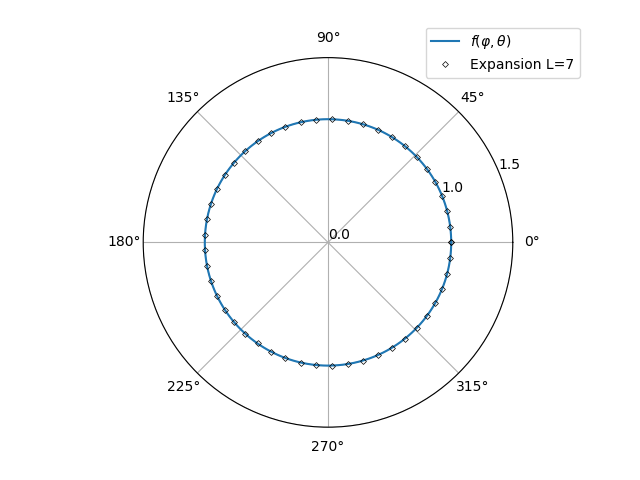
\includegraphics[width=0.8\linewidth]{Figures/Ylm_f0}
\caption{Approximation of a pure isotropic function with spherical harmonics. The plot is shown for the azimuthal angle $\varphi$ only.}
\label{fig:ylmf0}
\end{figure}

\subsubsection{Approximating an anisotropic but smooth flux}
We can construct an anisotropic function of azimuthal angle as
$$
f(\varphi,\theta) = 1+\cos (4\varphi)
$$

\begin{lstlisting}[language=python]
def F1(varphi,theta):
    return 1.0+0.1*math.cos(varphi*4)
\end{lstlisting}

Such a function requires a few more orders of spherical harmonics in order to capture the shape and, as shown in Figure \ref{fig:ylmf7}, $L=7$ closely resembles the shape. A function of this shape could appear in a fuel assembly lattice where the effective scattering and absorbtion is a strong function of azimuthal angle.

\begin{figure}[H]
\centering
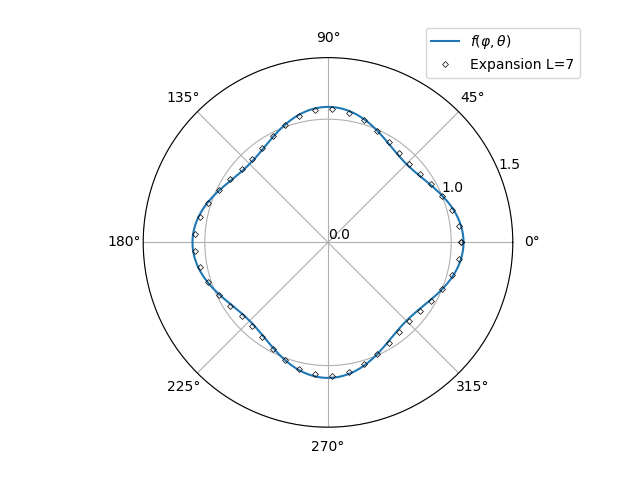
\includegraphics[width=0.8\linewidth]{Figures/Ylm_f7}
\caption{Approximation of an anisotropic smooth function with spherical harmonics. The plot is shown for the azimuthal angle $\varphi$ only. The radial dimension represents the flux magnitude.}
\label{fig:ylmf7}
\end{figure}

\newpage
\subsubsection{Approximating a directional flux (i.e. anisotropic + not-smooth)}
As a final consideration we try to construct a function that is very angular, like a beam. Such a function of angle could be
\begin{equation*}
f(\varphi,\theta) = 
\begin{cases}
\frac{2}{10} & \text{if } \quad \varphi<\frac{7}{8}\pi \\
\frac{2}{10} + \frac{6}{5}\cos (4\varphi) & \text{if }\quad \frac{7}{8}\pi \le \varphi \le \frac{9}{8}\pi\\
\frac{2}{10} & \text{if }\quad \ \varphi>\frac{9}{8}\pi \\
\end{cases}
\end{equation*}

\begin{lstlisting}[language=python]
def F2(varphi,theta):
    if (varphi<(7*math.pi/8)):
        return 0.2;
    if (varphi>(9*math.pi/8)):
        return 0.2;
    
    return 1.2*math.cos(varphi*4)+0.2
\end{lstlisting}

As expected a total number of 12 spherical harmonic orders are required to accurately represent such a directional flux (see Figure \ref{fig:ylmf12}). An additional 2D plot is shown in Figure \ref{fig:ylmf12b} which more clearly shows the oscillations of the expansion at the directions not aligned with the directional nature of the function.

\begin{figure}[H]
\centering
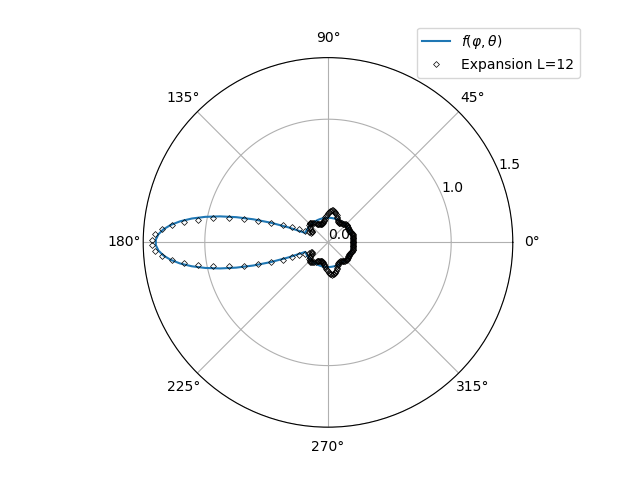
\includegraphics[width=0.8\linewidth]{Figures/Ylm_f12}
\caption{Approximation of an anisotropic smooth function with spherical harmonics. The plot is shown for the azimuthal angle $\varphi$ only. The radial dimension represents the flux magnitude.}
\label{fig:ylmf12}
\end{figure}

\begin{figure}[H]
\centering
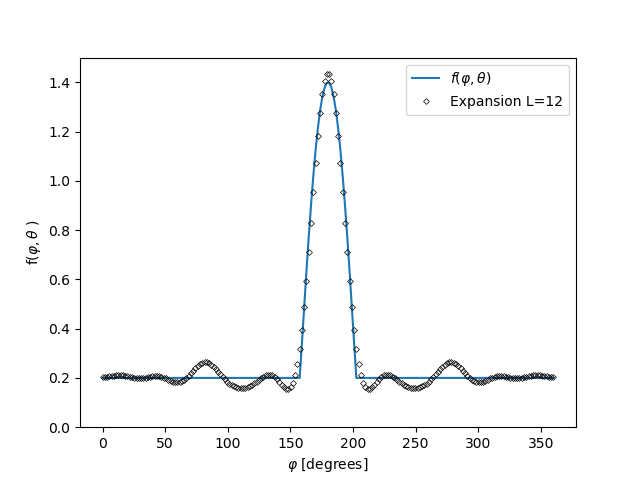
\includegraphics[width=0.8\linewidth]{Figures/Ylm_f12b}
\caption{Approximation of an anisotropic smooth function with spherical harmonics. The plot is shown for the azimuthal angle $\varphi$ only. }
\label{fig:ylmf12b}
\end{figure}

\subsection{Prototype code for real form of the spherical harmonics}
For the real form of the spherical harmonics we have a slightly modified real form 

\beqn
Y_{\ell m} (\theta, \varphi )=
\begin{cases}
 \sqrt(2)\sqrt{ \frac{(2\ell + 1)}{4\pi}   \frac{(\ell-|m|)!}{(\ell+|m|)!}}P_{\ell}^{|m|}(\cos\theta)sin\ {|m|\varphi}
& \text{if } m < 0 \\
\sqrt{ \frac{(2\ell + 1)}{4\pi}} P_{\ell}^{m}(cos\theta) & \text{if } m = 0 \\
 \sqrt(2)\sqrt{ \frac{(2\ell + 1)}{4\pi}   \frac{(\ell-m)!}{(\ell+m)!}}P_{\ell}^{m}(\cos\theta)cos\ {m\varphi}
& \text{if } m \ge 0 \\
\end{cases}
\eeqn

and the expansion coefficients are also different

\beqn 
f(\varphi,\theta) = \sum_{\ell = 0}^\infty \sum_{m=-\ell}^{\ell} f_{\ell m} Y_{\ell m}(\varphi,\theta)
\eeqn 

where
$$
f_{\ell m} = \int_{0}^{2\pi} \int_0^\pi f(\varphi,\theta)Y_{\ell m}(\varphi,\theta).sin\theta.d\theta.d\varphi
$$

for which the code is

\begin{lstlisting}[language=python]
#============================    
def Ylmcoeff(ell,m,varphi,theta):
    if (m<0):
        return math.sqrt( \
               ( (2*ell+1)/(2*math.pi) )* \
               fac(ell-abs(m))/fac(ell+abs(m)) )* \
               AssociatedLegendre(ell,abs(m),math.cos(theta))* \
               math.sin(abs(m)*varphi)
    elif (m==0):
        return math.sqrt( \
               ( (2*ell+1)/(4*math.pi) )* \
               fac(ell-m)/fac(ell+m) )* \
               AssociatedLegendre(ell,m,math.cos(theta))* \
               math.cos(m*varphi)
    else:
        return math.sqrt( \
               ( (2*ell+1)/(2*math.pi) )* \
               fac(ell-m)/fac(ell+m) )* \
               AssociatedLegendre(ell,m,math.cos(theta))* \
               math.cos(m*varphi)
\end{lstlisting}

And

\begin{lstlisting}[language=python]
def Flm(ell,m,varphi,theta):
    return F3(varphi,theta)* \
           (Legendre.Ylmcoeff(ell,m,varphi,theta))
           
#=========================== Build flm
L =12
k=-1
flm = np.zeros((L*(L+2)+1),dtype=np.complex_)
for ell in range(0,L+1):
    for m in range(-ell,ell+1):
        k=k+1
        #flm[k] = Legendre.RiemannAngLM(F1lm,ell,m)
        
        #print("l=%f, m=%f, flm=" %(ell,m), end='')
        #print(flm[k])
        flm[k] = Legendre.QuadratureIntegrateLM(Flm,GLC,ell,m)
        print("l=%f, m=%f, flm=" %(ell,m), end='')
        print(flm[k])

#============================ Build yi1
Ni1=400
varphi1=np.linspace(0,2*math.pi,Ni1)
yi1=np.zeros((Ni1))

for i in range(0,Ni1):
    yi1[i]= 0;
    v = 0
    k=-1;
    for ell in range(0,L+1):
        for m in range(-ell,ell+1):
            k=k+1
            v=v+(flm[k])* \
            (Legendre.Ylmcoeff(ell,m,varphi1[i],math.pi/2))
            yi1[i] = v
\end{lstlisting}



\newpage 
\renewcommand{\thefigure}{C.\arabic{figure}}
\section{Creating simple materials for testing}
Neutral particle transport involves three basic processes:
\begin{itemize}
\item Absorption. The elimination of the particle from a current group
\item Scattering. Change in angle and group essentially removing the particle from the group-angle pair.
\item Source. Both in the form of a fixed source and as reactions to absorption processes (i.e. (n,n), (n,2n), (n,fission), etc.)
\end{itemize}

We also have a fundamental definition that the total removal process is the sum of the absorption process and the scattering process. In terms of nuclide cross-sections we can write this as

$$
\sigma_t = \sigma_a + \sigma_s 
$$
Where $\sigma_t$, $\sigma_a$ and $\sigma_s$ represent the total-, absorption- and scattering cross-sections respectively.

\chead{Scattering kinematics}
\subsection{Simple particle-nuclide scattering processes}

\begin{figure}[H]
\centering
\includegraphics[width=0.85\linewidth]{LatexDraw/CollisionKinematics1}
\caption{Collision kinematics of a stationary nuclide in both the laboratory reference frame and the center-of-mass reference frame.}
\label{fig:collisionkinematics1}
\end{figure}


Let us consider a statyionary target nucleus $X_Z^A$ suspended in space and a particle moving towards this nucleus (from left to right) at velocity $\text{v}_{L}$, where $L$ denotes the laboratory reference frame (i.e. the one we are living in) as denoted in Figure \ref{fig:collisionkinematics1}. Assuming the target nucleas is at rest (an invalid assumption that will be treated later) with velocity $V_L$ we know the energies associated with these particles to be 
\beq
E_L &= \frac{1}{2} m \text{v}_L^2 \\
E_{L_A} &= \frac{1}{2} M \cancelto{0}{V_L^2}
\eeq
where $E_L$ is the energy of the particle and $E_{L_A}$ is the energy of the target nucleus, both in the laboratory reference frame, and $m=1$ is the mass of the particle and $M=A$ is the mass of the target nucleus. Fortunately the derivation of the mass-momentum equations relating the center-of-mass energies and angles to the laboratory reference frame quantities are comprehensively depicted in the textbook by Duderstadt and Hamilton \cite{Duderstadt}. In this book the scattering angle in the laboratory reference frame, $\theta_L$, is related to the scattering angle in the center-of-mass reference frame, $\theta_c$, as

\beqn \label{eq:thetaLvsthetac}
\tan \theta_L = \frac{  \sin \theta_c    } {  \frac{1}{A} +\cos \theta_c     }.
\eeqn 
Associated with this, \cite{Duderstadt} also derives the particle energy change $E_L \to E_L'$ as 

\beqn 
E_L' = \biggr[
\frac{  (1+\alpha) + (1-\alpha)\cos \theta_c   }{2}
\biggr] E_L
\eeqn 

where $\alpha = ( \frac{A-1}{A+1})^2$. For light nuclei, where one can assume the scattering angle in the center-of-mass frame is isotropic \cite{Duderstadt} we can determine the probability distribution function for scattering through an angle $\theta_L$. From equation \ref{eq:thetaLvsthetac} we can get $\theta_L$ as 

\beqn \label{eq:thetaLvsthetac2} 
\theta_L = 
\begin{cases}
\pi + 
\cos^{-1} \biggr(
\frac{\sin \theta_c}{ \frac{1}{A} + \cos \theta_c      }
\biggr)
& \text{if } (\frac{1}{A} + \cos \theta_c) < 0 \\
\frac{\pi}{2} & \text{if } (\frac{1}{A} + \cos \theta_c) = 0 \\
\cos^{-1} \biggr(
\frac{\sin \theta_c}{ \frac{1}{A} + \cos \theta_c      }
\biggr)
& \text{if } (\frac{1}{A} + \cos \theta_c) > 0 \\
\end{cases}
\eeqn 
\newline
Since $\cos \theta_c$, $\theta_c \in [0,\pi]$, is essentially our cumulative probability when linearly mapped to $[0,1]$ we require the inverse of equation \ref{eq:thetaLvsthetac}. Therefore we begin by setting $x=\cos \theta_c$ and inserting it into equation \ref{eq:thetaLvsthetac2}

\beq 
\tan \theta_L = \frac{ \sqrt{1-x^2}      }{ \frac{1}{A} + x}
\eeq 

 and for simplicity we set the unknowns to constants
 \beq 
C &= \frac{ \sqrt{1-x^2}      }{ B + x} \\
C(B+x) &= \sqrt{1-x^2}  \\
C^2(x^2+2Bx + B^2) &= 1-x^2 \\
C^2x^2+2BC^2x + B^2C^2 &= 1 -x^2 \\
(C^2+1) x^2 +2BC^2 x + B^2C^2 -1 &= 0
 \eeq 
  which is now in the familiar form $ax^2 + bx +c =0$ for which we complete the square to find
  
 \beq
 x &= \frac{  -2BC^2   \pm \sqrt{  4B^2C^4 - 4(C^2+1)(B^2C^2-1)    }     }{2(C^2+1)}\\
 \therefore x&= \frac{  -2BC^2   \pm 2C\sqrt{  1-B^2+\frac{1}{C^2}   }     }{2(C^2+1)}.
 \eeq
The two possible $x$ values obtained this way was incurred because we applied a square to remove the square-root term and therefore will give us the angle corresponding to $\tan \theta_L$ as well as $-\tan \theta_L$. Since we know that we started with a positive $\tan \theta_L$ we are only interested in the solution

 \beqn
 \cos \theta_c =  x = f(\theta_L)=g(\mu) &= \frac{  -2BC^2  + 2C\sqrt{  1-B^2+\frac{1}{C^2}   }     }{2(C^2+1)} .
 \eeqn
 
 And therefore our mapping to a cumulative probability distribution becomes
 
 \beqn 
\int_{-1}^1 P(\mu).d\mu = \frac{g(\mu)-1}{2} 
 \eeqn 
 where $B{=}1/A$ and $C{=} \tan ( \cos^{-1} \mu)$. The cumulative probability function for different masses of the target nucleus is shown in Figure \ref{fig:scatanglevsa}. Obtaining the probability density function, $P(\mu)$ is then a simple differentiation that can be done numerically 
 
\beqn
P(\mu)=\frac{1}{2} \frac{dg}{d\mu}
\eeqn  
for which the results are shown in Figure \ref{fig:scatproblevsa}. The algorithm applied to find $P(\mu)$ is shown below

\begin{lstlisting}[language=python]
#============================
def ThetaC(thetaL,A):
    B = 1/A
    if (thetaL == (math.pi/2)):
        C=1
    else:
        C = min(math.tan(thetaL),1.0e6)
    
    root = (1-B**2+1/(C**2))
    
    x1 = (-2*B*C**2 + 2*C*math.sqrt(root))/2/(C**2+1)
    #x2 = (-2*B*C**2 - 2*C*math.sqrt(root))/2/(C**2+1)
    
    #Safety catches
    if (x1>1.0):
        return math.acos(1)
    if (x1<-1.0):
        return math.acos(-1)
    
    return math.acos(x1)
\end{lstlisting}

\newpage
\begin{lstlisting}[language=python]
#============================ Probability scattering mu
def Pmu(mu,A):
    thetaLA = math.acos(mu-0.0000001)
    thetaLB = math.acos(mu+0.0000001)
    thetacA = ThetaC(thetaLA,A)
    thetacB = ThetaC(thetaLB,A)
    CPLA    = 0.5-0.5*math.cos(thetacA)
    CPLB    = 0.5-0.5*math.cos(thetacB)
    return -(CPLB - CPLA)/0.0000002
\end{lstlisting}



\begin{figure}[H]
\centering
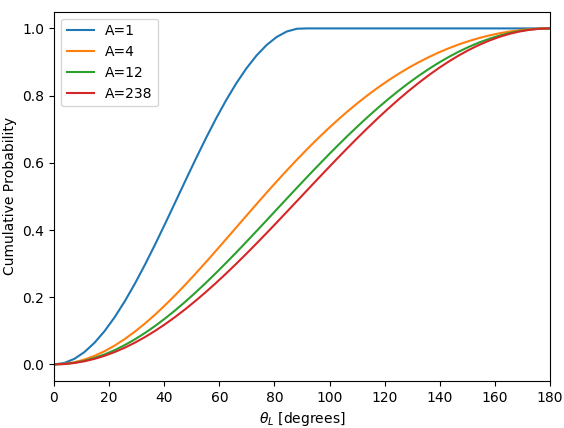
\includegraphics[width=0.7\linewidth]{Figures/ScatAnglevsA}
\caption{Cumulative probability distribution for a particle scattering off a stationary nucleus of mass A.}
\label{fig:scatanglevsa}
\end{figure}

\begin{figure}[H]
\centering
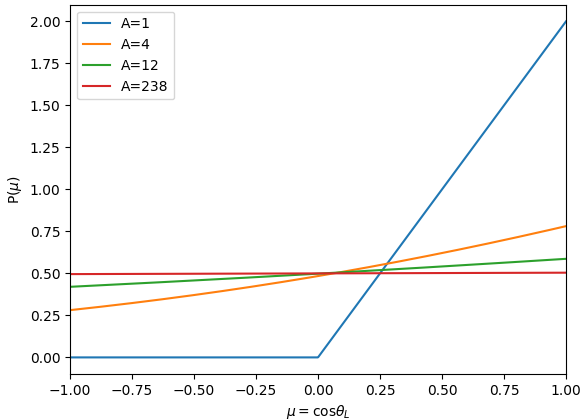
\includegraphics[width=0.7\linewidth]{Figures/ScatProbvsA}
\caption{Probability distribution for a particle scattering off a stationary nucleus of mass A.}
\label{fig:scatproblevsa}
\end{figure}



\subsection{Combining probabilities}
Now, since $\mu$ corresponds to a discrete $\theta_c$ which also corresponds to a discrete $\frac{E_L'}{E_L}$, the kernel value $K(\mu,E'\to E)$ also will have only discrete points where it is non-zero, i.e.

\beq
K(\mu,E' \to E)=
\begin{cases}
P(\mu)P(E'\to E)    &, \text{if } E' - \biggr[
\frac{  (1+\alpha) + (1-\alpha) g(\mu)   }{2}
\biggr] E = 0 \\
0 &, otherwise
\end{cases}
\eeq 

This discrete behavior requires significant numerical effort to resolve, however, multi-group integrations of the source- and destination energy groups alleviates this somewhat since

\beq 
K(\mu,E_{g'} \to E_g) &=
\int_{E_{g+1}'}^{E_g'} \int_{E_{g+1}}^{E_g} K(\mu,E' \to E).dE.dE' \\
&=P(\mu)P(E_{g'}\to E_g) 
\eeq 
\newline
An algorithm to implement this kernel is shown below
\newpage
\begin{lstlisting}[language=python]
def Kernel(mu,gprime,g,Eg,A,Ng=1000):
    #=== Bin boundaries
    Eiupp = Eg[gprime]
    Eilow = Eg[gprime+1]
    Efupp = Eg[g]
    Eflow = Eg[g+1]
    
    dEi = (Eiupp - Eilow)/Ng
    binWidth = (Efupp-Eflow)
    
    sumprobs=0
    thetaL = math.acos(mu)
    thetac = ThetaC(thetaL,A)
    muc = math.cos(thetac)
    for iE in range(0,Ng):
        Ein = Eilow + dEi/2 + dEi*iE        
        Eout=Ef(muc,A,Ein)
        
        if ((Eout<=Efupp) and (Eout>=Eflow)):
            sumprobs = sumprobs + 1/Ng
    
    return sumprobs*Pmu(mu,A)
\end{lstlisting}

In order to test the multi-group implementation of this kernel we can build a simple 10 group energy discretization $E\in [0,1]$ MeV with linearly spaced bins

\begin{lstlisting}[language=python]
G = 10
Eg = np.linspace(1,0,G+1)
\end{lstlisting}

The requirement here is that the continuous form obeys

\beq 
\int_{-1}^1 \int_0^\infty K(\mu,E' \to E).dE.d\mu = 1
\eeq 

and therefore the multi-group form must obey
\beq 
\int_{-1}^1 \biggr( \sum_{g=0}^G  K(\mu,E_{g'} \to E_g) \biggr).d\mu = 1.
\eeq 
 The code to implement this integration is
 
\begin{lstlisting}[language=python]
Np=100
mu=np.linspace(-0.9999,0.9999,Np)
ydis=np.zeros((Np))
sumofdis=0
sumovergroupsdis=0
for i in range(0,Np):
    for gdes in range(0,G):
        sumovergroupsdis=sumovergroupsdis+ \
                         Kernel(mu[i],gprime,gdes,Eg,A)*(2/Np)
\end{lstlisting}

and proves that the integral is unity as intended. Another test is to integrate over all angle with

\beq 
&\int_{4\pi} \biggr( \sum_{g=0}^G  K(\Omega' \bigcdot \Omega,E_{g'} \to E_g) \biggr).d\Omega' \\
=&\int_{0}^{2\pi} \int_0^\pi  
\biggr( \sum_{g=0}^G  K(\Omega' \bigcdot \Omega,E_{g'} \to E_g) \biggr)
.\sin \theta' .d\theta'.d\varphi' \\
=&2\pi
\eeq 

where $\Omega' = [\sin\theta' . \cos \varphi', \sin\theta' . \sin \varphi', \cos \theta']$ and $\Omega$ is chosen arbitrarily (i.e. $\Omega=[1,0,0]$). The code to compute this integral, using the previous denoted 10-group energy structure, as well as scattering from group 0, is shown below

\begin{lstlisting}[language=python]
Np = 100
Na = 200
polar = np.linspace(0.0001,math.pi*0.9999,Np)
azimu = np.linspace(0.0001,2*math.pi*0.99999,Na)
dtheta = (math.pi)/Np
dvarphi= (math.pi*2)/Na

nref = np.array([1.0,0.0,0.0])
ndir = np.array([0.0,0.0,0.0])

sumprob=0.0
gprime=0
for i in range(0,Na):
    print(i)
    for j in range(0,Np):
        varphi = azimu[i]
        theta  = polar[j]
        
        ndir[0] = math.sin(theta)*math.cos(varphi)
        ndir[1] = math.sin(theta)*math.sin(varphi)
        ndir[2] = math.cos(theta)
        
        mu = np.dot(ndir,nref)
        
        for gdes in range(0,G):
            sumprob=sumprob+ \
              Kernel(mu,gprime,gdes,Eg,A)*math.sin(theta)*dtheta*dvarphi
\end{lstlisting}

Indeed this does then integrate to $2\pi$.

\newpage
\subsection{Legendre expansion of the scattering term}
The discrete ordinates method involves the expansion of the scattering term using Legendre polynomials as basis functions. This expansion is of the form

\begin{align*}
K(\mu,E_{g'} {\to} E_g) &= \sum_{\ell=0}^\infty \frac{2\ell+1}{2} P_\ell (\mu) K_\ell (E_{g'} {\to }E_g)
\end{align*}
where the expansion coefficients are given by
\begin{align*}
K_\ell(E_{g'} {\to} E_g) &= \int_{-1}^1 K(\mu,E_{g'} {\to} E_g).P_\ell (\mu).d\mu
\end{align*}

The code to compute the expansion coefficients requires just a small modification of the multi-group kernel in the sense that the Kernel is multiplied by the Legendre polynomial. The code is shown below

\begin{lstlisting}[language=python]
def KernelL(ell,gprime,g,Eg,A):
    groupprob=0
    Np=800
    mu=np.linspace(-0.9999,0.9999,Np)
    dmu = (0.9999*2)/Np
    print("Integrating group %d to %d moment %d" %(gprime,g,ell))
    for i in range(0,Np):
        groupprob = groupprob + Kernel(mu[i],gprime,g,Eg,A)* \
             Legendre.Legendre(ell,mu[i])*dmu
    
    return groupprob
\end{lstlisting}

We can now decide to truncate our expansion at the $L$-th moment and precompute the expansion coefficient $K_\ell(E_{g'} {\to} E_g)$ with an example scattering from group $g'=0$ to group $g=1$ the code is

\begin{lstlisting}[language=python]
L=10
KL=np.zeros((L+1))
gprime = 0
g=1
sumgroups=0
for ell in range(0,L+1):
    KL[ell] = KernelL(ell,gprime,g,Eg,A)
\end{lstlisting}

We can now compute the discrete and expanded form as a function of $\mu$ for which the code is shown below. A graphical plot of the expanded and discrete form is shown, for different orders of expansion, in Figure  \ref{fig:kernelg0tog1}.
\newpage
\begin{lstlisting}[language=python]
#============================ Discrete form vs Expansion for Group 0 to 1        
Np=100
mu=np.linspace(-0.9999,0.9999,Np)
yexp=np.zeros((Np))
ydis=np.zeros((Np))
sumofdis=0
sumofexp=0
sumovergroupsdis=0
for i in range(0,Np):
    yexp[i] = expansion(L,mu[i],KL)
    ydis[i] = Kernel(mu[i],gprime,g,Eg,A)
    sumofexp=sumofexp+yexp[i]*(2/Np)
    sumofdis=sumofdis+ydis[i]*(2/Np)
    
    for gdes in range(0,G):
        sumovergroupsdis=sumovergroupsdis+ \
                         Kernel(mu[i],gprime,gdes,Eg,A)*(2/Np)
\end{lstlisting}

\begin{figure}[H]
\centering
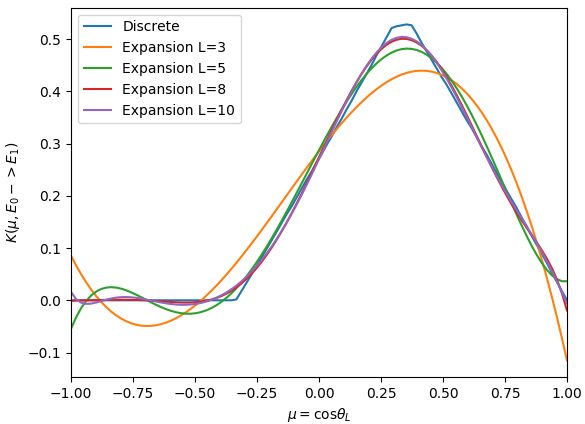
\includegraphics[width=0.7\linewidth]{Figures/KernelG0toG1}
\caption{Kernel function for a particle scattering off of a stationary carbon nuclear ($A=12$) and scattering from group 0 to 1.}
\label{fig:kernelg0tog1}
\end{figure}




\newpage
\renewcommand{\thefigure}{D\arabic{section}.\arabic{figure}}
\chead{Quadrature rules for integration of triangle space}
\section{Quadrature rule for integration of triangle space} \label{appendix:trianglequadrature}
We seek an integral of a function in triangle space $T_{sp}$ in the form

\beq 
\int \int_{T_{sp}} f(x,y).dx.dy = \sum_{i=0}^{N-1} w_i f(x_i,y_i).
\eeq 

Furthermore we know that in the finite element method with only linear shape functions we will at most have polynomials of degree 2 therefore we can devise a set of test functions

\beq 
&f(x,y) = 1    &&\int_{0}^1 \int_0^{1-y} 1.dx.dy = \frac{1}{2} = \sum_{i=0}^{N-1} w_i\\
&f(x,y) = x    &&\int_{0}^1 \int_0^{1-y} x.dx.dy = \frac{1}{6} = \sum_{i=0}^{N-1} w_i x_i\\
&f(x,y) = y    &&\int_{0}^1 \int_0^{1-y} y.dx.dy = \frac{1}{6} = \sum_{i=0}^{N-1} w_i y_i\\
&f(x,y) = xy  & &\int_{0}^1 \int_0^{1-y} xy.dx.dy = \frac{1}{24} = \sum_{i=0}^{N-1} w_i x_i y_i\\
&f(x,y) = x^2    &&\int_{0}^1 \int_0^{1-y} x^2.dx.dy = \frac{1}{12} = \sum_{i=0}^{N-1} w_i x_i^2\\
&f(x,y) = y^2    &&\int_{0}^1 \int_0^{1-y} y^2.dx.dy = \frac{1}{12} = \sum_{i=0}^{N-1} w_i y_i^2\\
\eeq 

With $N=3$ a symmetric solution is obtained with

\beq
w_i &= \frac{1}{6} \\
x_0,y_0 &= ( \frac{1}{6}, \frac{1}{6}) \\
x_1,y_1 &= ( \frac{4}{6}, \frac{1}{6}) \\
x_2,y_2 &= ( \frac{1}{6}, \frac{4}{6}) \\
\eeq 
which is not a unique solution.


\newpage
\renewcommand{\thefigure}{D\arabic{section}.\arabic{figure}}
\chead{Quadrature rules for integration of tetrahedron space}
\section{Quadrature rule for integration of tetrahedron space} \label{appendix:tetrahedronquadrature}
The study of quadratures for tetrahedrons is a deeply mathematical topic one that is outside the scope of this study. As with the two dimensional case, and since we will limit our study to piece-wise linear shape functions we will limit our quadrature set to a minimum degree of precision of 2. Meaning we only need to exactly integrate polynomials of to the second degree. For tetrahedons, in natural coordinates, quadrature sets are available in \cite{quadraturerulestet}. For this study the weights and quadrature points as shown in Table below will be used.

\begin{table}[H] \label{tbl:qpointstet}
\centering
\begin{tabular}{|l|l|l|l|l|}
\hline
\textbf{Point} & \textbf{weights} & \textbf{X}  & \textbf{Y}  & \textbf{Z}  \\ \hline
0              & 0.25             & 0.585410197 & 0.138196601 & 0.138196601 \\ \hline
1              & 0.25             & 0.138196601 & 0.138196601 & 0.138196601 \\ \hline
2              & 0.25             & 0.138196601 & 0.138196601 & 0.585410197 \\ \hline
3              & 0.25             & 0.138196601 & 0.585410197 & 0.138196601 \\ \hline
\end{tabular}
\caption{Quadrature points and weights used for tetrahedron elements.}
\end{table}

\end{appendices}

\newpage
\chead{References}
\begin{thebibliography}{1}
    
    \bibitem{roots} Barrera-Figueroa V., et al. {\em Multiple root finder algorithm for Legendre and Chebyshev polynomials via Newton’s method}, Annales Mathematicae et Informaticae, volume 33, pages 3-13, 2006
    
    \bibitem{Lewis} Lewis E.E, Miller W.F. {\em Computational Methods of Neutron Transport}, John Wiley \& Sons, 1984, ISBN 0-471-09245-2
    
    \bibitem{Duderstadt} Duderstadt J.J., Hamilton L.J., {\em Nuclear Reactor Analysis}, John Wiley \& Sons, 1976.
    
     \bibitem{BaileyAdamsPWLPolygons}  Bailey T.S., Chang J.H., Adams M.L., {\em A Piecewise Linear Discontinous Finite Element spatial discretization of the transport equation in 2D Cylindrical Geometry}, 2009 International Conference on Advances in Mathematics, Computational Methods, and Reactor Physics, 2008.
    
    \bibitem{BaileyAdamsPWBLPolygons}  Bailey T.S., Warsa J.S., Chang J.H., Adams M.L., {\em A Piecewise Bi-linear Discontinous Finite Element spatial discretization of the S$_n$ transport equation}, International Conference on Mathematics and Computational Methods Applied to Nuclear Science and Engineering, 2011.
    
    \bibitem{MathisFunMatrixInverse} Pierce, Rod. {\em Inverse of a Matrix using Minors, Cofactors and Adjugate} Math Is Fun. Ed. Rod Pierce. 22 Nov 2018. 1 Jan 2019 http://www.mathsisfun.com/algebra/matrix-inverse-minors-cofactors-adjugate.html
    
    \bibitem{quadraturerulestet} Engels H., Zienkiewicz O., {\em Quadrature Rules for Tetrahedrons}, http://people.sc.fsu.edu/~jburkardt/datasets/quadrature\_rules\_tet/quadrature\_rules\_tet.html, accessed January 1, 2019.
    
    \bibitem{BaileyAdamsPolyhedral} Bailey T.S., Adams M.L., Yang B., Zika M.R., {\em A piecewise linear finite element discretization of the diffusion equation for arbitrary polyhedral grids}, Journal of Computational Physics 227 (2008) 3738–3757, 2007
    
    \bibitem{delaunay} Cheng et al, {\em Delaunay Mesh Generation}, Chapman \& Hall/CRC Computer \& Information Science Series, 2013
    
    \bibitem{AdamsSPDS} Adams M.P., Hawkins W.D., Adams M.L., {\em Managing Information Flow in Graph Traversals}, Texas A\&M University, November 2018
    
    \bibitem{ProvablyOptimalSweep} Adams et. al, ``PROVABLY OPTIMAL PARALLEL TRANSPORT SWEEPS ON
    SEMI-STRUCTURED GRIDS", archived article for submission, June 2019.
    
    
\end{thebibliography}





\end{document}